% Mingyu Xia (夏明宇, Westlake ID: 20251202247) Homework #i
\documentclass[11pt]{whatsnote}

\coverset{
  title   = Advanced Statistics Mechanics,
  author  = \ttfamily \textsc{Mingyu Xia},
  afill   = PhD @Westlake University,
  date    = November 2025,
  extinfo = {\includegraphics[width = .1\paperwidth]{myhsia_seal}},
  head    = universe.pdf,
  clogo   = cat.pdf,
  llogos  = {mouse1.png, mouse2.png,
             mouse4.png, mouse5.png}
}
\usepackage{pdfpages, esint}
\usepackage[fontset = fandol, scheme = plain]{ctex}

\begin{document}

\maketitle[yellow!50!violet]
\frontmatter
\tableofcontents
\mainmatter

\chapter{Review: Basic Concepts of Thermodynamics}

\section{Definitions}

\begin{definition}[Equilibrium State]
  在没有外界影响的条件下,物体部分的长时间不发生变化的状态.
\end{definition}
\begin{definition}[热平衡定律]
  A 与 B 平衡,B 与 C 平衡,则 A 与 C 平衡.
\end{definition}
\begin{definition}[Temperature]
  衡量物体间是否热平衡的物理量称为温度,一切互为热平衡的物体温度相等.
\end{definition}
\begin{definition}[温标]
  确定温度具体数值的规则叫温标
\end{definition}
\begin{definition}[物态方程]
  \begin{description}
    \item[几何变量] $V$, $A$, $L$
    \item[力学变量] $p$, $\sigma$, $F$
    \item[电磁变量] $\bm E$, $\bm p$, $\bm H$, $\bm M$
    \item[化学变量] $\mu$
  \end{description}
\end{definition}
\begin{equation}
  T = f(p, V, ...)
\end{equation}
\begin{definition}[内能]
  绝热过程(没有热量/能量交换的过程)中外界对物体做功只与初态和末态有关,
  初态和终态的内能差 $U_2 - U1 = W_a \qq{外界对物体的绝热功}$
\end{definition}

\begin{definition}[热力学第一定律]
  推广到非绝热过程,系统从外界吸热,$Q = U_2 - U_1 - W_0$(能量守恒).
\end{definition}

\begin{definition}[热容]
  \begin{equation}
    C_y = \odv{Q_y}T, \qq{$y$ 是一个不变的量}
  \end{equation}
  如果 $y = V$,称为定容;$y = p$,称为定压.

  比热 $C/V$
\end{definition}

\begin{definition}
  内能是态函数,$H = U + pV$,称为焓
  
  绝热过程中,$\Delta H = W_a$.

  等压过程中,$p$ 固定 $\Delta H = Q_p$.

  Entropy: 对可逆过程,态函数
  \begin{equation}
    \Delta S = S - S_0 = \int_\text{Initial State}^\text{Final State} \frac{\d Q}{T}
  \end{equation}
\end{definition}

\begin{definition}[热力学第二定律]
  \begin{equation}
    \Delta S \geq \int_{(i)}^{(f)} \frac{\d Q}T
  \end{equation}
\end{definition}

\begin{definition}[热力学基本方程]
  \begin{equation}
    \d U = T\d S = \sum_i F_n \d y_i
    p-V-T: \d U = T\d S - p\d V
  \end{equation}
  自由能:$F =  U - TS$
  $\d F = \d Y - \d(TS)$, 
  $\d F = -S\d T - p\d N$
\end{definition}

\begin{definition}[G.bbs 自由能: $G = F + pV$]
  \begin{equation}
    \d G = -S\d T + V\d p
  \end{equation}
  means 等温等压过程中,$G$ 又不增加.
\end{definition}

\section{均匀系(单相系)的平衡}

均匀系 $p-V-T$:
\begin{equation}
  \d U = T\d S - p\d V ~ (S,V)
\end{equation}
\begin{framed}
  \begin{equation}
    \d f = \ab(\pdv fx)_y\d x + \ab(\pdv fy)_x \d y
  \end{equation}
\end{framed}
\begin{equation}
  \ab(\pdv TV)_S = -\ab(PS)_V
\end{equation}
同理,对于焓
\begin{equation}
  \d H = T\d S + V\d P ~ (S,P)
\end{equation}
\begin{framed}
  \begin{equation}
    \ab(\pdv TP)_S = \ab(\pdv VS)_P
  \end{equation}
\end{framed}
\begin{gather}
  \d F = -S\d T - p\d V\\
  \d G = -S\d T + V\d P
\end{gather}

\begin{definition}[可测量热力学量]
  \begin{enumerate}
    \item $p$, $V$, $\ldots\,$,~$T$.
    \item 响应函数:压缩系数,膨胀系数,...
  \end{enumerate}
\end{definition}

\section{单元系的相变热力学}
\begin{itemize}
  \item 单相系 $\in$ 单元系
  \item 相变:整个单详细的性质发生了变化,从一个平衡态到另一个平衡态
  \item 系统处于某一个相中,就是系统处于热平衡,判据 $S = S_{\max} \Leftrightarrow$ 孤立系处于平衡态. $\delta S = \delta^2 S = 0$, $\delta U = \delta V = \delta N = 0$.
  \item $\delta S = 0$, $\delta^2S < 0$.
  \begin{itemize}
    \item $\delta^3 S = 0$ 是稳定的必要条件
    \item $\delta^4 S < 0 \to$ critical state
  \end{itemize}
\end{itemize}

\begin{enumerate}
  \item 自由能判据:$T$, $V$, $N$ 不变,$F = F_{\min}$
  \item Gibbs 自由能判据:$T$, $P$, $N$ are constants, $G = G_{\min}$.
\end{enumerate}

\begin{itemize}
  \item If the number of particles is changeable, then
  \begin{equation}
    \d U = T\d S - p\d V + (u + T_s + pV)\d N
  \end{equation}
  Here, $G/N = \mu$ is chemical potential.
  \item $\mu\d N$
  \begin{align}
    \mu & = \ab(\pdv UN)_{S,V} = \ab(\pdv HN)_{S,P} = \ab(\pdv FN)_{T,V} = \ab(\pdv GN_{T,P})\\
    \d \mu = -S\d T + \sigma \d P
  \end{align}
  \item $\Psi = F - \mu N = U - T_s - \mu N = F - G$ is called the giant potential (巨势).
\end{itemize}

由平衡判据,可以得到平衡条件.

如熵极大 $T_1 = T_2$(热平衡), $P_1 = P_2$(力学平衡), $\mu_1 = \mu_2$(化学平衡).

总粒子数不守恒 $\delta F = 0$, $P_1 = P_2$, $\mu_1 = \mu_2 = 0$.

由平衡判据,可以得到稳定条件

E.g.: 自由能极小
\[C_v > 0,~ K_T = \frac1V\ab(\pdv PV)_T > 0\]

\begin{itemize}
  \item Due to equilibrium conditions, we can obtain the \emph{phase diagram}.
  
  两相平衡,$\mu^1 = \mu^2$, $T_1 = T_2 = T$, $P_1 = P_2 = P$.
  \[\mu^1(T,P) = \mu^2(T,P), ~ T, P\text{平面上}\]
  
  Three-phase equilibrium: $\mu_1 = \mu_2 = \mu_3$.
\end{itemize}

\section{热力学第三定律}

\begin{definition}
  多元系的复相平衡和化学平衡
  ($T$, $P$, $N$, $\ldots\,$,~$N_k$) $\{N_i\}$ $\mu\d N \to \sum_i\mu_i \d N_i$
  $\mu_1 = \ab(\pdv\xi{N_i})_{T,P,\{N_{j\neq i}\}}$

  \[\int \d T - V\d q + \sum_i N_i \d \mu_i = 0\]
  $k + 1$ 是独立的.
\end{definition}

发生化学反应时,
\[\sum_{i=1}^k \nu_iA_i = 0\]
如
\[
  \begin{matrix}
    \ce{CO} & + & \frac12\ce{O2} & = & \ce{CO2}\\
    A_2 & & A_3 & & A_1\\
    \nu_2 = -1 & & \nu_3 = -\frac12 & & \nu_1 = 1
  \end{matrix}
\]
反应平衡条件
\begin{equation}
  \sum_i \nu_i\mu_i = 0
\end{equation}

一些经验关系
\begin{itemize}
  \item 等温等压条件下,反应向放热方向进行, $\Delta H < 0$.
  \item 等温等压化学反应,向着 $\Delta G$ 减小方向进行.
  \[\Delta G = \Delta H - TS \Rightarrow \lim_{T\to 0}(\Delta S)_T \to 0\]
  称为 Nernest Theorem.
\end{itemize}

\begin{definition}[热力学第三定律]
  绝对熵 $\lim_{T\to0} S = 0$:不可能通过有限步骤使物体冷却到绝对零度.
\end{definition}

\section{Linear Nonequilibrium Thermodynamics}

\begin{itemize}
  \item 能量守恒方程 -> 推广的热力学第一定律(每一小块质心运动考虑进去).
  \item 对小块,熵的微分方程成立.
  \item 第二定律:$\theta = \fdv St$ 表示小块熵产生率.
  \[\odv St = -\nabla \cdot \bm J_s + \theta. \text{$\bm J_s$ 为熵流密度}\]
  $\bm J_s = \frac{\bm J_q}T$, $\bm J_q$ 为热流,$\theta = \frac K{T^2}(\nabla T)^2 > 0$. $K$ 为热导率.
  \item $\pdv nt + \nabla \bm{J_n} = 0$
  \item 输运过程
\end{itemize}
Fourier: $\bm J_q = -K\nabla T$
Fick: $\bm J_n = -D_n\nabla T$, $\bm J_e = \sigma \bm E = -\sigma\nabla \phi$

\chapter{Concepts of Statistical Physics,
         Nearly Independent Particle Systems}

\section{微观状态的描写}

粒子,子系:院子,分子,振子,自旋,

	    ($\bm q$, $\bm p$), $q^a = 1$, $r$, $\epsilon(\bm q,\bm p)$

\[\d\omega = \d^r q \d^r p\]

$N$: $q_1$, ...,  $q_s$, $p_1$, ..., $p_s$. $s = Nr$

$\d\Omega = \d^s q \d^s p$ 

\[\Gamma = \{(q_1,...,q_s;p_1,...,p_s)\}\]
称为相空间.

$(q,p)$ 相空间中一个点,叫做一个微观状态.

量子:单粒子的量子态由一组守恒的量子数标志.

用一组可对易力学量算符的本征值描述.

例如,自由粒子:动量本征值

量子经典对应:单粒子量子态 <-> $\Delta \omega = h^r$ 的单粒子相阵积元.

全同性:

\section{等几率原理}

\begin{itemize}
  \item 对孤立系,$E$, $V$, $N$ 固定,最简单朴素的假设就是等几率假设:
  对于处于平衡态下的孤立系,系统各个可能的微观状态出现的几率相等.
  \item 可能的微观状态是指与宏观状态 $E$, $\nu$, $N$ 相容的经典或量子态.
\end{itemize}

\section{近独立粒子系统的统计物理}

\begin{itemize}
  \item 近独立是指相互作用很弱(只对体系达到平衡起作用)
  \begin{equation}
      E = \sum_{i=1}^N \epsilon_i
  \end{equation}
  \item $\epsilon_{n,\alpha}$, $\alpha = 1$, 能级指标. $g_\alpha$ 称为简并度.
  $a_\alpha$ 指每一个能级上的占有数.

  E.g.:
  \[
  \begin{tikzpicture}[baseline]
    \draw (0,0) node [left] {$\epsilon_1$} --++ (2,0);
    \draw (0,1) node [left] {$\epsilon_2$} --++ (2,0);
    \draw (0,2) node [left] {$\epsilon_3$} --++ (2,0);
  \end{tikzpicture}
  \Rightarrow
  \begin{tikzpicture}[baseline]
    \draw [dashed] (0,0) node [left] {$g_1 = 3$} --++ (2,0);
    \draw [dashed] (0,1) node [left] {$g_2 = 4$} --++ (2,0);
    \draw [dashed] (0,2) node [left] {$g_3 = 3$} --++ (2,0);
  \end{tikzpicture}
  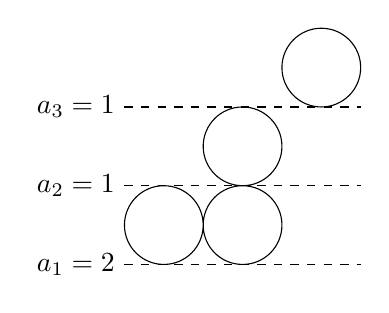
\begin{tikzpicture}[baseline]
    \draw [dashed] (0,0) node [left] {$a_1 = 2$} --++ (3,0);
    \draw [dashed] (0,1) node [left] {$a_2 = 1$} --++ (3,0);
    \draw [dashed] (0,2) node [left] {$a_3 = 1$} --++ (3,0);
    \draw (.5,.5) circle (.5) (1.5,.5) circle (.5) (1.5,1.5) circle (.5) (2.5,2.5) circle (.5);
  \end{tikzpicture}
  \]
  or another distribution
  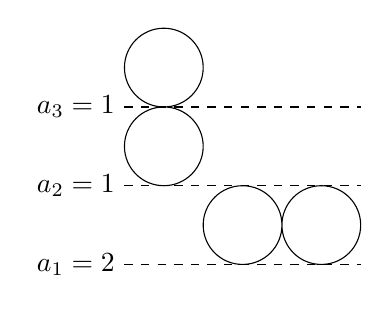
\begin{tikzpicture}[baseline]
    \draw [dashed] (0,0) node [left] {$a_1 = 2$} --++ (3,0);
    \draw [dashed] (0,1) node [left] {$a_2 = 1$} --++ (3,0);
    \draw [dashed] (0,2) node [left] {$a_3 = 1$} --++ (3,0);
    \draw (1.5,.5) circle (.5) (2.5,.5) circle (.5) (.5,1.5) circle (.5) (.5,2.5) circle (.5);
  \end{tikzpicture}

  能级 \quad 能极简并度
  \item  对孤立子
  \[\sum_\alpha a_\alpha = N, \sum_\alpha \epsilon_\alpha a_\alpha = E\]
  \item 对一个给定的 $\{a_\alpha\}$, 可以有不同的量子态. $\Rightarrow W(\{a_\alpha\})$
  等几率原理 $\{a_\alpha\}$ 出现的几率 $\propto$ $W\{a_\alpha\}$.
\end{itemize}

如果可区分 $W(\{a_\alpha\}) = \frac{N!}{\prod_\alpha a_\alpha!} \prod_\alpha g_\alpha^{a_\alpha}$,
Fermion $W_F(\{a_\alpha\}) = \prod_\alpha \frac{g_\alpha!}{a_\alpha!(g_\alpha - a_\alpha)!}$,
Boson $W_B(\{a_\alpha\}) = \prod_\alpha \frac{(g_\alpha + a_\alpha - 1)}{a_\alpha!(g_\alpha - 1)!}$.

\chapter{Microregular Ensemble}

平衡态统计一般理论是系综理论. 适用范围:宏观多粒子系统.

系综:微正则系综(基本系综),正则系综,巨正则系综.
\begin{itemize}
  \item 微正则系综:$E$, $N$, $V$ 固定
  \item 正则系综:$T$, $N$, $V$ 固定
  \item 巨正则系综:$T$, $\mu$, $V$ 固定
\end{itemize}

\section{经典统计系综}

经典力学的微观状态:相空间中一个点 $(q,p)$ 满足正则运动方程
\begin{equation}
  \dot q_i = \pdv H{p_i},~ \dot p_i = -\pdv H{q_i}, ~ i = 1,\ \ldots\,,~s
\end{equation}
$\{(q_n(t), p_n(t))\}$
相轨道 $(\dot q_i(t), \dot p_i(t))$,轨道上任意一点 $\d\Omega = \prod_i \d q_i \d p_i$, $i = 1$, $\ldots\,$,~$s$.

设 $\Gamma$ 为给定宏观物理条件下所有可能的微观状态 $\tilde\rho \d\Omega$:
$\d\Omega$ 内的微观状态数,则 $\rho \d\Omega = \frac{\tilde\rho \d\Omega}\Gamma = \frac{\tilde\rho \d\Omega}{\int \tilde\rho \d\Omega}$ 是某微观状态出现在 $\d\Omega$ 内的几率,满足归一化 $\int \rho \d\Omega = 1$,$\rho$ 为几率密度.

任何物理可观测量 $O$ 是微观力学量 $O$ 的统计平均.
\begin{equation}
  \overline O = \int \d\Omega\rho O
\end{equation}
\begin{itemize}
  \item 系统处于某一微观状态 $\leftrightharpoons$ 处于该微观状态的系统
  \item 处于 $\d\Omega$ 中的系统是 $\tilde \rho \d\Omega$ 个 $\Gamma$ 个系统的集合称为一个统计系综.
  \item 系综是假想的和所研究系统性质完全相同的彼此独立、各自处于某一微观状态的大量系统的集合.
\end{itemize}

\section{系综所满足的方程:Liouville 定理}

\begin{theorem}[Liouville 定理]
  系综的几率密度 $\rho$ 在运动中不变,
  \[\odv \rho t = 0, ~ \odv{\tilde\rho}t = 0.\]
  代表点数守恒
\begin{equation}
  \pdv\rho t + \nabla \bm J_\rho = 0,~ \bm J_\rho = \rho \bm r,
  \nabla = \ab(\pdv*{}{q_i},\pdv*{}{p_i}),~ \bm v = \sum_i (\dot q_i, \dot p_i)
\end{equation}
\begin{equation}
  \odv{\tilde\rho}t = \pdv{\tilde\rho}t + \sum_i \bm r_i (\rho\bm r_i \bm r_i)
= \pdv{\tilde\rho}t + \sum_i \ab(\pdv{\tilde p}q_i\dot q_i + \pdv{\tilde p}p_i\dot p_i)
= -\tilde\rho \sum_i \ab\{\pdv H{q_i,p_j} - \pdv H{p_i,q_j}\} = 0
\end{equation}
最后得出 Liouville 方程
\begin{equation}
  \pdv{\tilde\rho}t + \{\tilde\rho,\rho\} = 0
\end{equation}
\end{theorem}

\section{量子统计系综}

\begin{itemize}
  \item 对量子力学系统,我们用波函数 $\psi_n$ 或态 $\ket|n>$ 来代替相空间的 $(q,p)$
  \item $A_n = \braket<n|\hat A|n>$
  \item 统计系综,考虑一系列的态 $\ket|1>$, $\ket|2>$, $\ldots\,$,~$\ket|n>$.
  \item 第 $n$ 个态有 $\tilde \rho_n$ 个简并度,即有 $\tilde\rho_n$ 个系统.
\end{itemize}

总系统数 $N = \sum_n \tilde \rho_n$

$\rho_n = \frac{\tilde\rho_N}{N}$ 处于第 $n$ 个态的几率

$\sum_n \rho_n = 1$, $\overline A = \braket<A> = \sum_n \rho_n A_n$

统计算符(密度矩阵) $\hat \rho = \sum_n \ket|n> \rho_n \bra<n|$

$\{\ket|i>\}$ 一套正交\footnote{即 $\delta\braket<i|j> = \delta_{ij}$}完备\footnote{即 $\sum_i \ketbra|i><i| = \mathbbm 1$: 对于 $\{\ket|0>m \ket|\uparrow>, \ket|\downarrow>, \ket|\uparrow\downarrow>\}$,存在 $\ketbra|0><0| + \ketbra|\uparrow><\uparrow| + \ketbra|\downarrow><\downarrow| + \ketbra|\uparrow\downarrow><\uparrow\downarrow| = \mathbbm 1$}基.

密度矩阵
\begin{equation}
  \rho_{ij} = \braket<i|\hat\rho|j> = \sum_n \braket<i|n> \rho_n \braket<n|j>
\end{equation}
\[
  A_{ij} = \braket<i|A|j>,~ \overline A = \sum_n \rho_n \braket<n|A|n> = \sum_{ij} \sum_n \rho_n \braket<n|j> \braket<j|A|i>\braket<i|n> = \sum_{ij} \rho_{ij}A_{ji} = \Tr (\hat \rho A)
\]
\[\Tr \sum_i \rho_{ii} = 1\]

$\hat\rho$, $\ket|n>$ Schr\"odinger eq
\begin{equation}
  \iu\pdv*{}t \ket|n> = \hat H\ket|n>
\end{equation}
\[
  \iu \pdv*{}t \hat\rho = \sum_n \ab[\ab(\iu\pdv*{}t\ket|n>)\rho_n\bra<n| - \ket|n>\rho_n\ab(-\iu\pdv*{}t\bra<n|)]
  = \sum_n H\ket|n> \rho_n\bra<n| - \ket|n>\rho_n\bra<n| H = H\hat\rho - \hat\rho H = [H,\hat\rho]
\]
Finally, we have
\begin{equation}
  \pdv*{}t\hat\rho + \iu[H,\hat p] = 0
\end{equation}
即 $\hat\rho$ 的 Heisenberg eq. of motion.

\section{微正则系综}

\begin{itemize}
  \item 经典微正则系综:$E$, $N$, $V$ 不变系综 --- 孤立系.
\end{itemize}
由 Liouville 定理
\[\odv\rho t = 0\]
若在平衡态物理量不随时间变化,就要求在相空间固定点,$\rho$ 不随时间变化,即必要条件 $\pdv \rho t = 0$.
$\Longrightarrow$ 在相轨道内 $\rho$ 为常数.

但 Liouville 定理和平衡态物理量不变不能保证不同轨道的 $\rho$ 相同.

微正则系综的基本假设
\begin{itemize}
  \item 当 $H(q,p) = E$ 时,$\rho$ 是常数,即相空间中的等能面.
  \item 当 $H(q,p) \neq E$ 时(存在集合 $\{p,q\}$),$\rho = 0$.
\end{itemize}
To summarize
\begin{equation}
  \rho =
  \begin{cases}
    C & E \leq H \leq E + \Delta E,\\
    0 & otherwise
  \end{cases}
\end{equation}
守恒条件 (Normalization of $\rho$)
\begin{equation}
  \lim_{\Delta \to 0} C \int_{\Delta E} \d\Omega = 1.
\end{equation}
The mean value
\begin{equation}
  \overline O = \lim_{\Delta E \to 0} C \int_{\Delta O \d \Omega}.
\end{equation}
量子微正则系综
\begin{equation}
  H(q,p) \longrightarrow E_n
\end{equation}
加入
\begin{enumerate}
  \item 粒子的全同性
  \item $\rho_n =
  \begin{cases}
    C, & E_n = E\\
    0, & E_n \neq E
  \end{cases}$,$n$ 为标记量子态的量子数.
  $\sum_{n(E_n=E)} \rho_n = C$ ($\sum_{n(E_n=E)} 1 = 1$).
\end{enumerate}
\[
  \mathcal N(E,V,N) = \sum_{n(E_n=E)} 1, ~ C = \frac{1}{\mathcal N(E,N,V)}
\]
\chapter{From Microcanonical Ensembles to Canonical Ensembles}

\begin{definition}[正则系综]
  系统与大热源接触,达到平衡的系综,$(T,V,N)$ 固定.
\end{definition}

大热源的作用是提供确定的温度
\begin{itemize}
  \item $A$: 就是要研究的正则系综中的系统.
  \item $B$: 大热源中的系统
  \item $A + B$: 孤立系.
\end{itemize}
\[
  E_\text{total} = E_A + E_B,~ V_\text{total} = V_A + V_B,~
  N_\text{total} = N_A + N_B
\]
Assume $\Omega(E_\text{total})$ is the number of the total state of $A + B$,
then the states in $A$ is labelled as $\ket|n>$, and $A$ is at the $|n>$ state;
$B$ has $\Omega(E_\text{total} - E_A)$ states. The probability that the system $A$ at state $\ket|n>$ can be described as
\begin{equation}
  \rho_{An} = \frac{\Omega_B(E_\text{total} - E_A)}{\Omega(E_\text{total})}.
\end{equation}
and the mean value $\bar E_n \ll E_\text{total}$, $E_A \ll E_\text{total}$.
It's not important that which state $B$ is located, as well as $B$'s properties.
Then, the freedom-particle system can be used to represent $B$.
\begin{example}[Chapter 3, Problem 1]
  $\Omega_B(E_\text{total} - E_A) \sim (E_\text{total} - E_A)^M$,
  $M \sim O(N_3) \sim O(N)$.
  To expand it:
  \[
    \Omega_B(E_\text{total} - E_A) = E_\text{total}^M\ab(1 - \frac{E_A}{E_\text{total}})^M = E_\text{total}^M\ab(1 - M\frac{E_A}{E_\text{total}} + \cdots)
  \]
  we can also expand it in another way (a safer expansion)
  \[
    \Omega_B(E_\text{total} - E_A) = \exp[M \ln(E_\text{total} - E_A)]
  \]
  Then expand the ``$\ln$'' item
  \[
    \ln(E_\text{total} - E_A) = \ln E_\text{total}
  + \ln\ab(1 - \frac{E}{E_\text{total}}) = \ln E_\text{total} - \frac{E_A}{E} - \frac12\ab(\frac{E_A}{E_\text{total}})^2 + \cdots
  \]
  then we have
  \[
    \rho_{An} = \frac{1}{\Omega(E_\text{total})}\upe^{\ln\Omega_B}
  = \frac{1}{\Omega(E_\text{total})} \exp\ab[\ln\Omega_B(E_\text{total}) - \pdv{\Omega_B(E_B)}{E_\text{total}}E_A + \cdots]
  \approx \frac{\Omega_B(E_\text{total})}{\Omega(E_\text{total})} \upe^{-\beta E_A}
  \equiv \frac1{Z_N}\upe^{-\beta E_A}
  \]
  we define $\beta = \pdv{\Omega_B(E_\text{total})}{E_\text{total}} \xlongequal{\triangle} \frac1{k_BT}$
  then remove the ``$A$'' index
  \[
    \rho_{An} = \rho_n,~ \sum_n \rho_n = 1 \Rightarrow Z_N = \sum_n \upe^{-\beta E_N}
  \]
  Now, we arrive at the partition function $Z_N$
  \begin{equation}
    Z_N = \Tr\upe^{-\beta H} = \sum_n \braket<n|\upe^{-\beta H}|n> = \sum_n \upe^{-\beta E_n}
  \end{equation}
\end{example}
Using the partition function, we have
\begin{gather}
  \overline A = \sum_n A_n \rho _n = \frac1{Z_n} \sum_n \braket<n|A|n> \upe^{-\beta E_n}
  = \frac1{Z_n} \sum_n \braket<n|A \upe^{-\beta H}|n> = \frac1{Z_n} \Tr A\upe^{-\beta H}.\\
  \bar E \xlongequal{\text{inner energy}} \sum_n E_n\rho_n
  = \frac1{Z_n} \sum_n E_n \upe^{-\beta E_n}
  = \frac1{Z_n} \ab(-\pdv*{}\beta \sum_n \upe^{-\beta E_n})
  = -\frac1{Z_n} \pdv*{}p Z_n = -\pdv*{}\beta \ln Z_n\\
  p_n = -\pdv{E_n}V,~
  \overline p = \sum_n p_n \rho_n = \frac1{Z_n} \sum_n -\pdv{E_n}V \upe^{-\beta E_n} = \frac1\beta \pdv*{}V \ln Z_N\\
  \d S = \frac{\d \bar E}T + \frac{\overline p}T \d N
  = k_B(\beta\d \bar E + \beta\overline p\d V)
  = k_B\ab(-\beta\pdv*{}\beta \d\ln Z_N + \d V\pdv*{}{V}\ln Z_N)
  = \d\ab[k_B \ab(\ln Z_N - \beta \pdv*{}p \ln Z_N)]\\
  F = \bar E - TS = -k_B T \ln Z_N
\end{gather}

\section{能量涨落,热力学极限,经典极限}

\begin{definition}[涨落]
  For energy:
  \begin{enumext}[columns = 2]
    \item 方差:$\frac{\overline{(E - \bar E)^2}}{E^2}$
    \item 方均根:$\sqrt{\frac{\overline{(E - \bar E)^2}}{E^2}}$
  \end{enumext}
  \[
    \overline{(E - \bar E)^2} = \overline{(E^2 - 2E\bar E = \bar E^2)} = \overline{E^2} - \bar E^2,~
    \overline{E^2} = \sum_n E_n^2 \rho_n = \ldots = \bar E^2 - \pdv {\bar E}\beta\bigg|_{N,V}
  \]
  \[\overline{(E - \bar E)^2} = -\pdv{\bar E}\beta\bigg|_{N,V} = k_BT\ab(\pdv{\bar E}T)_{N,V} = k_BT^2C_V\]
  \[
    \frac{\sqrt{\overline{(E-\bar E)^2}}}{\bar E}
  = \frac{\sqrt{k_B+C_V}}{\bar E}
  = \frac{\sqrt{k_Bc_v}+\sqrt N}{A+N} \propto \frac1{\sqrt N}
  \]
\end{definition}

\begin{definition}[热力学极限]
  $N$, $V \to \infty$, $n = \frac NV$ final.
\end{definition}
\begin{definition}[经典极限]
  热波长 $\lambda_T = h/()2\pi m k_B T^{1/2} \ll \delta\bar r$ (average distance of particle).

  $\Delta E = E_n - E_{n-1} \ll k_BT$ --- 经典极限.

  \[
    Z_n = \frac1{N!h^3} \int \d\Omega \upe^{-\beta H(q,p)}
  \]
\end{definition}

\section{State equation of non-ideal gas}

Model:
\begin{equation}
  E = k + V = \sum_{i = 1}^N \frac{\bm p_i^2}{2m} = \sum_{i<j}\phi_{ij}
\end{equation}
here, $\phi_{ij} = \phi(\bm r_i - \bm r_j)$ stands for the interactions between molecule.
\[
  Z_N = \int (\d\Omega) \upe^{-\beta(k+V)},~
  (\d\Omega) = \frac{1}{N!h^{3N}}\prod_i\d^3p_i\d^3r_i
  = \frac{1}{N!\lambda_T^{3N}} Q_N(\beta,V)
\]
while $Q_N = \int \d\bm r_1 \cdots \bm r_N \upe^{-\beta\sum_{i<j}\phi_{ij}} = \int (\d\bm r) \prod_{i<j} \upe^{-\beta \phi_{ij}}$.

For ideal gas, $Q_N = V^N$. The interacting force is graphed:
$r^* \sim 1\text\AA$

\[  
  f_{ij} = e^{-\beta p_{ij}} - 1
\]
\[
  f(r) =
  \begin{cases}
    -1, & r \to 0, (\phi \to \infty)\\
    0, & r \to r^* (\phi \to 0)
  \end{cases}
\]
\[
  Q_N = \int (\d\bm r) \prod_{i<j} (1 + f_{ij}) = \int (\bm \d r) \ab(1 + \sum_{i<j}f_{ij} + \sum_{i<j}f_{ij}\sum_{i'<j'}f_{i'j'} + \cdots)
\]
Since $\upe^{-\beta\phi(r_0)}/2 \ll 1$,
\[  
Q_N = \int (\d \bm r) (1+ \sum_{i<j}f_{ij})
= V^N + \frac12 N(N-1) V^{N-2} \int \d\bm r_1 \d\bm r_2 f_{12},~
\bm r_1 - r_2 = \bm r
\]
\[
  \int \d\bm r,\d\bm r_2 f_{12} = \int \d\bm r_1 \int\d\bm r_2 f(|\bm r|) \approx V\int \d r f(r)
\]
\[
  Q_N \approx V^N\ab(1 + f\frac12(N^2 - N))/V \int \d^3\bm r f(r)
  \approx V^N \ab(1 + \frac12 \frac{N^2}V \int \d\bm r f(r))
\]
\[
  \ln Q_N = N\ln V + \ln\ab(1 + \frac{N^2}{2V} \int\d^3\bm r f(r))
\]
The pressure
\[  
  p = \frac1\beta \pdv*{}V \ln N_N = \frac1\beta \pdv*{}V\ln Q_N
    = \frac{Nk_BT}V\ab[1 \underset{B_2/N}{\text{\fbox{$- \frac N{2V^2} \int \d^3r f(\bm r)$}}}]
\]
\[
  \phi(r) = 
  \begin{cases}
    \infty, & r < r_0\\
    -p_0\ab(\frac{r_0}{r})^b, & r \geq r_0
  \end{cases}
\]
\[
  B_2 = -\frac N2 \int_0^\infty \exp\ab(-\frac{-\phi(r)}{k_BT}-1) r^2 \d r
  \approx 2\pi N\ab(\frac{r_0^3}{3} - \phi_0\frac{r_0^3}{3k_BT})
  \equiv N_b - \frac{Na}{k_BT}
\]
Substitute $B_2$ into $p$
\[
  p = \frac{Nk_BT}{V}\ab(1 + \frac{Nb}{V}) - \frac{N^2a}{V^2} \approx \frac{Nk_BT}{V(1-Nb/V)} - \frac{N^2a}{V^2}
\]
Then we arrive at the 范德瓦耳斯 equation
\begin{equation}
  \ab(p + \frac{N^2a}{V^2})(V - Nb) = N k_B T
\end{equation}
\chapter{Grand Canonical Ensemble}

$(T, \mu, V)$ 不变.

\begin{itemize}
  \item 与正则系综类似,热库同时也是粒子源.
  \begin{equation}
    E_T = E_A + E_B, ~ N_T = N_A + N_B
  \end{equation}
  \begin{align*}
    \rho_n & = \rho_{AN} = \frac{\Omega_B(N_T - N_A, E_T - E_A)}{\Omega(N_T,E_T)}
    = \frac1{\Omega(N_T,E_T)} \upe^{\ln \Omega_B (N_T-N_B, E_T-E_B)}\\
  & = \frac{\Omega_3(N_T,E_T)}{\Omega(N_T,E_T)}
  \exp\ab[-\pdv{\ln\Omega_B(N_T,E_T )}{{N_T}} N_A - \pdv{\ln\Omega_B(N_T,E_T )}{{N_T}} N_A]\\
  & = \frac1{Z_G} \upe^{\beta \mu N_A-\beta E_A}
  \end{align*}
  即 $\rho_{N_A} = \frac1{Z_G} \upe^{-\beta(E_n - \mu_N)}$.
  The normalization condition
  \[
    \sum_{N=0}^\infty \sum_n \rho_{Nn} = 1
  \]
  \[
    Z_G = \sum_{N=0}^\infty \upe^{\beta\mu N} \sum_n \upe^{-\beta E_N}
  = \sum_{N=0}^\infty \upe^{\beta\mu N} Z_N = \Tr \upe^{-\beta(\hat H - \mu N)}
  \]
  while $\mu$ is fermion's erergy.
  \[
    \braket<n|\hat H|n> = E_n
  \]
  \begin{align}
    \bar E & = -\pdv*{}\beta \ln Z_G\\
    p & = \frac1\beta \pdv*{}V \ln Z_G\\
    S & = o_B(\ln Z_G - \alpha \pdv*{}\alpha \ln Z_G - \beta \pdv*{}\beta \ln Z_G)\\
    F & = -k_BT\ln Z_G + k_BT \alpha \pdv*{}\alpha \ln Z_G\\
    \psi & = -k_B T \ln Z_G
  \end{align}
  \item 经典和粒子数涨落 $\sim \frac1{\sqrt N}$.
  \item 经典极限 $Z_G = \sum_N \upe^{-\alpha N} Z_N$
\end{itemize}

\begin{example}[固体表面的吸附率]
  \[\theta = \frac{\overline N}{N_0}, ~ N \to \bar N\]
  $(T,\mu, \nu)$
  单个分子被吸附后的能量降低 $\epsilon_0$.
  \[
    E_N = -\epsilon_0 N
  \]
\end{example}
\[
  Z_G = \sum_{N=0}^{N_0} \sum_n \upe^{-\alpha N-\beta E_N}
= \sum_{N=9}^{N_0} \sum_n \upe^{-\alpha N-\beta E_N}
= \sum_{N=0}^\infty \sum_n \upe^{\beta(\beta+\epsilon_0)N}
\]
其中 $n$ 表示分子占据 $N$ 个确定吸附中心中的 $N$ 个时的某一特定状态
\[
  \sum_n= \frac{N_0!}{N!(N_0 - N)}!
\]
\[
  Z(G) = \sum_{N=0}^{N_0} \frac{N_0!}{N!(N_0-1)!} \upe^{p(\mu+\epsilon_0)N}
= (1 + x)A^{N_0} = (1 + \upe^{\beta(\mu + \epsilon_0)})^{N_0}
\]
\[
  \overline N = -\pdv*{}x \ln Z_G
= \frac1\beta \pdv*{}\mu \ln Z_G\big|_{T_{\beta(\mu+\epsilon_0)}}
= N_0 \pdv*{}\alpha \upe^{\alpha+\beta_0\epsilon}
= \frac{N_0\upe^{\beta(\mu+\epsilon_0)}}{1 + \upe^{\beta(\mu+\epsilon_0)}}
\]
这里达到平衡态 $\mu = \mu_A = \mu_B$, 这里 $\mu_B$ 可以用理想气体的化学势.
\[
  \upe^{-\beta\mu} = \frac{(2\pi mk_BT)^{3/2} k_BT}{\beta h^3}
\]
\[
  \theta = \frac{\bar N}{N_0}
= \frac{ph^3}{ph^3 + (2\pi m)^{3/2} - (k_BT)^{5/2} - \upe^{-\epsilon_0/k_BT}}
\]
即 $p$ 升高,$\theta$ 升高;$T$ 升高;$\theta$ 下降.
\chapter{Quantum Statistics}

\begin{itemize}
  \item For dimension $d = 3$: Quantum gas could be either boson or fermion
  \item For dimension $d = 2$: Quantum gas could be either boson, or fermion, or anyon.
  \item For dimension $d = 1$: The statistic properties are related to interactions.
\end{itemize}

\section{Bose and Fermi Statistics of free particles under GRSC}

The Giant Regular System Comprehensive is
\begin{equation}
  Z_G = \sum_{N=0}^\infty \sum_{s~\text{$N$ is fixed}}
        \upe^{-\alpha N-\beta E_s}
\end{equation}
Combine $E_{N_{n_1}} = E_{N_{n_2}} = \ldots = E_N$ together and
substitute them into $Z_G$
\[
  Z_g = \sum_{N=0}^\infty \sum_{E_N} \sum_{s(E_{N_s}=E_N)}
    \upe^{-\alpha N-\beta E_{N_s}}
\]
For free particles
\[
  E_N = \sum_\lambda a_\lambda \epsilon_\lambda, \qq{and}
  N = \sum_\lambda a_\lambda
\]
$\epsilon_\lambda$ is the energy of single particle,
$a_\lambda$ is the occupation number of $\lambda$ energy level,
and $\{a_\lambda\}$ is a distribution of the number of particles
after a given $\lambda$.
Now, we can sum in partition
\[
  Z_a = \sum_{N=0}^\infty \sum_{E_N}
  \sum_{\{a_\lambda|\sum_\lambda a\lambda \epsilon_\lambda = E_N\}}
  W(\{a_\lambda\})
  \upe^{-\sum_\lambda (\alpha+\beta\epsilon_\lambda)a_\lambda}
= \sum_{\{a_\lambda\}} W(\{a_\lambda\})
  \upe^{-\sum_\lambda (\alpha+\beta\epsilon_\lambda)a_\lambda}
\]
Here, $\{a_\lambda\}$ represent various energy level and particle numbers;
$W$ is the micro state number of distributing $\{a_\lambda\}$. Hence
\[
  Z_a = \sum_{\{a_\lambda\}} \prod_\lambda W_\lambda
  \upe^{-\alpha a_\lambda -\beta a_\lambda \epsilon_\lambda}
= \prod_\lambda \ab(\sum_{a_\lambda}) W_\lambda
  \upe^{-\alpha a_\lambda-\beta a_\lambda\epsilon_\lambda}
\]
For Fermion, a state can only contain one particle
\[
  W_\lambda = \frac{g_\lambda!}{a_\lambda!(g_\lambda-a_\lambda)},
\]
here, $g_\lambda$ is the degeneracy number.
For Boson,
\[
  W_\lambda = \frac{(g_\lambda + a_{\lambda-1})!}{a_\lambda!(g_\lambda - 1)!}
\]
Substitute $W$ respectively
\begin{gather}
  Z_\lambda^{(F)} = \sum_{a_\lambda=0}^\infty
  \frac{g_\lambda!}{a_\lambda!(g_\lambda - 1)!}
  \upe^{-(\alpha+\beta\epsilon_\lambda)a_\lambda}
= (1 + \upe^{-\alpha - \beta\epsilon_\lambda})^{-g_\lambda}\\
  Z_\lambda^{(B)} = \sum_{a_\lambda=0}^\infty
  \frac{(g_\lambda + a_\lambda - 1)!}{a_\lambda!(g_\lambda - 1)!}
  \upe^{-(\alpha+\beta\epsilon_\lambda)a_\lambda}
= (1 - \upe^{-\alpha - \beta\epsilon_\lambda})^{-g_\lambda}
\end{gather}
Combine $Z_\lambda^{(F)}$ and $Z_\lambda^{(B)}$ together,
\[
  Z_G = \prod_\lambda Z_\lambda =
  \prod_\lambda (1 \pm \upe^{-\alpha-\beta\epsilon_\lambda})^{\pm g_\lambda}
\]
\[
  \ln Z_G = \pm \sum_\lambda g_\lambda
  \ln(1 \pm \upe^{-\alpha-\beta\epsilon_\lambda})
\]
Now, calculating the average distribution
(assume that $\xi$ is a given energy level)
\begin{align*}
  \bar a_\xi & = \sum_N \sum_n a_\xi \rho_{N\xi}
= \frac1{Z_G} \sum_{G_\xi} a_\xi W_\xi \upe^{-(\alpha+\beta\epsilon_\xi)a_\xi}
= \frac1{Z_\xi} \sum_{a_\xi} a_\xi W_\xi \upe^{-(\alpha+\beta\epsilon_\xi)a_\xi}\\
& = -\frac1{Z_\xi} \pdv*{}\alpha Z_\xi = -\pdv*{}\alpha \ln Z_\xi
  = -\pdv*{}\alpha(\pm g_\xi \ln(1 \pm \upe^{-\alpha-\beta\epsilon_\xi}))
= \frac{g_3}{\upe^{\beta(\epsilon_\xi-\mu) \pm 1}}
\end{align*}

\section{The Symmetry of Quantum Statistic \& Wave Function}

For example, a wave function contains $N$-particle
\[
  \psi(\bm r_1,\cdots,\bm r_N)
\]
If $\bm r_i \leftrightarrow \bm r_j$, then
\[
  |\psi(\cdots,\bm r_i,\cdots,\bm r_j,\cdots)|^2 =
  |\psi(\cdots,\bm r_j,\cdots,\bm r_i,\cdots)|^2
\]
then
\[
  \psi(\bm r_2,\bm r_1,\cdots) =
  \upe^{\iu \alpha_{12}} \psi(\bm r_1,\bm r_2,\cdots)
\]
For Fermion, due to paul's principle, $\psi(\bm r_1,\bm r_1,\bm r_3) = 0$.
\[
  \lim_{\bm r_2\to\bm r_1} \psi(\bm r_1,\bm r_2,\bm r_3,\cdots) = 0
\]
and $\psi(\bm r_1,\bm r_2,\cdots) = -\psi(\bm r_2,\bm r_1,\cdots)$.
Since $\upe^{i\pi} = -1$, then $\alpha_{12} = \pi \pm 2n\pi$.

For Boson,
\[
  \lim_{\bm r_1 \to \bm r_2} \psi(\bm r_1, \bm r_2, \cdots)
= \lim_{\bm r2 \to \bm r_1} \psi(\bm r_2, \bm r_1, \cdots)
= \psi(\bm r_1,\bm r_1,\cdots) \neq 0
\]
then we have $\alpha_{12} = \pm 2n\pi$.

In 3D space, rotate the particle
$\bm r_2$ rotate around $\bm r_1$ has no topo barrier.
$\upe^{\iu \phi} = \upe^{\iu 2\pi n}$. If n is $odd$, then it's Fermion; or it is Boson.

In the space's dimension greater or equal than $3$, only exist Bose or Fermi statistic.

\section{Anyon (任意子), Braid Group (辨子群)}

$\tau \in (0,\beta)$, then 
\[
  \rho(x,x';t) = \int_{(x)}^{(x')} \D x
  \upe^{-\iu \int_0^\infty \d t \mathcal L}
\]
where $\D$ means integral by all the paths.

In 3D space, path 1 is equivalent to path 2, since it could transform between two paths without break by the propagator; but when the paths are limited with  in 2D space, it could not transform from path 1 to path 2 continuously. Now,
\[
  \D x \to \sum_\alpha \varphi_\alpha \D x_\alpha
\]
where $\alpha$ is used to label the 有可相互连续互变的等价 in 2D space..
Since the integral is not related to the length of the path, $\varphi_\alpha$ is a phase factor $\upe^{\iu\theta}$, in which $|\varphi_\alpha| = 1$.

If there are $N$ particles in a 2D space, that is
\[
  R^{2N} = \{\bm r_1, \cdots, \bm r_N\} = M_N \text{(多连通)}
\]
and there many paths that form different 等价类 $\{\alpha\}$.

For N particles, the process of braiding form group. $B_M(\mathbb R^2)$: braid group, for example (2D) [!Figure]
\begin{enumext}[label = (\alph*), columns = 3]
  \item $x_i x_{i+1} = \sigma_i$
  \item $\sigma_i \sigma_{i+1} \sigma_i = \sigma_{i+1} \sigma_i \sigma_{i+1}$.
  \item $x_{i+1} x_i = \sigma_i^{-1}$.
\end{enumext}
then, $\sigma_i \sigma_i^{-1} = 1$.
and $\sigma_i \sigma_k = \sigma_k \sigma_i$, where $k \neq i \pm 1$.
also 3D. [!Figure]
(1) -- (3) are the relation that a braid group needs to satisfy.

Non-abelian group.

The expression of Braid group:
\[
  \varphi_\theta(\sigma_i) = \upe^{-\iu\theta}, \quad (0 \leq \theta < 2\pi)
\]
\begin{enumext}[label = (\alph*)]
  \item $\theta = 0$, identity rep \textrightarrow Boson
  \item $\theta = \pi$, $Z_L$ rep \textrightarrow Fermion
  \item $\theta = \text{rational}$ \textrightarrow Fractional statistics Anyon.
\end{enumext}
Exchange: $r_i r_{i+1}$, rotate: $r_i r_{i+1} r_i$, then move $r_{i+1} r_i$.
That is
\begin{equation}
  \varphi_\theta (\sigma_i^{\pm1}) = \upe^{\mp\iu\theta} = \upe^{-\iu\frac\theta\pi (\pm\pi)}
= \exp\ab[-\iu \frac\theta\pi \sum_{l<j} \Delta\phi_{lj}]
\end{equation}
where, only $\Delta\phi_{i,i+1} = \pm\pi$, and $\Delta\phi_{lj} = 0$.

For normal $\alpha$,
\begin{equation}
  \varphi_\theta(\alpha)
= \exp\ab(-\iu\frac\theta\pi \int \d t \odv*{\sum_{i<j} \phi_{ij}}t)
\end{equation}
(? extra factor $\sum_\alpha \varphi_\alpha \D \mathcal L$)
For the original propagator,
\[
  K(r't';rt) = \int \D r \exp\ab\{\iu \int_t^{t'} \d t \ab(\mathcal L - \frac\theta\pi \odv*{\sum_{i<j} \phi_{ij}}t)\}
\]
then
\begin{equation}
  \psi(r't') = \int \D r K^{(0)} (r't',rt) \psi(r,t)
\end{equation}
Now, define
\begin{equation}
  \tilde\psi(rt) = \exp\ab\{-\iu \frac\theta\pi \int_r^{r^0 \d\ab(\sum_{i<j} \phi_{ij})}\} \psi(r,t)
\end{equation}
where $r^0$ is some ref point.
After considering braiding
\begin{gather}
  \tilde\psi(r't') = \int \D rK(r't',rt) \tilde\psi(rt)\\
  \tilde\psi(r,t)  = \prod_{i<j} \frac{(z_i - z_j)^{\theta/\pi}}{|z_i - z_j|^{\theta/\pi}} \psi(r,t)
= \prod_{i<j} (z_i - z_j)^{\theta/\pi} f(\theta,t)
\end{gather}
where $f(\theta)$ is the exchange pair.
If the two particles exchanged, then it will lead to a factor
\[
  (-1)^{\theta/\pi} = \upe^{\iu \frac\theta\pi \pi} = \upe^{\iu\theta}
\]
that is a phase of $\exp\ab(\iu\frac\theta\pi \arg(z_i - z_j))$.

\subsection{Non-Abelian Statistics}

If the wave function is $s$ order degeneracy at a certain energy level, then for
\[
  \{\psi_i(\bm r_1, \ldots, \bm r_N), \ldots, \psi_s(\bm r_1, \ldots, \bm r_N)\}
\]
if we switch $\bm r_i \leftrightarrow r_j$, it will lead
\[
  \psi_a(\bm r_1, \ldots, \bm r_j, \bm r_i, \ldots, \bm r_N)
= \sum B_{ab} \psi_b(\bm r_1, \ldots, \bm r_i, \bm r_j, \ldots, \bm r_N)
\]
where $B_{ab}$ is a matrix. Write it into matrix equation form
\begin{equation}
  \begin{pmatrix}
    \psi_1\\\vdots\\\psi_s
  \end{pmatrix}_{\bm r_j, \bm r_i} =
  \pxmat[showleft = 2, showtop = 2] Bss
  \begin{pmatrix}
    \psi_1\\\vdots\\\psi_s
  \end{pmatrix}_{\bm r_i, \bm r_j}
\end{equation}
obviously, $B_{ij} B_{jk} \neq B_{jk} B_{ij}$,
which is the non-Abelian representation. of braid group.
\fbox{Tops Quan Computational}

\section{1D Statistics: Interaction Corresponding}

For $N$ particles with $G$ states, how to promote Bose or Fermi Statistics.
\begin{align}
  W_B & = \frac{[G + N - 1]!}{N! (G - 1)!},\\
  W_F & = \frac{G!}{N! (G - 1)!},\\
\end{align}
when $0 \leq s \leq 1$,
\[
  W_s = \frac{[G + (N - 1)(1 - S)]!}{N![G - SN - (1 - S)]!}
\]
For a set of $N$: $\{N_x\}$, existing $\alpha$ to satisfy
\begin{equation}
  W = \prod_\alpha \frac{[G_\alpha + N_\alpha - 1 - \sum_{\beta \neq \alpha} S_{\alpha\beta} (N_\alpha - \delta_{\alpha\beta})!]}
  {N_{\alpha!}[G_\alpha - 1 - \sum_\beta S_{\alpha\beta} (N_\alpha - \delta_{\alpha})]!},
\end{equation}
let $S_{\alpha} = s\delta_{\alpha\beta}$,
\begin{enumext}[label = \roman*, columns = 2]
  \item $S = 0$
  \begin{equation}
    W_B = \prod_\alpha \frac{(G_\alpha + N_\alpha - 1)!}{N_\alpha(G_\alpha - 1)}
  \end{equation}
  \item $S = 1$
  \begin{equation}
    W_F = \prod_\alpha \frac{G_\alpha!}{N_\alpha!(G_\alpha - 1)!}
  \end{equation}
\end{enumext}
\begin{example}
  $\delta$-interaction Boson (Yang-Yang).
  For 1D, the Hamiltonian is
  \[
    H = -\sum_{i=1}^N \pdv*[2]{}{x_i}
      + 2C \sum_{i<j} \delta(x_i - x_j),
    \quad c \geq 0
  \]
  Apply the Periodic Boundary Conditions, we can have the strict solution.
  Due to the translation conservation, apply the Fourier transformation
  \[
    E = \sum_n K_i^2
  \]
  while the continuous limitation
  \[
    S_{\alpha\beta} \to S(k,k') = \delta(k - k') + \frac1{2\pi} \odv*{\theta(k - k')}k
  \]
  that is
  \[
    \odv{\theta(k - k')}k = -\frac{2C}{C^2 + (k - k')^2}
  \]
  where $\theta(k) = -2\tan^{-1} (k/c)$.
  \begin{enumext}
    \item When $C \to \infty$, $\theta' = 0$, $S(k,k') = \delta(k - k')$.
    \item When $C \to 0$, then it's ideal boson.
  \end{enumext}
\end{example}

\begin{example}[Calogero-Sutherlanel model]
  \[
    H = -\sum_{i = 1}^N \pdv*{}x + \sum_{i<j} \lambda (\lambda - 1) \frac{\pi^2}{L^2} \sin \ab(\frac\pi L \frac{x_i - x_j}{L})^{-2}
  \]
\end{example}
when $L \to \infty$, the last term becomes $\lambda(\lambda - 1)/(x_i - x_j)^2$.
\[
  S(k,k') = \lambda \delta(k - k') = \delta(k - k') + (\lambda - 1) \delta(k - k')
\]
when $\lambda = \frac12$, it becomes a semion;
when $\lambda = 2$, it becomes dual semion.
\begin{equation}
  \epsilon(k) =
  \begin{cases}
    (k^2 - k_F^2)/\lambda, & |k| < k_F,\\
    k^2 - k_F^2, & |k| > k_F
  \end{cases}
\end{equation}
Now, the partition function becomes
\begin{equation}
  Z_G = \prod_k \ab(1 + \upe^{-\epsilon(k,T)/T})
\end{equation}

\chapter{Phase Transition, Critical Phenomenon \& Renormalized Group}

\section{Categories of Phase transitions}

\begin{enumext}[]
  \item 1 order: At the phase transition point,
  the chemical potential of the two phases are equal,
  but the partial derivation is not equal, that is
  \begin{equation}
    \mu^a - \mu^b = 0, \qq{and}
    \rho_a \neq \rho_B (= \pdv NV),
    S^a - S^b = -\ab(\pdv{\mu^a}T)_P + \ab(\pdv{\mu^b}T)_P \neq 0.
  \end{equation}
  \item 2 order: $\Delta\mu = 0$, $\Delta S = 0$, $\Delta \rho = 0$.
  But the heat capacity $\pdv[2]\mu T$, expansion factor $\pdv\mu{T,\beta}$,
  and the compression factor $\pdv[2]\mu p$ are not continuous.
  $\Delta C_p \neq 0$, $\Delta$, $\Delta k \neq 0$
  \item 3 order: BEC is advanced
  (without $K-T$ phane transition, 1 order or $\infty$ order)
\end{enumext}

\section{Landau 2 order phase transition theory}

描述相变:序参量, 对称性破缺

序参量:用于区分两个相不同的物理量. 例如:磁性物质中,有顺磁(磁化强度 $M = 0$),铁磁(磁化强度 $M \neq 0$).

$M = \sum (-1)^i s_i$

[!Figure] 顺磁 [!Figure] 铁磁 \textrightarrow SU(2) Conservatioin.

随 $T \downarrow$ 的相变,叫自发对称破缺.

自发破缺和序参量
\begin{enumext}
  \item 固液相变,平移不变性 用 DLRO 参数表示.
  \item 液体--液晶:转动对称性,密度的各向异性.
  \item 超导 -- Normal Metal: 基态粒子数守恒.
  序参量:$|\text{电子对 (Copper pair)}\text{波函数}|^2$.
  \item Boson 超流:$k = 0$ 粒子数守恒 \textrightarrow\ ODLRO.
  \item 二元合金固体结构相变:晶体点群 $\frac{W_1 - W_2}{W_1 + W_2}$
\end{enumext}

\begin{definition}[序参量]
  序参量概念也用到一级相变.
\end{definition}
气 --- 液相变:一级相变,$\rho_\text{liquid} - \rho_\text{gas} = 0$.

外磁场中的超导 --- NM 相变 $|\text{超导波函数}|^2$

理想波色紫超流:三级相变. $k = 0$, 波色紫密度.

\subsection{Gingbang-Landau}

The Gibbs free energy of Superconductor,
as a function of SC order parameter $\psi$.

At the critical point
\[
  g_s(\psi = 0) = g_n
\]
and
\[
  g_s(\psi) = g_n + A|\psi|^2 + \frac B2|\psi|^4 + \cdots
\]
when $T < T_c$, $g_s < g_n$, and $A(T) < 0$ ($A(T_c) = 0$).
then, around $T_c$
\[
  A(T) = (T - T_c) \ab(\pdv AT)_{T=T_c}
\]
while $B = \text{Const}$, $B(T) = B(T_c) = B_c$.
\[
  \odv{g_s(\psi)}\psi = 0, \quad A + B_c|\psi|^2 = 0
\]
then we have $|\psi|^2 = -A/B_c$, $g_s = g_n - A^2/2B_c$.
On the other hand,
\[
  g_n - g_s = \mu_0H_c^2(T)/2
\]
around $T_c$,
\[
  H_c^2(T) = \frac{A^2}{\mu_0B_c} = \frac{(T_c - T)}{\mu_0B_c}\ab(\pdv AT)_{T = T_c}, \quad
  H_c \propto T_c - T
\]
In Landau's theory, $GL$: $|\psi|^2 = n_s$ should has a space distribution
\[
  g_s = g_n + A|\psi|^2 + \frac B2|\psi|^4 + \frac1{2n^*}|-\iu\hbar\nabla\psi|^2
\]
while $\psi$ is the pairing function. the second term becomes
\[
  |(\iu\hbar\nabla - e^* \bm A)\psi|
\]
where $e^* = 2e$.
\[
  \fdv{G_s}{\varphi^\alpha} = 0 \Rightarrow
  \begin{cases*}
    A\psi + B|\psi|^2\psi - \frac{\hbar^2}{2m^*}D^2\psi = 0\\
    \hat n \cdot D\psi = 0, & 
  \end{cases*}
\]
Consider weak field $|\bm A\psi| \gg |\Delta\psi|$.
Then ignore $\bm A$, $\psi_0 = \sqrt{|A|/B}$.
$\psi \sim \psi_0$, $f = \frac\psi/\psi$, $f^* = f$.
then we have
\[
  -\frac{\hbar^2}{2m_c^*A} \nabla^2f + f - f^3 = 0.
\]
To summarize
\begin{align}
  \begin{cases}
    \xi^2\odv[2]f\xi + f - f^3 = 0\\
    f(0) = 0, ~\pdv fz|_{z\to0} = 0\\
    f'(\infty) = 1, ~\pdv fz_{z\to\infty} = 1.
  \end{cases}
\end{align}
\[
  \int_{\infty}^z \d x \xi^2 \ab(\odv fz)
  \odv*{\ab(\odv fz)}z
= \int_{\infty}^z \d z \odv*{\ab(\frac14 f^4 - \frac12 f^2)}z
\]
Expand it
\[
  \frac12 \xi^2 \ab(\odv fz)^2 = \frac14f^4 - \frac12f^2 + \frac14
= \frac12(1 - f^2)^2
\]
Since $\odv fz > 0$,
\[
  \odv fz = \frac{1 - f^2}{\sqrt2\xi(T)},\quad
  f = \tanh \frac{z}{\sqrt2 \xi(T)}
\]
where
\[
  \xi(T) = \frac{\hbar}{[2m^2 (T_c-T)\pdv A{T_c}]^{1/2}} \to \infty,
  \quad T \to T_c
\]
The coherent long wave divergent at the critical point.

\section{Critical Phenomenon and Critical Index}

At critical point, $\xi \propto (T_c - T)^{-1/2}$.

Physics parameters behave the dependence of the power function of $\Delta T$ at the critical point, it's the so-called critical phenomenon.
The power exponents are the critical exponents.
$\alpha$, $\beta$, $\gamma$, $\delta$, $\nu$, $\eta$
stands for different physics parameters.

Since $f$ is the function of $\epsilon = \frac{T-T_c}{T_c}$,
that is
\[
  f(\epsilon) = \epsilon^\lambda (1 + B\epsilon^\lambda), ~
  \lambda > 0
\]
$\lambda = \lim_{\epsilon\to0} \frac{\ln f(\epsilon)}{\ln \epsilon}$
is the critical exponent.
\begin{enumext}[label = (\alph*)]
  \item $\beta$: The order parameter, which is decided with the change of temperature.
  $M(T) \propto (T - T_C)^\beta$
  \begin{itemize}
    \item Superconductivity: $|\psi| \propto (T - T_c)^{1/2}$
    \item Gas \& liquid phase transition: $\Delta\rho \propto (T_c - T)^\beta$, $T \to T_c^-$, $p = p_c$.
    The order parameter $\sim |T - T_c|^\beta$.
  \end{itemize}
  \item The flatness of critical isotherms $\delta$
  \[
    H = M^\delta \sgn(M) \quad(T \to T_c,~ H \to 0)
  \]
  while
  \begin{gather}
    (p - p_c) \sim |\rho - \rho_c|^\delta \sgn(\rho - \rho_c), \quad(T = T_c, p \to p_c)\\
    (H - H_c) \sim |\psi|^\delta ~ (T = T_c)
  \end{gather}
  \item $\chi_0$, $K_t$, $\gamma$
  \begin{gather*}
    X_0 = \ab(\pdv MT)_T \bigg|_{H\to0}
    \text{Suspetibility, zero field magnetic ratio}\\
    X_0 \sim (T - T_c)^{-\gamma}\\
    K_T = -\frac1V \ab(\pdv V\beta)_T \text{is isotherm compress ratio}\\
    K_T \sim (T - T_c)^\gamma, ~ (T \to T_c, ~ p \to p_c)
  \end{gather*}
  \begin{framed}
    \[
      \pdv{\text{Order parameter}}{\text{Extra field}}\bigg|_{\text{Extra field} \to 0} \sim (T - T_c)^{-\gamma}
    \]
    is so-called zero-field response.
  \end{framed}
  \item Heat capacity $\alpha$
  \begin{itemize}
    \item Magnetic: $C_H \sim (T - T_c)^{-\alpha}$, $H \to 0$
    \item Liquid: $C_V \sim (T - T_c)^{-\alpha}$, $T \to T_c$, $p = p_c$
  \end{itemize}
  \item Correspond length $\nu$
  $A(\bm r,t)$, $B(\bm r,t)$
  \[
    \braket<(A(\bm r,t) - \braket<A>)(B(\bm r,t) - \braket<B>)>
  \]
  is called the correspond function between $A$ and $B$.
  \[
    \braket<(S_i - \braket<S_i>) (S_j - \braket<S_j>)>
  \]
  $A = B$, $\bm r = \bm r'$, $t = t'$
  \[
    G(r,t) = \braket<(A(\bm r,t) - \braket<A>)^2> = \braket<A^2(\bm r,t)> - \braket<A>^2
  \]
  is called raise and fall.
  
  MFA: $G(r) \sim \frac1r \upe^{-r/\xi}$,
  $\xi$ is called the correspond length.
  At the critical point, $\xi \sim |T - T_c|^{-\nu}$.
  \[
    f = \tanh \frac{\delta}{\sqrt2\xi(T)},
    f - 1 \sim \upe^{-\frac{\gamma}{\sqrt2\xi}}
  \]
  For superconduct G-L equation, $\xi \propto |T - T_c|^{-1/2}$, $\nu = 1/2$.

  But MF estimation some times has difference from the experient result.
  \item Correspond function
  \[
    G(r) \sim r^{-d+2-\eta},~ d = \text{space dimesions}
  \]
  it should be a power law.
  After taking the Fourier transformation,
  \[
    G(k) \sim k^{\eta-2}
  \]
\end{enumext}
\begin{itemize}
  \item These critical exponents can be measured in experients.
  \item Since the raises and falls around the critical point is large, it will take longer time to reach equilibrium (临界慢化)
  \item The accuracy of the measure is not good (P. 480, Lin).
\end{itemize}
These critical exponents have the relations: scaling law (标度律).
\begin{align}
  \alpha + 2\beta - \gamma = 2\\
  \gamma = \beta(\delta - 1)\\
  \gamma = \nu(2 - \eta)\\
  \nu d = 2 - \alpha
\end{align}
There are $6 - 4 = 2$ independent variables.
这些关系与具体的微观细节无关,具有一定的普适性(普适性假设).

The critical behaviors of the system is determined by two variables:
One is the dimension of space $d$, and the dimesion of the order parameter $n$.
If $d = n$, the critical phenomenons are included in the same 普适类.

The order parameters of a system can be real number, complex number, or vector.
If it's 实数, then $n = 1$; if it's complex number, then $n = 2$.
For 3D space vector, $n = 3$.

\begin{itemize}
  \item $n = 1$, 气液相变密度差二元合金中,占位率差.
  \item $n = 2$, XY model, wave functions in superflow and superconduct.
  \item $n = 3$, Heisenberg model
\end{itemize}
The physics behind 普适性:The correspond length will be infinity at the critial point.

\section{Quantum Phase Transition}

Quantum Phase Transition is at the temperature of $T = 0$,
the different phases of the system occur phase transition
due to the change of some parameter.

For a finite system, assume $H(g)$ is Hamiltonian, $g$ is coupling constant.
Usually, $E(g)$ is the smooth function of $g$, means that no phase transition.

Sometimes
\[
  H = H_0 + gH,
\]
where $[H_0, H_1] = 0$.
Then, $H_0$, $H_1$ can be diagnosed at the same time, and they have the common eigenfunction
\[
  E_n = E_n^{(0)} + gE_n^{(1)}
\]
$E_0 = E_0^{(0)} - gE_0^{(1)}$, $E_0 = E_1^{(0)} - gE_1^{(1)}$.
At $g = g_c$, $E_0(g_c) = E_1(g_c)$, $g_c = \frac{E_1^{(0)} - E_0^{(0)}}{E_0^{(1)} - E_1^{(1)}}$.
\[
  E_1 = 1 + g3,~ E_0 = 1 + g(-2) \Rightarrow g_c = -\frac15
\]
Since $[H_0, H_1] \neq 0$. For infinite lattice system, will have the second condition,
\begin{enumerate}
  \item Simple level crossing: 1st level phase transform
  \item The opened $g^a$ is infinite near to zero, then quantum phase transformation will take place. The correction function will have difference on 定性 before and after phase transition.
  
  The quantum phase transition take place at the energy gap $\Delta \to 0$, or the 元激态 on the basis state.
  \[
    \Delta \sim J|q - q_c|^{Z\nu}
  \]
  \begin{enumerate}
    \item $k_BT < \Delta$. quantum fluctuanctism will stronger than the heat fluctuanctism.
    Quantum critical
    \item $k_BT < \Delta$. quantum fluctuanctism will weaker than the heat fluctuanctism.
  \end{enumerate}
\end{enumerate}

\section{Ising Model}

Hamiltonian
\[
  H = -J \sum_{<ij>} S_i^z S_j^z - B\sum_i S_i^z
\]
where $S_i^z = \pm\frac12\hbar$, $S_i^z \to \sigma_i = \pm1$

\subsection{Average field approximation}

Hamiltonian
\[
  H = -\sum_i \sigma_i (B = J \sum_\delta S_{i+\delta})
\]
Replace $\sigma_{i+\delta}$ with $\bar\sigma = \braket<\sigma_{i+\delta}>$,
$\sum_\delta\bar\sigma = z\bar\sigma$. Now,
\[
  H_{MF} = -\sum_i (B + \bar h)\sigma_i
\]
where $\bar h = zJ\bar\sigma$. Then
\begin{align*}
  Z_{\parallel} = & \sum_{\sigma_1} \cdots \sum_{\sigma_N}
    \exp\ab[\sum_i \beta(B + \bar h) \sigma_i]
  = \sum_{\sigma_1} \exp\ab[\beta(B + \bar h)\sigma_1]
    \sum_{\sigma_2} \exp\ab[\beta(B + \bar h)\sigma_2]\\
  = & \prod_i \ab(\sum_{\sigma_i} \exp\beta(B + \bar h)\sigma_i)
  = \prod_i \ab[\exp \beta(B + \bar h) - \exp\ab[-\beta(B + \bar h)]]
  = \ab[2\cosh\ab(\frac{B + \bar h}{k_BT})]^N
\end{align*}
and
\begin{gather*}
  F = -k_BT \ln Z_N
= -Nk_BT\ab\{\ln z + \ln \cosh\ab[\frac{B}{k_BT} + \frac{zJ}{k_BT}\bar\sigma]\}\\
  M = N\bar\sigma = -\pdv FB = N \tanh\ab(\frac{B}{k_BT} + \frac{zJ}{k_BT} \bar\sigma)
\end{gather*}
then we can obtain the expression of $\sigma$ (it's the 自洽方程 of $\sigma$).
\begin{itemize}
  \item If $B = 0$, then
  $\bar\sigma = \tanh\ab(\frac{ZJ}{k_BT} \bar\sigma) = \tanh\ab(\frac{T_c}{T}\bar\sigma)$, where $T_c = \frac{ZJ}{k_B}$
  Denote $y = \tanh\ab(\frac{T_c}{T}\bar\sigma)$, $u' = \bar\sigma$.
  Then we can plot $y(\bar\sigma)$: linear; Also $T > T_c$ and $T < T_c$.
  % \begin{tikzpicture}
  %   \addplot[domain = 0:360] {sin(x)};
  % \end{tikzpicture}
  $\bar\sigma = 0$ or $\pm\sigma_0$.

  In another way, $H(-\sigma_i) = H(\sigma_i)$, means $Z_2$ has the symmetry,
  leads to 自发破缺.

  $\sigma_0 = \sigma_0(T)$, $T \sim T_C^-$, $\bar\sigma_0 \sim 0$.
  \[
    \tanh \frac{T_c}{T}\bar\sigma \approx \frac{T_c}{T} \bar\sigma - \frac13\ab(\frac{T_c}{T}\bar\sigma)^3 = \bar\sigma
  \]
  then we obtain $\bar\sigma = \sqrt3\ab(1 - \frac T{T_c})^{1/2}$, and
  $M = N\bar\sigma \sim (T_c - T)^{1/2}$.
  \[
    C_B =
    \begin{cases}
      0,        & T \to T_c^+\\
      3Nk_BT_c, & T \to T_c^-
    \end{cases}
  \]
  Now $M \sim (T - T_c)^{-1} B$,
  $\chi = \pdv MB \sim (T - T_c)^{-1}$, $M(T_c,B) \sim B^{1/3}$.
  $\beta = \frac12$, $\alpha = 0$, $\gamma = 1$, $\delta = 3$,
  $T_c = \frac{zJ}{k_B}$, it's finite.
  \item If $B \neq 0$, then ...
\end{itemize}

\subsection{The exact solution of 1D Ising model}

The Hamiltonian
\[
  H = -J \sum_n \sigma_n \sigma_{n+1} - h\sum_n \sigma_n
\]
with a 1D chain, or a circle (Periodic Boundary Condition $N + 1 \equiv 1$)
\begin{center}
  \begin{minipage}{.48\linewidth}
    \centering
    \begin{tikzpicture}
      \draw (0,0) --++ (5,0);
      \foreach \i in {1,2,...,5}
        \draw ({\i - .5},-.1) --++ (0,.2) node [below = 1ex] {\ifnum \i<3 $\i$ \fi} node [below = 1ex] {\ifnum \i=5 $N$ \fi};
    \end{tikzpicture}
  \end{minipage}
  \hspace*\fill
  \begin{minipage}{.48\linewidth}
    \centering
    \begin{tikzpicture}
    \draw (0,0) circle (2);
    \foreach \i in {15,30,...,360}
      \draw (\i:1.9) --++ (\i:.2);
    \node [right, rotate around = {0:(0,0)}] at (0:2) {$n$}
     node [left, rotate around = {-15:(0,0)}] at (165:2) {$N$}
     node [left, rotate around = {0:(0,0)}] at (180:2) {$N + 1 \equiv 1$}
     node [left, rotate around = {15:(0,0)}] at (195:2) {$2$};
  \end{tikzpicture}
  \end{minipage}
\end{center}
The partition function is
\begin{equation}
  \begin{aligned}
Z & = \sum_{\sigma_1, \cdots, \sigma_N}
      \exp\{K \sum_n \sigma_n\sigma_{n+1}\}
      \exp\{B \sum_n \sigma_n\}\\
  & = \sum_{\substack{\{\sigma_n\}\\\{\sigma_n'\}}}
      \exp\{B\sigma_1\}\delta_{\sigma_1\sigma_1'}
      \exp\{K\sigma_1'\sigma_2\}
      \exp\{B\sigma_2\}\delta_{\sigma_2\sigma_1'}
      \exp\{K\sigma_2'\sigma_3\} \cdots
      \exp\{B\sigma_N\}\delta_{\sigma_N\sigma_N'}
      \exp\{K\sigma_N'\sigma_1\}
  \end{aligned}
\end{equation}
where $K = J/kT$, and $B = h/kT$.
We define $(V_1)_{\sigma_i\sigma_j} = \exp(K\sigma_i\sigma_j)$,
$\sigma_i = \pm1$, $\sigma_j = \pm1$ stands for two directrions of spins $\ket|\uparrow>$ and $\ket|\downarrow>$,
Conduct a $2 \times 2$ matrix.
Also for $(v_2)_{\sigma_i\sigma_j} = \exp(B\sigma_i) \delta_{\sigma_i\sigma_j}$.
The matrix can be expressed as
\begin{equation}
  V_1 = \begin{pmatrix}
    \upe^K & \upe^{-K}\\
    \upe^{-K} & \upe^K
  \end{pmatrix}, \qq{and}
  V_2 = \begin{pmatrix}
    \upe^B & 0\\
    0 & \upe^{-B}
  \end{pmatrix}
\end{equation}
so, we can express $Z$ in terms of the elements of matrices
\begin{equation}
  \begin{aligned}
  Z & = \sum_{\substack{\{\sigma_n\}\\\{\sigma_n'\}}}
        (V_2)_{\sigma_1\sigma_1'} (V_1)_{\sigma_1'\sigma_2} \cdots
        (V_2)_{\sigma_N\sigma_N'} (V_1)_{\sigma_N'\sigma_1}\\
    & = \Tr(V_2 V_1 \cdots V_2 V_1)
      = \Tr(V_2 V_1)^N = \Tr(V_2 V_1^{1/2} V_1^{1/2})^N
      = \Tr(V_1^{1/2} V_2 V_1^{1/2})^N = \Tr V^N
  \end{aligned}
\end{equation}
where
\begin{equation}
  V = \begin{pmatrix}
    \upe^{K+B} & \upe^{-K}\\
    \upe^{-K} & \upe^{K-B}
  \end{pmatrix} = \upe^{K+B}I + \upe^{-K}\sigma_x
\end{equation}
The eigenfunction
\begin{equation}
  \det(V - \lambda) = 0,~
  \lambda_\pm \upe^{K} \cosh B \pm \sqrt{\upe^{2K} \sinh^2B + \upe^{-2K}}
\end{equation}
Then, the trance to $V^N$ is
\begin{equation}
  \Tr(V^N) = \Tr\ab[
    \pdiagmat{\lambda_+,\lambda_-}^N
  ] = \lambda_+^N + \lambda_-^N
= \lambda_+^N[1 + (\lambda^-/\lambda_+)^N] \xrightarrow{N\to\infty} \lambda_+^N
\end{equation}
From the expension of $\lambda_+$, we have
\begin{equation}
  f = \frac FN = -\frac1{\beta^N} \ln Z = -\beta^{-1} \ln \lambda_+,\quad
  M \propto -\pdv fh = \beta^{-1} \frac{\partial \ln \lambda_+}{\beta^{-1} \partial B} = \sinh B(\sinh^2B + \upe^{-4K})^{1/2} \xlongrightarrow[T>0]{B\to0} = 0
\end{equation}
So, at a finite temperature, there's no phase transition, and the mean field
$T_c = 2J/k_B$. In summary,
\begin{equation}
  T = 0, \quad M = \frac{\sinh B}{\sinh B = 1}, \quad T_c = 0
\end{equation}

\subsection{2D Ising Model}

For $2D$ Ising model, $h = 0$ have exact solution. Now the matrix
\begin{equation}
  V = \begin{pmatrix}
    \upe^K & \upe^{-K}\\
    \upe^{-K} & \upe^K
  \end{pmatrix} = \upe^KI + \upe^{-K}\sigma_x
= \upe^{K}(I + \upe^{-2K}\sigma_x)
\end{equation}
we can define $\tanh a = upe^{-2K}$. Then
\[
  \exp(a\sigma_x) \ab(= \sum_{n=0}\frac1{n!}(a\sigma_x)^n)
= I\cosh a + \sigma_x \sinh a
\]
Then, we can define
\[
  V = A\exp(a\sigma_x) = A\cosh a(I + \tanh a \sigma_x)
= A \cosh a(I + \upe^{-2k} \sigma_x)
\]
And $A$ can be expressed as
\[
  A = \frac1{\cosh a \sqrt{\tanh a}}
= \frac1{\sqrt{\cosh a \sinh a}} = \sqrt{\frac2{\sinh 2a}}
\]
Since
\[
  \sinh 2a \sinh 2k = 2\sinh a\cosh a \ab(\frac1{\tanh a} - \tanh a)
= 2(\cosh^2 a - \sinh^2a) = 2, \qq{then}
A = \sqrt{\sinh 2k}, ~ F = \sqrt{\sinh 2k} \exp(a\sigma_x)
\]
We can draw the 2D lattice: $j = (1,2)$, $(2,3)$, $\cdots\,$,~$(N,1)$.
\begin{center}
  \begin{tikzpicture}[xscale = 2, yscale = .75]
    \draw (0,0) node [left] {$1$} --++ (4,0);
    \draw (0,1) node [left] {$2$} --++ (4,0);
    \draw (0,2.5) node [left] {$n-1$} --++ (4,0);
    \draw (0,3.5) node [left] {$n$} --++ (4,0);
    \draw (0,4.5) node [left] {$n+1$} --++ (4,0);
    \draw (.5,-.5) --++ (0,5.5) node [above] {$m-1$};
    \draw (2,-.5) --++ (0,5.5) node [above] {$m$};
    \draw (3.5,-.5) --++ (0,5.5) node [above] {$m+1$};
  \end{tikzpicture}
\end{center}
Consider fixed the $m-th$ column, $V \to V(m,j) = \sqrt{\sinh 2k_1} \exp(a \sigma_j^{x^{(m)}})$; The Ising model for this column is
\begin{gather}
  H = -J \sum_{m,n} \sigma_{mn} \sigma_{m,n+1} - J_2 \sum_{m,n} \sigma_{mn}\sigma_{m+1,n},\\
  Z = \sum_{\{\sigma_{m,n}\}} \exp\ab\Bigg(\underbrace{K_1 \sum_{mn}\sigma_{mn} \sigma_{m,n+1}}_{\prod_j V_1(j,m)} +
  K_2 \sum_{mn}\sigma_m \sigma_n \sigma_{m+1,n})
\end{gather}
and we can define $V_2(m)$
\begin{equation}
  V_2(m) \equiv \upe^{K_2 \sum_j \sigma_{m,j} \sigma_{m+1,j}} V(m)
= (\sinh 2k_1)^{N/2} \upe^{K_1 \sum_j \sigma_j^{x(m)}}
\end{equation}
In terms of trace
\[
  Z = \Tr(V_2^{1/2} V_1 V_2^{1/2})^M = \Tr V^M,
\]
where $V_2$ and $V_2$ are $2M \times 2M$ matrices, and
\[
  \{\sigma_i^a, \sigma_j^b\} = \delta^{ab}, \quad
  [\sigma_i^a, \sigma_j^b]_{i\neq j} = 0
\]
To make it behaves as fermion, we shall
\begin{gather}
  c_j =   \exp\ab(\pi\iu \sum_{l=1}^{j-1} \sigma_{l^+}\sigma_{l^-}) \sigma_j^-\\
  c_j^+ = \exp\ab(\pi\iu \sum_{l=1}^{j-1} \sigma_{l^+} \sigma_{l^-}) \sigma_j^+
\end{gather}
where $\sigma_i^\pm = \sigma_i^x \pm \iu\sigma_i^y$. Then we have
\begin{equation}
  \{c_j^+, c_{j'}\} = \delta_{jj'},\quad
  c_j^\dagger c_j = \sigma_j^\dagger \sigma_j^-
\end{equation}
which is so-called Jordan-Wigner Transmission.
To inverse, we have
\begin{equation}
  \sigma_{j^+} = \exp\ab(\iu\pi\sum_{l=1}^{j-1} c_l^\dagger c_l) c_j^\dagger,\quad
  \sigma_j^- = \exp\ab(\iu\pi\sum_{l=1}^{j-1} c_l^\dagger c_l) c_j
\end{equation}
We make a transformation in $V_1$, and $V_2$
\begin{equation}
  (\sigma_x,\sigma_y,\sigma_z) \to
  (\sigma_x',\sigma_y',\sigma_z') = (-\sigma_z,\sigma_y,\sigma_x)
\end{equation}
i.e., $\sigma_x\sigma_y = \iu\sigma_z \to \sigma_x'\sigma_y' = \iu\sigma_z'$.
Then,
\begin{equation}
  V_1 = (\sinh 2K_1)^{M/2} \exp\ab[-2K_1 \sum_j\ab(\sigma_{j^+} \sigma_{j^-} - \frac12)]
= (\sinh 2k_1)^{M/2} \exp\ab[-2K_1 \sum_j\ab(c_j^\dagger c_j - \frac12)]
\end{equation}
In $V_2$, make the transformation $\sigma_z \to \sigma_x = \sigma_+ - \sigma_-$,
Then
\begin{equation}
  V_2 = \exp\ab\{K_2 \sum_{j=1}^{M-1} (c_j^\dagger - c_j)(c_{j+1}^\dagger + c_{j+1})
  - (-1)^{\hat n} (c_M^\dagger - c_M) (c_1^\dagger - c_1)\}
\end{equation}
where $\hat n = \sum_{l=1}^M c_l^\dagger c_l$.
Now,
\begin{equation}
  \frac FN = -\beta^{-1} \ab[\ln(2\sinh 2K_1)^{1/2} + \frac1{4\pi} \int_{-\pi}^\pi \epsilon_q \d q]
\end{equation}
where
\[
  \cos \epsilon_q = \cosh 2K_2 \cosh 2a - \sinh2K \sinh2a \cos q
\]
Since $\sinh 2a = \sinh 2K_2$ is fixed, then $J_1 = J_2$.
The critial temperature now satisfies
\begin{equation}
  \frac{k_BT_c}{J} \approx 2.7 \neq 0
\end{equation}
The heat capacity ratio 
\begin{gather}
  C \propto \ln\ab|1 - \frac T{T_c}|,\\
  M \propto \begin{cases}
    (1 - T/T_c)^{1/8}, & T < T_C,\\
    0, & T > T_c,
  \end{cases}\\
  g(r) \sim \begin{cases}
    (T - T_c)^{1/4} \frac{\upe^{-r/3}}{(r/3)^{1/2}}, & T > T_c,\\
    (T_c - T)^{1/4} \frac{\upe^{-2r/3}}{(r/3)^{1/2}}, & T < T_c,
  \end{cases}\\
  \chi \sim |t|^{-7/4}, ~ t = (T - T_c)/T_c ~ \xi \sim (T - T_c)^{-1}.
\end{gather}
To compare with the exact solution,
\begin{center}
  \begin{tabular}{*7l}
    \toprule
    Exact Solution & $\alpha = 0$ ($\ln$) & $\beta = 1/8$ & $\gamma = 7/4$ &
    $\nu = 1$ & $\eta = 1/4$ & $\delta = 15$\\
    \midrule
    MF & $\alpha = 0$ (discontinuation) & $\beta = 1/2$ & $\gamma = 1$ &
    no $\nu$ & no $\eta$ & $\delta = 3$\\
    \bottomrule
  \end{tabular}
\end{center}

\subsection{1D + 1D dimensional quantum Ising model}

Which is so-called the Horizontal field Ising model, in a chain.
The Hamiltonian is
\begin{equation}
  H = -K \sum_n \sigma_n^z \sigma_{n+1}^z - \bm h \cdot \sum_n \bm \sigma_n
\end{equation}
where $\bm h = (h_x, 0, 0)$, $\bm \sigma = (\sigma_x, \sigma_y, \sigma_z)$.
Obviously, $[\sigma^z, \sigma^x] \neq 0$.
We shall prove that \emph{1D + 1D quantum Ising model is equivalent to 2D Ising model}.
\begin{proof}
  Starting from the 0D + 1D single spin model is equivalent to 1D Ising model
  \[
    Z_{1D} \longleftrightarrow \Tr \upe^{-H_Q/kT},~
    H_Q = -h_x\sigma_x
  \]
  and $M$ site lattice ($K_1$).
  \begin{align}
    V & = V_1 = \upe^{K_1} (1 + \upe^{-2K_1} \sigma^x)
  = \sqrt{\frac{M}{\beta h_x}} \ab(1 + \frac{h_x\beta}{M})\\
    V^M = \ab(\frac M{\beta h_x})^{M/2} (1 + \frac{h_x\beta}{M} \sigma^x)^M
  = & \ab(\frac M{\beta h_x})^{M/2} (1 - \Delta \tau H_Q)^{\beta/\Delta\tau}
  \xlongequal{\Delta\tau \to 0} \ab(\frac M{\beta h_x})^{M/2} \upe^{-\beta H_Q}
  \end{align}
  where $\Delta\tau = \beta/M$.
  When $M \to \infty$,
  \begin{equation}
    Z_{1D} = \Tr V^M = \Tr \upe^{-\beta H_Q}
  \end{equation}
  For 2D Ising model, the $n$-th chain
  \begin{equation}
    V_n(j) = \sqrt{\frac M{\beta h_x}}\ab(1 + \frac{h_x\beta}{M} \sigma_n^x), \quad
    V_n^M = \ab(\frac{M}{\beta h_x})^{M/2} \upe^{-\beta h_Q(n)}
  \end{equation}
  Concering the couple between chains,
  \begin{align*}
    \exp\ab(K_i \sum_{m,n} \sigma_{m,n}^z \sigma_{m,m-1}) &
  = \prod_m \exp\ab(K_2 \sum_n \sigma_{m,n}^z \sigma_{m, n+1}^\delta)\\
  & \approxeq \exp\ab(\frac{K_2}{\Delta \tau}\beta \sum_n \sigma_n^z \sigma_{n+1}^z)
  \equiv\exp(\beta K \sum_n \sigma_n^z \sigma_{n+1}^z)
  \end{align*}
  So, we obtain the Horizontal field 2D Ising model
  \begin{equation}
    H_\text{2D} = \ab(-K \sum_n \sigma_n^z \sigma_{n+1} - h_x \sum_n \sigma_n^x)
  \end{equation}
  Now, back to the proof. We have
  $h\Delta\tau = \upe^{-2K_2}$, $K\Delta\tau \equiv K_\tau$.
  At the critial point, $\sinh 2K_x \sinh2K_\tau = 1$,
  or $\frac{2K\Delta\tau}{2h\Delta\tau} = 1$, then we have $K = h$.
  \begin{equation}
    \begin{cases*}
      K = h, & QCP\\
      K > h, & FM\\
      K < h, & Quantum disorder
    \end{cases*}
  \end{equation}
  The Quantum 1 + 1 Ising model (such as 2D) Lagrangian is
  \begin{equation}
    \psi \bar\psi + \bar\psi \partial\bar\psi
  \end{equation}
  which is very simple, where $\partial = \pdif x - \iu\pdif y$, $\bar\partial = \pdif x + \iu\pdif y$, and $\bar\partial \psi = 0$, $\partial \bar\psi = 0$.
\end{proof}

\section{Renormalization Group}

\paragraph{Basic Point}

\begin{enumext}
  \item 作``粗粒化''尺度变换,RG is a ``half-group'' (No inverse element), 找出 RG 规律.
  \item Determine the ``fixed-points'', find the fixed-points that concerning to the critial points.
  \item Linearization the RG transformation, determine the critial index.
\end{enumext}

\subsection{Real space RG}

For the Spin model: $d$-space dim.
Treat the integral $l^d$ spins as a spin, i.e., for $l = 2$, $d = 2$,
\[
  \sigma: \begin{bmatrix}
    \uparrow & \uparrow\\
    \uparrow & \uparrow
  \end{bmatrix} \Longrightarrow \sigma': \uparrow
\]
$\sigma \to \sigma' = \pm 1$.
Then the previous $N$ sites becomes current $N = l^{-d}N$ sites.

For the spins, let $l = 2$, $d = 2$.
\[
  \begin{pmatrix}
    \begin{bsmallmatrix}
      \uparrow & \uparrow\\
      \downarrow & \downarrow
    \end{bsmallmatrix} &
    \begin{bsmallmatrix}
      \uparrow & \downarrow\\
      \downarrow & \uparrow
    \end{bsmallmatrix} &
    \begin{bsmallmatrix}
      \downarrow & \downarrow\\
      \uparrow & \uparrow
    \end{bsmallmatrix}\\
    \begin{bsmallmatrix}
      \uparrow & \downarrow\\
      \downarrow & \uparrow
    \end{bsmallmatrix} &
    \begin{bsmallmatrix}
      \downarrow & \downarrow\\
      \downarrow & \uparrow
    \end{bsmallmatrix} &
    \begin{bsmallmatrix}
      \uparrow & \uparrow\\
      \downarrow & \downarrow
    \end{bsmallmatrix}\\
  \end{pmatrix}
\]
At the beginning, $N = 24$, then $N' = 2^{-2} N = 24/4 = 6$.
\[
  \begin{cases}
    \begin{bsmallmatrix}
      -1 & -1\\
      -1 & 1
    \end{bsmallmatrix}~
    \begin{bsmallmatrix}
      -1 & -1\\
      1 & 1
    \end{bsmallmatrix}~
    \begin{bsmallmatrix}
      1 & 1\\
      1 & 1
    \end{bsmallmatrix} & \sigma' = 1\\
    \begin{bsmallmatrix}
      -1 & 1\\
      1 & 1
    \end{bsmallmatrix}~
    \begin{bsmallmatrix}
      1 & -1\\
      -1 & -1
    \end{bsmallmatrix} & \sigma' = -1
  \end{cases}
\]
Using the decimation (消元法)
\begin{equation}
  Z = \sum_{\{\sigma_i\}} \exp\ab[-\beta H_N(\sigma_i)]
\end{equation}
to let spins' degrees of freedom on the the $N - N'$ sites summed,
then
\begin{equation}
  Z = \sum_{\{\sigma_i'\}} \exp\ab[-\beta H_{N'}(\sigma_i)]
    = Z
\end{equation}
Assume $H_N$ is a 1D Ising model.
$i = 1$, $2$, $\ldots\,$,~$N$ = $1$, $3$, $5$, $\ldots\,$,~$2$, $4$, $\ldots\,$,~$6$. Then sum all the odd blocks.
If the free energies at the critial point are equal in two systems,
\[
  N'f^{(s)}(t',h') = Nf^{(s)}(t,h), \quad N' = Nl^{-d}
\]
where $t = (T - T_c)/T_c$, and $h$ is the external field.
\[
  f^{(5)}(t,h) = l^{-d} f^{(5)}(t,h)
\]
where $t$, $t'$, $h$, $h'$ are all small.
So the linear part
\[
  t' = l^{y_t}t, \quad
  h' = l^{y_h}h
\]
According to Scaling assumption, $f$ is not sensitive to scaling.
$f$ should be a function of the following variables that have no relation $l$
\[
\frac{h'}{|t'|^{y_h/y_t}} = \frac{h}{|t|^{y_h/y_t}} = \frac{h}{|t|^\Delta}
\]
At the same time, to cancel $l^{-d}$, $f^{(s)}$ should have the expression
\[
  f^{(s)}(t',h') = |t'|^{d/y_t} \tilde f(h/|t|^\Delta)
= l^{-d} |t'|^{d/y_t} \tilde f(h/|t|^\Delta)
= l^{-d} |l^{y_t} t|^{d/y_t} \tilde f(h/|t|^\Delta)
= |t|^{d/y_t} \tilde f(h/|t|^\Delta)
\]
If these can be achieved, then
\begin{align*}
  C_n & = \pdv[2]{f^{(s)}}t \sim |t|^{-(2-d/y_t)} \Rightarrow \alpha = 2 - \frac d{y_t}\\
  \frac MN & = \pdv{f^{(s)}}h = |t|^{d/y_t} |t|^{-\Delta} \odv*{\tilde f(h/|t|^\Delta)}{(h/|t|^\Delta)} \sim |t|^{d/y_t - \Delta}\\
  \pdv MH & = \pdv[2]{f^{(s)}}h \sim |t|^{d/y_t-2\Delta}
\end{align*}
where $\beta = \frac{(d - y_h)}{y_t} = 2 - \alpha - \Delta$,
$\gamma = \frac{2y_h-d}{y_t} = -(2\alpha - 2\Delta)$,
$\gamma = \beta(\delta - 1)$, $\delta = \frac\Delta\beta = y_h/(\alpha - y_h)$,
$\gamma = \beta(\delta - 1)$.
The correlation length $\xi' = l^{-1}\xi$.
We also want
\[
  \xi \sim |t|^{-\nu}, \quad \xi^\nu \sim |t'|^{-\nu}, \quad
  l^{-1} = (\xi'/\xi) = (t'/t)^{-\nu}, \quad \nu y_t = 1, \quad \nu = 1/y_t
\]
Then, $d \cdot \nu = d/y_t = 2 - \alpha$.
The Green function
\begin{align*}
  g(r') & = \braket<\sigma'(\bm r_1') \sigma'(\bm r_2')> \sim r_{12}'^{-(d+2-\eta)},\\
  g(r) = \braket<\sigma(\bm r_1) \sigma(\bm r_2)> \sim r_{12}^{-(d+2-\eta)}
\end{align*}
So, $\sigma'(\bm r') = l^{(d+2-\eta)/2} \sigma(\bm r)$,
$\gamma = (1 - \eta)^\nu$, $\eta = d + 2 - 2y_h$, $\sigma'(\bm r') = l^{y_h} \sigma(\bm r)$, i.e.,
$\sigma$ and $h$ has the same rescaling.

\subsection{Examples: 1D Ising model}

\begin{example}[Exponents (Exact result in \emph{Pathria's book})]
  \[
    Z = \sum_{\{\sigma_i\}} \exp\ab[\sum_{i=1}^N \ab(K_0 + K \sigma_i \sigma_{i+1} + \frac B2(\sigma_i + \sigma_{i+1}))]
  \]
  where $K_0 = 0$, $K = \beta J$, $B = \beta h$. Then the exponent
  \[
    \exp[\ldots] = \prod_{j=1}^{N/2} \exp[2K_0 + K(\sigma_{2j-1}\sigma_{2j} + \sigma_{2j}\sigma_{2j+1}) + \frac12B(\sigma_{2j-1} + 2\sigma_{2j} + \sigma_{2j+1})]
  \]
  where $\sigma_{2j} = \pm 1$.
  Then sum over $\sigma_{2j}$
  \begin{align*}
    &\prod_{j=1}^{N/2} \ab\{
      \exp\ab[2K_0 + K(\sigma_{2j-1} + \sigma_{2j+1})
    + \frac12B(\sigma_{2j-1} + \sigma_{2j+1} + 2)]
    + \exp\ab[2K_0 - K(\sigma_{2j} + \sigma_{2j+1}) + \frac12 B(\sigma_{2j-1} + \sigma_{2j+1} -2)]
    \}\\
  = & \prod_{j=1}^{N/2} \exp\ab[2K_0 + \frac12 B(\sigma_{2j-1} + \sigma_{2j+1})] \cdot 2\cosh(K(\sigma_{2j-1} + \sigma_{2j+1}) + 3)
  \end{align*}
  Do the transformation
  $\sigma_{2j + 1}$, $j = 0$, $1$, $2$, $\ldots \longrightarrow \sigma_j'$.
  \[
    Z = \sum_{\{\sigma_j'\}} \prod_{j=1}^{N/2} \exp(2K_2) 2\cosh(K(\sigma_j' + \sigma_{j+1'}) + B)\exp\ab[\frac12B(\sigma_j' + \sigma_{j+1}')]
  \]
  If we require $Z$ is still Ising model, then
  \[
    Z = \sum_{\{\sigma_j'\}} \exp\ab\{\sum_{j=1}^{N/2}\ab[K_0' + K'\sigma_j'\sigma_{j+1}' + \frac12B'(\sigma_j' + \sigma_{j+1}')]\}
  \]
  What are $K_0'$, $K'$, and $B'$?
  \begin{enumext}
    \item $\sigma_j' = \sigma_{j+1}' = 1$
    \[
      \exp(K_0' + K' + B') = \exp(2K_0 + B)2\cosh(2K + B)
    \]
    \item $\sigma_j' = \sigma_{j+1}' = -1$
    \[
      \exp(K_0' + K' - B') = \exp(2K_0 - B)2\cosh(-2K + B)
    \]
    \item $\sigma_j' = \sigma_{j+1}' = \pm1$
    \[
      \exp(K_0' - K') = \exp(2K_0)2\cosh B
    \]
  \end{enumext}
  Define $\exp(K_0') = \alpha$, $\exp K' = y$, $\exp B' = z$. Then,
  \begin{align*}
    xyz & = 2\exp(2K_0 + B)\cosh(2K + B)\\
    xy/2 & = 2\exp(2K_0 - B) \cosh(-2K + B)\\
    x/2 & = 2\exp(2K_0) \cosh B\\
    \upe^{K_0'} & = x = 2\upe^{2K_0}[\cosh(2K + B) \cosh(2K - B) \cosh^2B]^{1/4}\\
    \upe^{K'} & = y = [\cosh(2K + B) \cosh(2K - B)/\cosh^2B]^{1/4},\\
    \upe^{B'} & = z = \upe^B[\cosh(2K + B)/\cosh(2K - B)]^{1/2}
  \end{align*}
  Starting at
  \[
    Z_N(K,B) = \upe^{N'K_0'} Z_{N'}(K',B')
  \]
  where $K_0 = 0$.
  \begin{align}
    K' & = \frac14 \ln[\cosh(2K + B) \cosh(2K - B)] - \frac12\ln\cosh B
    \equiv R_K(K,B),\\
    B' & = B + \frac12\ln[\cosh(2K + B)/\cosh(2K - B)] \equiv R_B(K,B)
  \end{align}
  which is so-called RG equations.

  At the fixed points
  \[
    R_K(K^*,B) = K^*, \quad R_B(K^*,B^*) = B^*
  \]
  When $K^* = 0$, for any $B$, it is fixed point.
  The zero-interaction or $T \to \infty$.
  For another, $K^* \to \infty$, $B^* = 0$.
  Let $h = 0$, then $T \to 0$.

  Around the fixed point of $T \to 0$,
  \begin{align*}
    K' & = \frac12 \ln\cosh 2K \approxeq \frac12 \ln e^{2K}/2 = K - \frac12\ln 2,\\
    B' & \approxeq B + \frac12\ln\upe^{2B} = 2B
  \end{align*}
  Define $t = \exp(-\beta K)$, for $p > 0$.
  Then $t^* = 0$, $t' = 2^{p/2}t$.
  So, $l = 2$, $y_t = p/2$, $B' = 2B$, $y_h = 1$
  $\alpha = 2 - 2/p$, $\beta = 0$, $\gamma = 2/p$, $\delta = \infty$, $\eta = 1$.

  For normal situation, we can expand linearly at the fixed point to get the Linearization RG.
  For $n$ coupling constants, apply decimation
  \[
    N' = l^{-d} N, \quad \xi' = l^{-1} \xi, \quad l = 1, \quad
  \]
  For the vector $\bm K$
  \[
    \bm K' = R_l(\bm K), \quad
    \bm k^{(n)} = R_l (\bm K^{(n-1)}) = \cdots = R_l^n (\bm K^{(0)})
  \]
  when $n = 0$, $\bm K^{(0)} = \bm K$.
  Singular part of free energy per site
  \[
    f_s^{(n)} = l^{nd} f_s^{(n)}
  \]
  Now, the fixed point
  \[
    R_l(\bm K^*) = \bm K^*, \quad \xi(K^*) = l^{-1}\xi(K^*)
  \]
  then $\xi(\bm K^*) = 0$, or $\infty$. $P_\xi \sim \hbar \to P_\xi \to \infty$.
  \begin{itemize}
    \item $\xi(\bm K^*) = 0$, $P-\xi\to\infty$, is so-called ``UV'' fixed point, high energy.
    \item $\xi(\bm K^*) = \infty$, $P-\xi\to0$, is so-called ``inferred'' fixed point, low energy.
  \end{itemize}
  Around $K^*$,
  \begin{equation}
    K = K^* + \delta K, \quad
    K' = K^* + \delta K' = R_l(K^* + \delta K), \quad
    \delta K' = R_l(K^* + \delta K) - K^*
  \end{equation}
  Since $\delta K$ and $\delta k'$ are small,
  \[
    \delta K'_a = \ab(\odv{R_l}{K'}\bigg|_{K' = K*})_{ab}, \quad
    \delta K_b = (A_l^*)_{ab} \delta K_b
  \]
  where $A_l^*$ is the matrix that linearized from $R_l^*$.
  We can diagonalize $A_l^*$, then get the eigenvalues $\lambda_i$, and the eigenstates $\phi_i$
  \[
    \delta K = \sum_i u_i \phi_i, \quad
    \delta L' = \sum_i u_i A_l^* \phi_i = \sum_i u_i \lambda_i \phi_i
  = \sum_i u_i' \phi_i
  \]
  In a series of transformations, we have
  \[
    u_i^{(n)} = \lambda_i^n u_i^{(0)}
  \]
  \begin{enumext}
    \item If $\lambda_i > 1$, then $u_i \uparrow a = n$ gets more important. We call $u_i$ is relevant variabl. $\delta K'$ get more and more, and $K'$ gets far away from $K*$, then $K^*$ is unstable fixed point.
    \item If $\lambda < 1$, then $u_i$ is irrelevant variable, $K^*$ is stable fixed point.
    \item If $\lambda = 1$, then marginae variable logarithmic.
  \end{enumext}
\end{example}

\section{Numerical Renormalized Group \& DMRG}

\subsection{Momentum space renormalization}

For point-particle
\begin{equation}
  [x, p] \sim \hbar,
\end{equation}
when $p \to \infty$, then $\lambda \propto \frac1p$, i.e., \emph{UV radiation}.
The divergency (Singularity) need to be excluded\footnote{%
Normalization in QFT (actually, we cconsider QED).}, then an offsetting term
will be added for renormalization.

In momentum space, the ``scaling'' invariance ($\xi = 0$, $\xi \to \infty$).
The fixed point of $\xi = 0$ ($p \to \infty$, the fixed point of UV).

For the condensed matter, since $a = \text{finite}$, there is a ``natural''
cut-off, so we do not care about UV, but the infrared divergence
($p \sim \frac1L$), i.e., we consider the infrared fixed point
$\xi \to \infty$.

\subsection{Wilson's N.R.G.}

The basic concept of RG is, keep the states around the \emph{fixed point}, i.e.,
integrate or sum to ``cancel'' the unimportant states.

In the condensed matter, the important states include
\begin{enumerate*}
  \item the basic states,
  \item low-energy excited states.
\end{enumerate*}
Wilson
\begin{enumerate}
  \item Exactly diagonalize the $L$-sites subsystems (with Hamiltonian $H_L$)
  in a lattice system, with the observable variables $A_L$.
  \item After being exact diagonalied, take $n$ lowest energies $E_i$ and
  corresponging eigenstates $\psi_i$, ($i = 1$, $2$, $\ldots\,$,~$m$).
  \item Define $O_L = (\psi_1$, $\psi_2$, $\ldots\,$,~$\psi_m)$,
               $\bar H_L = O_L^\dagger H_L O_L
               \xlongequal{\text{diagonalization}}
               \pdiagmat*[empty = {}]{E_1, \ddots, E_m}$, similarly,
               $\bar A_L = O_L^\dagger A_L O_L = (\bar A_{ij})_{m\times m}$.
  \item Add a site, then $\bar H_L \to H_{L+1}$ to reconstruct the interaction
  between $L$ sites and the particles on the external site.
  \item Repeat the 4 steps for $H_{L+1}$, then $m \to Sm$.
  \[
    \underbrace{
    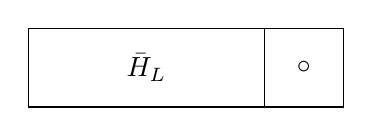
\begin{tikzpicture}
      \draw (0,.5) rectangle (3,-.5) node [midway] {$\bar H_L$};
      \draw (3,.5) rectangle (4,-.5) node [midway] {\ensuremath\circ};
    \end{tikzpicture}}_{H_{L+1}}
  \]
\end{enumerate}

\subsection{Eigenstates of the $\psi_i = 1$, $m$, $L$-site system}

S. White: Enlarge the system first, and add the boundary condition to the
enlarged system, which has less effect to the original system.
Then, project to the original system.
For non-interaction, the effect is pretty good.

But for the system with interaction, the result of the projection is
\[
  \ket|\Psi_{Sb}> 
  \begin{aligned}
    & \to \ket|\Psi_L^{(1)}>\\
    & \to \ket|\Psi_L^{(2)}>\\
  \end{aligned}, \qq{multiple numbers}
\]
and $\ket|\Psi_L^{(-)}>$ is the most proper one.
When executing the caclculation,
\[
  \underbrace{
  \underbrace{
  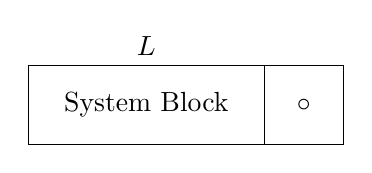
\begin{tikzpicture}
    \draw (0,.5) rectangle (3,-.5) node [midway] {System Block}
                 node [midway, above = .5cm] {$L$};
    \draw (3,.5) rectangle (4,-.5) node [midway] {\ensuremath\circ};
  \end{tikzpicture}}_{\text{$L+1$ System superblock}}
  \quad
  \underbrace{
  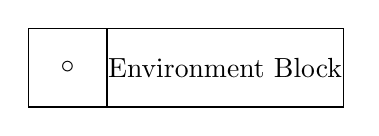
\begin{tikzpicture}
    \draw (0,.5) rectangle (3,-.5) node [midway] {Environment Block};
    \draw (-1,.5) rectangle (0,-.5) node [midway] {\ensuremath\circ};
  \end{tikzpicture}}_{\text{Environment superblock}}}_{\text{Superblock OBC}}
\]
\begin{enumext}
  \item Construct a basic state number and a superblock which needs exceed $m$
  but also small enough for exact diagonalization.
  \item Exactly diagnose the superblock, and take the lowest eigenstate ($m$)
  \item These states use system Sb basic state $\ket|i>$ and $CSb\ket|j>$
  \[
    \ket|\psi> = \sum_{ij} \psi_{ij} \ket|i>\ket|j>
  \]
  then project to the reduced density matrix of the sysbem Sb
  \[
    \rho_{ii'} = \sum_{j \text{(environment)}} \ketbra|\psi><\psi|
  \]
  where $\Tr\rho = 1$, then we can diagonalize $\rho$, the eigenvalues $W_\alpha \geq 0$, and $\sum_\alpha w_\alpha = 1$, and the eigenstates
  $\ket|u^\alpha>$.
  \item If $\alpha = 1$, $\ldots\,$,~$s$, then
  \begin{enumext}
    \item If $s \leq m$, then keep all the states;
    \item If $s > m$, them keep the $n$ maximum states of $w^\alpha$ in the $s$
    states.
  \end{enumext}
\end{enumext}

\begin{example}
  1D spin $\sfrac12$ AFM Heisenberg model
  \[
    H = \sum_i \bm S_i \bm S_{i+1}, \qq{let}
    m = S, S^z_\text{tot} = 0
  \]
  the so-called antiferromagnetic model.
  \begin{enumext}
    \item $L = 4$, the Superblock
    \[
      \underbrace{\underset{\text{Sys}}{\square}--
      \circ}_{\text{Sys Sb}}--\underbrace{\circ--
      \underset{\text{Cir}}{\square}}_{\text{Cir Sb}}
    \]
    contains $B_L$, $S_L$, $S_R$, $B_R$ respectively in the figure, and
    \begin{align*}
      & H_{B_L} = H_{S_L} = H_{S_R} = H_{B_R} = 0\\
      & S_{B_L}^z = S_{S_L}^z = S_{S_R}^z = S_{B_L}^z =
      \pdiagmat*{\sfrac12,\sfrac12}\\
      & S_{B_L}^+ = S_{S_L}^+ = S_{S_R}^+ = S_{B_L}^+ =
      \begin{psmallmatrix}
        0 & 1\\0 & 0
      \end{psmallmatrix}\\
      & S_{B_L}^- = \cdots =
      \begin{psmallmatrix}
        0 & 0\\1 & 0
      \end{psmallmatrix}
    \end{align*}
    The 4 blocks, to keep $S_\text{tot}^z = 0$, there are 6 states
    \[
      \ab(
        \begin{aligned}
        & \ket*|\frac12, \frac12, -\frac12, -\frac12>\\
        & \ket*|\frac12, -\frac12, \frac12, -\frac12>\\
        & \ket*|\frac12, -\frac12, -\frac12, \frac12>\\
        & \ket*|-\frac12, \frac12, \frac12, -\frac12>\\
        & \ket*|-\frac12, \frac12, -\frac12, \frac12>\\
        & \ket*|-\frac12, -\frac12, \frac12, \frac12>
        \end{aligned}
      )
    \]
    then, the Hamiltonian
    \[
      \hat H = \bm S_{B_L} \cdot \bm S_{S_L} + \bm S_{S_L} \cdot \bm S_{S_R}
            + \bm S_{S_R} \cdot \bm S_{B_R} =
      \begin{pmatrix}
        \frac14 & \frac12 & 0 & 0 & 0 & 0\\
        \frac12 & -\frac34 & \frac12 & \frac12 & 0 & 0\\
        0 & \frac12 & -\frac14 & 0 & \frac12 & 0\\
        0 & \frac12 & 0 & -\frac14 & \frac12 & 0\\
        0 & 0 & \frac12 & \frac12 & -\frac14 & \frac12\\
        0 & 0 & 0 & 0 & \frac12 & \frac12
      \end{pmatrix}
    \]
    The eigenvector
    \[
      \ket|\psi> =
      (0.149429, -0.557678, 0.408248, -0.557678, -.149427)\tran
    = \psi_{\frac12\frac12-\frac12\frac12-\frac12-\frac12} + \cdots
    \]
    and the density matrix element
    \[
      \rho_{i_1,i_2,i_1',i_2'}
    = \sum_{j_1j_2} \psi_{i_1i_2j_1j_2} \psi_{j_1j_2i_1'i_2'}
    \]
    from the basis
    \[
      \{\ket|i_1, i_2>\} =
      \{
        (\sfrac12,\sfrac12),
        (\sfrac12,-\sfrac12),
        (-\sfrac12,\sfrac12),
        (-\sfrac12,-\sfrac12)
      \}
    \]
    the density matrix is
    \[
      \rho = \begin{pmatrix}
        -0.022329 & 0 & 0 & 0\\
        0 & -0.477671 & 0.455342 & 0\\
        0 & 0.455342 & -0.477671 & 0\\
        0 & 0 & 0 & -0.022329
      \end{pmatrix}.
    \]
    Diagonalize $\rho$
    \[
      W = (0.022329, 0.933013, 0.022329, 0.022329)
    \]
    \[
      u^1 = (1,0,0,0)\tran,
      u^2 = (0,\sfrac{\sqrt2}{2},-\sfrac{\sqrt2}{2},0)\tran,
      u^3 = (0,\sfrac{\sqrt2}{2},\sfrac{\sqrt2}{2},0)\tran,
      u^4 = (0,0,0,1)\tran
    \]
    $S = 4\times 5$ matrix.
    \item $L = 2$.
  \end{enumext}
\end{example}

\section{K-T Phase Transition}

The spin on a 2D plane
\begin{equation}
  \bm S = (S_x, S_y), \qq{and}
  \mathcal H = -J'\sum_{\braket<ij>} \bm S_i \cdot \bm S_j
             = -\underbrace{J'S^2}_J \sum_{\braket<ij>}
              \cos(\theta_i - \theta_j)
\end{equation}
i.e., $X-Y$ model.
\begin{center}
  \begin{minipage}{.48\linewidth}
    \centering
    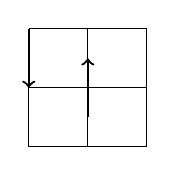
\begin{tikzpicture}[scale = .75]
      \draw (0,0) grid (2,2);
      \draw [thick, ->] (1,.5) --++ (0,1);
      \draw [thick, ->] (0,2) --++ (0,-1);
    \end{tikzpicture}
  \end{minipage}
  \hspace*\fill
  \begin{minipage}{.48\linewidth}
    \centering
    \begin{tikzpicture}
      \draw (0,0) -- (3.5,0);
      \draw [->, thick] (0,0) node [below] {$i$} --++ (1,.5)
       node [above] {$\bm S_i$};
      \draw [->, thick] (2,0) node [below] {$j$} --++ (.5,1)
       node [above] {$\bm S_j$};
    \end{tikzpicture}
  \end{minipage}
\end{center}
The partition function
\begin{equation}
  Z = \Tr \upe^{-\beta H} = \int_0^{2\pi} \prod_i \frac{\d\theta_i}{2\pi}
      \upe^{-\beta H(\theta_i)}
  \xlongequal{T \gg J/k_B}
    \int_0^{2\pi} \prod \frac{\d\theta_i}{2\pi} \prod_{\braket<ij>}
    (1 + \beta J\cos(\theta_i - \theta_j) + \mathcal O(\beta J)^2)
\end{equation}
Therefore
\begin{equation}
  \begin{aligned}
    \braket<\bm S_0 \cdot \bm S_1> & = S^2 \int_0^{2\pi}
    \prod_i \frac{\d\theta}{2\pi} \prod_{\braket<ij>}
    (1 + \beta J\cos(\theta_i - \theta_j))
    \cos(\theta_0 - \theta_i) \sim \ab(\frac{\beta J}{2})^{|\bm r|}\\
    & = \exp\ab(-\ln|\ab(\frac2{\beta J})^{|\bm r|}|)
    \equiv \exp\ab(-\frac{|\bm r|}{\xi})
  \end{aligned}
\end{equation}
where $\xi^{-1} = \ln\frac2{\beta J}$. The exponential state stands for the
disorder. This is so-called the \emph{High-temperature expansion.}

For \emph{Low-temperature expansion}, $\beta J \geq 1$.
It should near a ferronmagnetic state, so
$\theta_i - \theta_j \ll 1$,
$\cos(\theta_i - \theta_j) = 1 - \frac12(\theta_i - \theta_j)^2$.
\[
  (\theta_i - \theta_{i+\delta x})^2 + (\theta_i - \theta_{i+\delta y})^2
\Rightarrow a^2(\pdif x\theta_i)^2 + a^2(\pdif y\theta_i)^2
= a^2(\nabla \theta_i)^2
\]
At the continuous limit
\[
  \beta H = \beta E_0 - \frac{\beta J}{2} |\nabla\theta(x)|^2
\]
where $\beta E_0 = 2\beta JL^2/a^2$, $\braket<\cos(\theta_0-\theta_1)>
\sim |\bm r/a|^{-1/(2\pi\beta J)}$.
It is power low decay, we call it \emph{Quasi-long order}, or \emph{algebric},
or \emph{long range order}.

Take a peek $\fdv H\theta = 0$, then,
\[
  -(\nabla\theta)^2 = \theta\nabla^2\theta - \nabla(\theta\nabla\theta)
\]
we have $\nabla^2\theta = 0$.
\begin{enumext}
  \item $\theta = \text{Const}$
  \item $\nabla\theta = \ab(-\frac g{r^2}, \frac x{r^2})$,
        $\theta = \arctan(\frac yx)$, which satisfies
        $\oint \nabla\theta \d\bm r = 2\pi$
  \item Common solution: $\oint \nabla \theta \d\bm l = 2\pi n$
  
  The Hamiltonian
  \[
    H = -\theta \nabla^2\theta \to (\nabla\theta)^2
  \]
  where
  \[
    \nabla \theta \cdot \nabla\theta = \frac{x^2 + y^2}{r^4} = \frac1{r^2}
  \]
  Then, the integral
  \[
    \frac J2 \int \d^2 \bm r (\nabla\theta)^2 - E_0
  = \frac J2 \int_a^L r \d r \int_0^{2\pi} \d\theta \frac1{r^2}
  = J\pi \ln \frac La
  \]
  This kind of solution is a high-energy excitation at $T = 0$.

  Consider a pair of vertices: $\theta_1 - \theta_2 \approxeq 0$,
  $|\bm r_{12} \to \infty|$ with finite energy.
  \begin{center}
    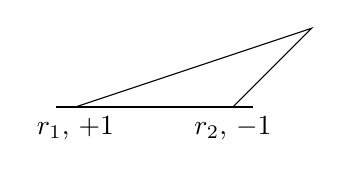
\begin{tikzpicture}
      \draw (-1.25,0) -- (1.25,0);
      \draw (-1,0) node [below] {$\bm r_1$, $+1$} -- (2,1) -- (1,0)
       node [below] {$\bm r_2$, $-1$};
    \end{tikzpicture}
  \end{center}
  \begin{align*}
    E_\text{vortex-pair} &
  = \int \d^2\bm r[(\nabla\theta_1)^2 + (\nabla\theta_2)^2]
  \approxeq \int_\text{core} \d^2\bm r(\nabla\theta_1)^2
            \int_\text{core} \d^2\bm r(\nabla\theta_2)^2\\
& = \int_a^R r \d r (\nabla\theta_1)^2 \d\theta +
    \int_a^R r\d r \d\theta (\nabla\theta_2)^2
  = 2E_\text{core} + 2J\pi\ln\frac Ra
  \end{align*}
  The 2D Column gas
  \[
    F = -\pdv ER = -\frac1R
  \]
  At a finite temperature, a vortex's square proportion to $a^2$.
  In a square of $L^2$, there can be around $L^2/a^2$ positions of vortices.
  The entropy
  \[
    S = \ln \ab(\frac{L^2}{a^2})
  \]
  then, the free energy of a vortex is
  \[
    F = U - TS = (J\pi\ln\frac La - T\ln\ab(\frac{L^2}{a^2}))
      = (J\pi - \frac2\beta) \ln\frac La
  \]
  If $J\pi - 2/\beta < 0$, then a single vortex can escape from the vortex-pair;
  and take a phase transition to becomes favorable.
  The critical temperature $T_c = J\pi/2k_B$.
\end{enumext}
\chapter{Non-equilibirum Statistic Physics}

\section{Boltzmann integral ODE}

At the equilibirum state, we have a distribution function, aka a function of the energy that independent from the time
\begin{equation}
  f_0 = f_0(\bm r) = f_0(E)
\end{equation}
which only depends on $r$ and $E$.
\begin{equation}
  f_0 = \frac1{\upe^{\beta E} \pm 1} \xrightarrow{Non-equilibirum}
  f(\bm r, \bm v, t)
\end{equation}
This is the Boltzmann equation for the classical short-term interaction thin gas.
\begin{enumext}
  \item Classical: $\lambda_T \ll |\overline{\delta r}|$,
  $\lambda_T = \frac h{(2\pi mk_BT)^{1/2}}$ is the high-temperature wavelength.
  The gas under the standard state
  ($\qty0\degreeCelsius$, $\qty1{atm}$).
  For the Argon: $n = \qty{2.7e19}{\cm^{-3}}$, $m \approx \qty{6.7e-23}\g$.
  Then
  \[
    \lambda_T = \frac{h}{\sqrt{2\pi mk_BT}} \sim \qty{0.17e-8}\cm, \qq{and}
    \frac{\overline{\delta r}}{\lambda_T} \approxeq 190.
  \]
  \item Thin and Short-term force $\overline{\delta r} \gg d$.
  Most of the gas molecules are free most time.
  Separate the ``hit'' and the ``motion'':
  There is no motion when hitting, or there will be no hitting when moving.
  \[
    \overline{\delta r} \approxeq \qty{3.3e-7}\cm, \quad
    m \sim \qty{6.7e-23}\g, \quad
    \lambda_T = \frac{h}{\sqrt{2\pi mk_BT}} \approxeq \qty{0.17e-8}\cm
  \]
  \item Three-body hitting can be omitted
  
  Taking another simplification
  \begin{enumext}
    \item Omit the structure of molecules, take the rigid-sphere model to instead the Van der Waals force.
    \item There's no relation between the velocities of two hitting molecules.
  \end{enumext}
\end{enumext}
To derive the evolution of $f(\bm r, \bm v, t)$
\[
  f(\bm r, \bm v, t) \d^3\bm r \d^3 \bm v
\]
is the average number of moleculese around the volume unit in the phase
($\bm r$, $\bm v$).
From $t \to t + \d t$
\[
  \frac1{\d t} [f(\bm r, \bm v, t + \d t) - f(\bm r, \bm v, t + \d t)]
  \d^3\bm r \d^3\bm v = \pdv ft \d^3\bm r \d^3\bm v
\]
where $\pdv ft = \ab(\pdv ft)_d + \ab(\pdv ft)_c$: d stands for the drift,
and c stands for the collision.

\subsection{Derivation of the drift term}

Since
\[
  \d f = \ab[f(\bm r + \dot{\bm r} \d t, \bm v + d\bm v, t + \d t)
            -f(\bm r, \bm v, t)] \d t = 0
\]
then,
\[
  \odv ft = \ab(\pdv ft)_d + \sum_i \ab(\dot x_i \pdv f{\dot x_i}
+ \dot v_i \pdv f{v_i}) = 0
\]
So, the drift term
\[
  \ab(\pdv ft)_d = -\bm r \cdot \pdv fr - \bm r \cdot \pdv f{\bm r}
= -\pdv*{\bm rf}{\bm r} - \pdv*{\bm vf}{\bm v}
\]

\subsection{Derivation of the collision term}

To derive the collision term, consider the collision between two particles
\begin{gather*}
  m_1 \bm v_1 + m_2 \bm v_2 = m_1 \bm v_1' + m_2 \bm v_2'\\
  \frac12m_1 v_1^2 + \frac12m_2 v_2^2 = 
  \frac12m_1 v_1'^2 + \frac12m_2 v_2'^2
\end{gather*}
Since at the normal dirction, $v_{1_\bot}' = v_{1_\bot}$.
Then the bound condition
\[
  \bm v_1' - \bm v_1 = \lambda_1 \bm n, \qq{and}
  \bm v_2' - \bm v_2 = \lambda_2 \bm n
\]
For a given $\bm n$, we can solve
\begin{gather*}
  \bm v_1' = \bm v_1 + \frac{2m_2}{m_1 + m_2} [(\bm v_2 - \bm v_1) \cdot \bm n] \bm n\\
  \bm v_2' = \bm v_12 - \frac{2m_1}{m_1 + m_2} [(\bm v_2 - \bm v_1) \cdot \bm n] \bm n
\end{gather*}
Then, we have
\[
  \bm v_2' - \bm v_1' = \bm v_2 - \bm v_1' - 2[(\bm v_2 - \bm v_1) \cdot \bm n] \bm n, \quad
  (\bm v_2' - \bm v_1')^2 = (\bm v_2 - \bm v_1)^2, \quad
  v_{12}'^2 = v_{12}^2.
\]
To calculate $\ab(\pdv ft)_c$
\[
  f_i = f(\bm r, \bm v_i, t), \quad f_i'(\bm r, \bm v_i', t)
\]
$\Delta f_1^{(t)}$ is the collision in the $\d^3\bm r$ space during the $\d t$ time. Then,
\[
  \ab(\pdv{f_1}t)_c \d t \d^3\bm r \d^3\bm r_1
= \Delta f_1^{(+)} - \Delta f_1^{(-)}
\]
When the two molecules collide, if collide with the $m_2$ molecule with the
centre of $\bm r_2$ within the volume unit of $\d^3\bm r_2$, then, the collision
direction will be limited in the cubic angle $\d\Omega$ with the normal vector $\bm n$.

Then, it must be limited in a cylinder with height $v_{12} \cos\theta\d t$ and
with the lower square $r_{12}^2\d\Omega$.
The volume of the cylinder is $r_{12}^2 \d\Omega v_{12} \cos\theta\d t$,
where includes the number of molecules with $\d^3v_{12}$
\[
  (f_2\d^3r_2) r_{12}I^2 \d\Omega v_{12} \cos\theta \d t
\]
Multiply the number of molecules $m$
\[
  (f_1 \d^3\bm r \d^3\bm v_1)(f_2 \d^3r_2) r_{12} \d\Omega v_{12}\cos\theta \d t
\]
equal to the number of collisions between molecules in $\d^3\bm r \d^3\bm v_1$
and molecules in $\d^3\bm r_2$ within the $\d\Omega$ direction during time
$\d t$ is equal to the number of collisions between molecules in
$\d^3\bm r \d^3\bm v_1$ and molecules in $\d^3\bm r_2$ within the domega
direction.

$\delta f_1^{(-)}$ enable the decrease of molecules within $\d^3\bm v_1$:
$(\bm v_1, \bm v_2) \to (\bm v_1', \bm v_2')$
\[
  \delta f_1^{(+)} = \ab[f_1' f_2' \lambda_{12}' \d\Omega' \d^3\bm v_2']
  \d t \d^3\bm r_1 \d^3 \bm v_1'
\]
with $(\bm v_1', \bm v_2', -\bm n) \to (\bm v_1, \bm v_2)$, and the transformation
\[
  \d^3 \bm v_1' \d^3\bm v_2' = \d^3v_1 \d^3\bm v_2
  \begin{vmatrix}
    \pdv{v_1}{v_1'} & \pdv{v_2}{v_1'}\\
    \pdv{v_1}{v_2'} & \pdv{v_2}{v_2'}
  \end{vmatrix}.
\]
Then,
\[
  \ab(\pdv ft)_c \d t \d^3\bm r_1 \d^3\bm v_1 = \Delta f_1^{(+)} - \Delta f_1^{(-)}
  = \int [(f_1'f_2' - f_1f_2) \d^3\bm v_2 \lambda_{12} \d\Omega] \d t \d^3\bm v_1 \d^3\bm v_1
\]
\[
  \pdv ft - \ab(\pdv ft)_d = \ab(\pdv ft)_c
\]
\[
  \pdv ft + \bm v \cdot \ab(\pdv fr) + \bm g \cdot \pdv f{\bm v}
= \int(f_v' f_w' - f_vf_w)  \lambda \d^3 \bm\omega \d\Omega
\]

\section{$H$-theomre, $H$-function and entropy}

The Entropy
\begin{equation}
  S = -\sum_i p_i \ln p_i
\end{equation}
The $H$-function
\begin{equation}
  H = \int f(\bm r, \bm v, t) \ln f(\bm r, \bm v, t) \d^3\bm v \d^3\bm r
\end{equation}
The gas at the equilibirum state
\[
  n = N/V
\]
The Maxwell distribution
\begin{equation}
  f = n\ab(\frac m{2\pi k_BT})^{3/2} \exp\ab(-\frac{mv^2}{2k_BT})
\end{equation}
Then, the $H$-function becomes
\begin{equation}
  H = \int f\ab[\ln n + \frac32\ln\frac m{2\pi k_BT} - \frac{mv^2}{2k_BT}]
      \d^3\bm r \d^3\bm v
\end{equation}
where the integral
\[
  \int f \d^3\bm r \d^3\bm v = n, \quad
  \frac1n\int\frac{mv^2}{2} f\d^3\bm v = \frac32k_BT
\]
The entropy of single-atom ideal gas
\[
  S = Nk_B\ab[\ln\frac VN + \frac32\ln T + \frac52 + \frac32\ln\ab(\frac{2\pi mk_B}{h^2})]
= -k_BH + C
\]
Use the Boltzmann equation to derive the $H$-theorem
\begin{equation}
  \odv HT \leq 0
\end{equation}
The time derivative to $H$
\begin{align*}
  \odv HT & = \int \ab(\pdv ft \ln F + f \cdot \frac1f) \d^3\bm r \d^3\bm v
  = \int (1 + \ln f) \pdv ft \d^3\bm r \d^3\bm v\\
& = -\int (1 + \ln f) \ab(\bm v \cdot \pdv f{\bm r}) \d^3\bm r \d^3\bm v
  -\int (1 + \ln f)(\bm q \cdot \pdv f{\bm v}) \d^3\bm r \d^3\bm v
  -\int (1 + \ln f)(f_1f_2 - f_1'f_2') \d^3\bm v\d^3\bm v'
    \Lambda \d\Omega \d^3\bm r
\end{align*}
The first term
\[
  \nabla \cdot(\bm v f\ln f) = \bm v(1 + \ln f) \pdv f{\bm r}
\]
\[
  \int \d^3\bm r \nabla \cdot (\bm v f \ln f)
= \oiint \bm n \cdot (\bm v f - \ln f) \d\Sigma = 0
\]
The second term $\pdv*{\bm q}{\bm v} = 0$
\[
  \int\pdv*{\bm q f\ln f}{\bm v} \d^3\bm v
= \oiint \d\bm S_v \cdot \bm q f \ln f
\]
when $v \to \infty$, $ f(v)\big|_{v\to\infty} = 0$.
The third term: $1 \leftrightarrow 2$,
\[
  \odv HT = -\int (1 + \ln f_2)(f_1f_2 - f_1'f_2') \d^3\bm v_1 \d^3\bm r_2
  \Lambda \d\omega \d^3\bm r
\]
Combine and then half
\[
  \odv Ht = -\frac12 \int (2 + \ln(f_1f_2)) (f_1f_2 - f_1'f_2') \d(\cdots)
\]
$v_{1,2}' \leftrightarrow v_{1,2}$, we have
\[
  \odv Ht = -\frac12 \int (2 + \ln (f_2'f_1;)) (f_1'f_2' - f_1f_2) \d(\cdots)
= -\frac14 \underbrace{
    \ab(\ln(f_1f_2) - \ln(f_1'f_2^2)) (f_1f_1 - f_1'f_2') \d(\cdots)}_{\geq 0}
\]
Then, $\odv Ht \leq 0$, $\odv St \geq 0$.
When $f_1f_2 = f_1'f_2'$ (Detailed equilibrium condition), they equal to zero.

\section{Application of Boltzmann Equation}

The relaxation time approximation
\begin{equation}
  \ab(\pdv ft)_c = -\frac{f - f^{(0)}}{\tau}
\end{equation}
where $\tau$ is the relaxation time that tends to equilibirum, independent of
$\bm r$. Assum $f$ is also independent of $\bm r$.
Without the external force,
\[
  \pdv ft = -\frac{f - f^{(0)}}{t}
\]
Then, we have
\begin{gather*}
  \frac{\d(f - f^{(0)})}{f - f^{(0)}} = -\frac{\d t}{\tau},\\
  f(\bm v) - f^{(0)}(\bm v) = [f(\bm v, 0) - f^{(0)}(\bm v)] \upe^{-t/\tau}
\end{gather*}
$\tau$ is the time that required by tending to equilibirum.
In the free electon gas,
\[
  f^{(0)}(\bm p) = \frac1{\upe^{(\epsilon(p) - \mu)/k_BT} + 1}
\]
and the Fermi energy $\epsilon(p) = \frac{p^2}{2m}$.

In the unit volume, the average electron number that with in the momentum range
$\d^3\bm p$ is $2\frac{\d^3\bm p}{h^3} f^{(0)}$.

The Boltzmann equation
\[
  \pdv ft + \frac{\bm p}{m} \cdot \pdv f{\bm r} + \bm F \cdot \pdv f{\bm p}
= -\frac{f - f^{(0)}}{\tau}
\]
where $\bm F = -e\bm E$, i.e., the ecurrent is a uniform and eternal
\[
  \pdv ft = 0, \quad \nabla f = 0, -e\bm E \cdot \pdv f{\bm p} = -\frac{f - f^{(0)}}{\tau}
\]
where $f = f^{(0)} + f^{(1) + \cdots}$, and we keep the first order
\[
  e\bm E \cdot \pdv{f^{(0)}}{\bm p} = \frac{f^{(1)}}{\tau} \quad
  f^{(1)} = e\tau\bm E \cdot \bm v \pdv{f^{(0)}}E
\]
Hence,
\[
  f \approxeq f^{(0)} + e\tau \bm E \cdot \bm v \pdv{f^{(0)}}\epsilon
  = f^{(0)}(\epsilon + e\tau\bm E \cdot \bm v)
\]
where
\[
  \pdv{f^{(0)}}{\bm p} = \pdv{f^{(0)}}\epsilon  \pdv\epsilon\beta
= \pdv{f^{(0)}}\epsilon \bm v
\]
The $\bm E$ patt through $\d\bm A$ perpendicularly, hence
\[
  \int J_e \d t \d A = e\int v_x \d t \d A f\frac{2\d^3\bm p}{h^3}
\]
where
\[
  J_e = nev_x = \frac{2\d^3\bm p}{h^3} f ev_x
= 2e\int v_x(\cancel{f^{(0)}} + f^{(1)}) \frac{\d^3\bm p}{h^3}
\]
and we have
\[
  v_p = \frac km, \qq{and} f^{(0)}(v_x) = f^{(0)}(-v_x)
\]
Now, handel $\d^3\bm p$
\[
  \d^3\bm p = p^2\d p \int \d\theta \sin\theta\d\varphi
= 2m\epsilon \d(\sqrt{2m}\sqrt\epsilon) \cdot 4\pi
= \frac{4\pi(2m)^{3/2}}{2} \epsilon^{1/2} \d\epsilon
\]
Substitute it into $J_e$
\[
  J_e = 2eEt \int v_x^2 \pdv{f^{(0)}}\epsilon \frac{\d^3\bm p}{h^3}
= e^2 E\tau, \quad
  \int v_x^2 \pdv{f^{(0)}}\epsilon D(\epsilon) \d\epsilon
\]
where
\[
  D(\epsilon) = 4\pi \frac{(2m)^{3/2}}{h^3} \epsilon^{1/2}
\]
Finally,
\[
  J_e = e^2E\int \tau \frac{v^3}{3} \pdv{f^{(0)}}t D(\epsilon) \d\epsilon
\]
Around $T \sim 0$, $f^{(0)} = \theta(\epsilon - \mu)$. Then,
\[
  J = \frac{2e^2t}{3m} \mu D(\mu) E, \quad
  n = \int_0^\mu D(\epsilon) \d\epsilon = \frac23 \mu D(\mu)
\]
We can use it to calculate the conductivity,
\[
  J_e = \frac{ne^2\tau}{m} E = \sigma E, \qq{where} \sigma = \frac{ne\tau}{m}
\]
The force
\begin{equation}
  \bm F = -e\bm E - \frac ec \bm v \times \bm B
\end{equation}
where $\bm v = (v_x, v_y)$, $v = v_x + \iu v_y$.
The stability
\[
  \pdv ft + \bm v \cdot \nabla f = 0
= -\frac{\bm F}{m} \cdot \pdv f{\bm v} + \ab(\pdv ft)_c
\]
The derivative
\[
  0 = \odv{\braket<v>}t
    = -\frac{eE}{m} + \iu\omega_c \braket<v> - \frac{\braket<v>}{\tau},
  \qq{where}
  \braket<v> = -\frac{eE/m}{1 - \iu\omega_c\tau}
\]
Substitute $E = E_x + \iu E_y$, $\omega_c = \frac{eB}{mc}$,
the current density
\[
  \bm j = \mathbf \sigma \cdot \bm E =
  \begin{pmatrix}
    \sigma_{xx} & \sigma_{xy}\\
    \sigma_{yx} & \sigma_{yy}
  \end{pmatrix}
  \begin{pmatrix}
    E_x \\ E_y
  \end{pmatrix} = j_x + \iu j_y
\]
So, we have the elements of the conductivity matrix
\[
  \sigma_{xx} = \sigma_{yy} = \frac{\sigma_0}{1 + \omega^2\tau^2}, \quad
  \sigma_{xy} = -\sigma_{yx} = -\frac{nce}{B} - \frac{\sigma_{xx}}{\omega_c\tau}
\]
where $\sigma_0 = \frac{ne^2\tau}{m}$.

\section{Fluctuation Phenomenon: Themoral Variables}

\subsection{Regrex System}

The fluctuation of energy
\begin{equation}
  \frac{\sqrt{\braket<(E - \braket<E>)^2>}}{\braket<E>} \sim \frac1{\sqrt N},
  \qq{and} n = \frac NV \qq{finite}
\end{equation}
are all the fluctuations corresponding the microscope variable.

\subsection{Quasi-Themoral Theory (Smoluchowski-Einstein Method)}


The theromal entropy
\begin{equation}
  \bar S = k_B \ln W_{\max} \qq{(theromal probability)}
\end{equation}
where $W_{\max} = \upe^{\bar S/k_B}$.

The differ from equilibirum
\[
  W = \upe^{S/k_B} = W_{\max} \upe^{(S - \bar S)/k_B}
    = W_{\max} \upe^{\Delta S/k_B}
\]
\begin{enumext}
  \item For dependent system, $\Delta E = 0$, $\Delta V = 0$.
  \item For regrex system,
  $\Delta E + \Delta E_e = 0$,
  $\Delta V + \Delta V_e = 0$.
  \begin{align*}
    W_T & = W_{\max} \upe^{(\Delta S + \Delta S_e)/k_B}
  = W_{\max} \upe^{\ab(\Delta S + \frac{\Delta E_e + pV_e}{T})/k_B}\\ &
  = W_{\max} \upe^{(\Delta S T - \Delta E - p\Delta V)/(k_BT)}
  = W_{\max} \upe^{-(\Delta F + p\Delta V)/(k_BT)}
  \end{align*}
\end{enumext}
The free energy
\begin{equation}
  \Delta F = \underbrace{\ab(\pdv FV)_T}_{-p} \delta V
  + \frac12 \underbrace{\ab(\pdv[2]FV)_T}_{-\pdv p/V} (\Delta V)^2
  + \cdots
\end{equation}
Then,
\begin{equation}
  W_T \approxeq W_{\max} \exp\ab[\frac1{2k_BT} \ab(\pdv pV)_T (\Delta V)^2]
\end{equation}
The probability of the quasi-themoral in regrex system
\begin{equation}
  \braket<(\Delta A)^2>
= \frac{\int (\Delta A^2) W \d(\Delta A)}{\int W\d(\Delta A)}
\end{equation}
\begin{example}
  Calculate $\braket<(\Delta V)^2>$.
  \begin{align*}
  & \frac{\int_{-\infty}^\infty (\Delta V)^2
      \exp\ab[\frac1{2k_BT}\ab(\pdv PV)_T(\Delta V)^2] \d(\Delta V)}
    {\text{normalization factor}}\\
= & \frac1{\int \cdots} \int_{-\infty}^\infty (\Delta V)^2
    \frac{k_BT}{(\pdv p/V)_T}
    \frac1{\Delta V} \d\ab\{\exp\ab[\frac1{2k_BT} (\pdv p/V)_T (\Delta V)^2]\}\\
= & \frac1{\int \cdots} \frac{\Delta V(k_BT)}{(\pdv p/V)_T}
    \exp\ab[-\frac1{2k_BT}\ab|\ab(\pdv pV)_T| (\Delta V)^2]
    \bigg|_{-\infty}^\infty - k_BT \ab(\pdv Vp)_T = -k_BT\ab(\pdv Vp)_T
  \end{align*}
  Then, we have
  \[
    \frac{\braket<(\Delta V)^2>}{V^2} = -\frac{k_BT}{V^2} \ab(\pdv Vp)_T
  \]
  If the mass of the system $M = \text{Const}$, i.e., $M = pV$ is fixed. Then,
  \[
    \Delta M = \Delta\rho V + \rho\Delta V = 0 \Rightarrow
    \frac{\Delta\rho}{\rho} = -\frac{\Delta V}{V}, \quad
    \frac{\braket<(\Delta\rho)^2>}{\rho^2} = \frac{\braket<(\Delta V)^2>}{V^2}
  = -k_BT \ab(\pdv Vp)
  \]
  $\rho = N/V$, if $V$ is fixed, then $\Delta \rho \propto \Delta N$.
  \begin{gather*}
    \braket*<\ab(\frac{\Delta N}{N})^2> =
    \braket*<\ab(\frac{\Delta \rho}{\rho})^2> = -\frac{k_BT}{V^2} \ab(\pdv Vp)_T\\
    \Delta\rho = \frac{\Delta N}{V} - \frac{N\Delta V}{V^2}\\
    (\Delta\rho)^2 = \ab(\frac{\Delta N}{V})^2 - \frac{2\Delta N\Delta V}{V^3} + \frac{N^2(\Delta V)^2}{V^4}\\
    \braket<(\Delta \rho)^2> = \braket<\ab(\frac{\Delta N}{V})^2> + \frac{N^2\braket<(\Delta V)^2>}{V^4}\\
    \frac{\braket<(\Delta\rho)^2>}{N^2} =
    \frac{\braket<(\Delta N)^2>}{N^2} + \frac{\braket<(\Delta N)^2>}{N^2}
  = 2\braket<\ab(\frac{\Delta N}{N})^2>
  \end{gather*}
  The critical point
  \[
    \ab(\pdv pV)_T = \ab(\pdv[2]pV)_T = 0
  \]
  Then,
  \[
    \Delta F = -p\Delta V - \frac1{4!} \ab(\pdv[3]pV)_T (\Delta V)^4 + \cdots
  \]
  \[
    W = W_{\max} \exp(-\alpha x^4), \quad x = \Delta V
  \]
  \[
    \braket<(\Delta V)^2>
  = \frac{\int_0^\infty x^2 \upe^{-\alpha x^4} \d x}
      {\int_0^\infty \upe^{-\alpha x^4} \d x}
  = \frac{\Gamma(\frac34)}{\Gamma(\frac14)} \frac1{\sqrt\alpha}
  = 0.338\frac1{\sqrt\alpha}
  \]
\end{example}

\subsection{Vande vars Gas}

\[
  p_c = \frac a{27b^2}, \quad v_c = 3b, \quad T_c = \frac{8a}{27bR}
\]
Substitute them into the ideal gas formula
\[
  \ab(p + \frac a{v^2}) (v - b) = RT, \quad
  p = \frac{3RT}{3V - V_c} - \frac{9RT_cv_c}{8v^2}, \quad
  V = \frac N{N_a} \sigma, \quad N_a = \num{6.02e23}
\]
Then,
\[
  p = \frac{3Nk_BT}{3V - V_c} - \frac{9N k_BT_cV_c}{8V^2}
\]
The derivatives
\begin{gather*}
  \ab(\pdv[3]pV)_T = -\frac{486Nk_BT}{(3V - V_c)^4} + \frac{27Nk_BT_cV_c}{V^5}\\
  \ab(\pdv[3]pV)_{T_c} = -\frac{27Nk_BT_c}{8V_c^4}
\end{gather*}
Finally, we have
\[
  \ab(\frac{\Delta V}V)_c^2 = 0.338\ab[-\frac{V_c^4}{24kT_c} \ab(\pdv[3]pV)_c]^{-1/2}
= 0.901/\sqrt N
\]

\begin{example}[The sky is blue (When the air is clean, not frog / haze)]
  The magnitude of the scatter of light
  \[
    I \propto \frac1{\lambda^4} \frac{\braket<(\Delta\rho)^2>}{\rho^2}
  \]
\end{example}

\begin{example}[Liquid]
  \[
    \frac{\braket<I>}{V} \propto
    \frac1{\lambda^4} V \ab[-\frac{V^4}{24k_BT}\ab(\pdv[3]pV)_T]^{1/2}
  \propto \frac1{\sqrt N}
  \]
\end{example}

\newcommand \sectionname {Lecture \#}
\appendix
\fancyhead[OL, ER]{Mingyu Xia (Westlake ID: 20251202247)}
\fancyhead[EL]{\sffamily \rightmark}
\fancyhead[OR]{\fontfamily{lmr}\selectfont<<\texttt{\href{mailto:xiamingyu@westlake.edu.cn}{xiamingyu@westlake.edu.cn}}>>}
\addcontentsline{toc}{chapter}{Problem Set}
\renewcommand *\thesection{\sectionname \arabic{section}}
\newweek
% !TeX root = ../main.tex

\section{Homework \#1 [2025-09-02]}

\begin{problem}
  总结热力学的基本概念:什么叫平衡态?写出温度、温标的定义;
  内能的定义;热容和比热的定义;熵的定义和物理意义.
\end{problem}
\begin{solution}\leavevmode
  \begin{enumext}
    \item 平衡态:在没有外界影响的条件下,
    物体各部分的性质长时间不发生任何变化的状态.
    \item 温度:衡量物体间是否热平衡的物理量称为温度.
    \item 温标:确定温度具体数值的规则叫温标.
    \item 内能:系统所含有的能量,但不包含因外部力场而产生的系统整体之动能与势能.
    \item 热容:在不发生相变化和化学变化的前提下,系统与环境所交换的热与由此引起的温度变化之比称为系统的热容.
    即 $C_\eta = \odv{Q_y}T$ 称为热容,其中 $\gamma$ 表示不变的量.
    \item 比热:单位质量的物质在温度变化时所吸收或释放的热量与其质量之比,即 $c = C/V$.
    \item 熵:一个系统内所有元素状态的总和,物理意义:用来衡量系统的无序程度.
  \end{enumext}
\end{solution}

\begin{problem}
  什么叫物态方程?写出理想气体的物态方程。写出范德瓦尔斯气体的物态方程,
  并解释对理想气体物态方程修正项的物理意义.
\end{problem}
\begin{solution}\leavevmode
  \begin{enumext}
    \item 物态方程:物体的物理状态由几何变量($V$, $A$, $L$),
    力学变量($p$, $\sigma$, $F$),电磁变量($\bm E$, $\bm P$, $\bm H$, $\bm M$)
    和化学变量等描述,温度与这些状态变量之间的函数关系
    $T = f(p, V, \cdots)$ 称为物态方程.
    \item 理想气体状态方程:$pV = nRT = NkT$
    \item 范德瓦尔斯气体的物态方程:$ab(p + \frac{n^2a}{V^2})(V - nb) = nRT$.
    \begin{enumext}
      \item 体积修正 $-nb$: 分子有固有体积,活动空间减少
      \item 压力修正 $+an^2/V^2$: 分子间吸引力减弱对器壁的冲击
    \end{enumext}
  \end{enumext}
\end{solution}

\begin{problem}
  对 $p-V-T$ 系统,依据自变量不同,写出 4 种等价的热力学微分方程,
  说明各自在什么条件下适用.
\end{problem}
\begin{solution}\leavevmode
  \begin{enumext}[columns = 2]
    \item $\d U = T\d S - p\d V ~ (S,V)$, 适用绝热过程
    \item $\d H = T\d S + V\d P ~ (S,P)$, 适用等压过程
    \item $\d F = -S\d T - p\d V$, 适用等温等容
    \item $\d G = -S\d T + V\d P$, 适用等温等压、相变
  \end{enumext}
\end{solution}

\pagebreak

\begin{problem}
  解释热力学第一、二、三定理的物理意义.
\end{problem}
\begin{solution}\leavevmode
  \begin{enumext}
    \item 热力学第一定律: 推广到非绝热过程,
    系统从外界吸热,$Q = U_2 - U_1 - W_0$,即能量守恒
    \item 热力学第二定律: 熵增加原理
    \item 热力学第三定律: 不可能通过有限步骤使物体冷却到绝对零度 
  \end{enumext}
\end{solution}

\begin{problem}[林宗涵《热力学与统计物理》 1.1]
  设三个函数 $f$, $g$, $h$ 都是二独立变量 $x$, $y$ 的函数,证明:
  \begin{enumext}[columns = 3]
    \item $\ab(\pdv fg)_h = 1/\ab(\pdv gf)_h$
    \item $\ab(\pdv fg)_x = \pdv fy/\pdv gy$
    \item $\ab(\pdv yx)_f = -\pdv fx/\pdv fy$
    \item $\ab(\pdv fg)_h \ab(\pdv gh)_f \ab(\pdv hf)_g = -1$
    \item $\ab(\pdv fx)_g = \pdv fx + \pdv fy\ab(\pdv yx)_g$
  \end{enumext}
\end{problem}
\begin{solution}\leavevmode
  \begin{enumext}
    \item 对 $f$ 取微分
    \[
      \d f = \ab(\pdv fg)_h \d g + \ab(\pdv fh)_g \d h
    \]
    令 $\d h = 0$ 得
    \[
      1 = \ab(\pdv fg)_h \ab(\pdv gf_h), \quad
      \ab(\pdv fg)_h = 1/\ab(\pdv gf)_h
    \]
    \item $f = f(x,y(x,g))$. 由复合函数求导法则
    \[
      \ab(\pdv fg)_x = \ab(\pdv fy)_x \ab(\pdv yg)_x
    = \ab(\pdv fy)_x \ab(\pdv gy)_x
    \]
    这里利用了 (a) 中的结论.
    \item $f = f(x,y)$. 令 $f$ 的微分为 $0$ 得
    \[
      \d f = \ab(\pdv fx)_y \d x + \ab(\pdv fy)_x \d y = 0,\quad
      \ab(\pdv yx)_f = -\ab(\pdv fx)_y/\ab(\pdv fy)_x
    \]
    \item $f = f(g,h)$. 对 (c) 中结论做变量替换
    \[
      \ab(\pdv hg)_f = -\ab(\pdv fg)_h/\ab(\pdv fh)_g
    \]
    利用 (a) 中的结论得
    \[
      \ab(\pdv fg)_h \ab(\pdv gh)_f \ab(\pdv hf)_g = -1
    \]
    \item $f = f(x,y(x,g))$. 由复合函数求导法则
    \[
      \ab(\pdv fx)_g = \ab(\pdv fx)_y + \ab(\pdv fy)_x \ab(\pdv yx)_g
    \]
  \end{enumext}
\end{solution}

\begin{problem}[林宗涵《热力学与统计物理》 1.5]
  有一铜块处于 $\qty0\degreeCelsius$ 和 $\qty1{atm}$ 下,
  经测定,其膨胀系数和等温压缩系数分别为 $\qty{4.85e-5}{\K^{-1}}$,
  $\kappa_\tau = \qty{7.8e-7}{(atm)^{-1}}$, $\alpha$ 和 $\kappa_\tau$
  可以近似当成常数. 今使铜块加热至 $\qty{10}\degreeCelsius$,问
  \begin{enumext}[columns = 2]
    \item 压强要增加多少才能维持铜块体积不变?
    \item 若压强增加 $\qty{100}{atm}$,铜块的体积改变多少?
  \end{enumext}
\end{problem}
\begin{solution}\leavevmode
  \begin{enumext}
    \item 在温度变化 $\d T$ 和压强变化 $\d p$ 范围内,铜块体积变化
    \[
      \d V = V(\alpha \d T - \kappa \d p)
    \]
    要维持铜块体积不变,则 $\d V = 0$,即
    \[
      \d p = \frac\alpha{\kappa_T}\d T = \qty{621.79}{atm}
    \]
    \item 对体积变化公式分离变量并积分得
    \[
      \ln \frac{V}{V_0} = \alpha \Delta T - \kappa_T \Delta p
    \]
    令 $V = V_0 + \Delta V$,则
    \[
      \ln\frac{V_0 + \Delta V}{V_0} \approx \frac{\Delta V}{V_0}
    = \alpha\Delta T - \kappa_T \Delta p = \num{4.07e-4}
    \]
    即铜块体积改变 $\qty{4.07e-2}\%$.
  \end{enumext}
\end{solution}

\begin{problem}[林宗涵《热力学与统计物理》 1.6]
  已知一理想弹性丝的物态方程为
  \[
    \mathcal F = bT\ab(\frac L{L_0} - \frac{L_0^2}{L^2})
  \]
  其中 $\mathcal F$ 使张力;$L$ 使长度,$L_0$ 使张力为零时的 $L$ 值,
  $L_0$ 只是温度 $T$ 的函数;$b$ 使常数. 定义(线)膨胀系数为
  \[
    \alpha \equiv \frac1L \ab(\pdv LT)_{\mathcal F}
  \]
  等温杨氏模量为
  \[
    Y = \frac LA \ab(\pdv{\mathcal F}L)_T
  \]
  其中 $A$ 使弹性丝的横截面积. 证明:
  \begin{enumext}[columns = 2]
    \item $Y = \frac{bT}{A} \ab(\frac L{L_0} + \frac{2L_0^2}{L^2})$.
    \item $\alpha = \alpha_0 - \frac1T \frac{L^3/L_0^3 - 1}{L^3/L_0^3 + 2}$,
    其中 $\alpha_0 = \frac1{L_0} \odv{L_0}T$.
  \end{enumext}
\end{problem}
\begin{solution}\leavevmode
  \begin{enumext}
    \item 将 $\mathcal F$ 带入 $Y$ 即可
    \[
      Y = \frac LA bT\ab(\frac1{L_0} + \frac{2L_0^2}{L^3})
    = \frac{bT}{A}\ab(\frac{L}{L_0} + \frac{2L_0^2}{L^2})
    \]
    \item 令 $\pdv{\mathcal F}/T = 0$
    \[
      0 = b\ab(\frac L{L_0} - \frac{L_0^2}{L^2})
    + bT\ab(\frac1{L_0} + \frac{2L_0^2}{L^3})\ab(\pdv LT)_{\mathcal F}
    + bT\ab(-\frac L{L_0^2} - \frac{2L_0}{L^2})\odv{L_0}T
    \]
    得
    \[
      \alpha = \alpha_0 = \frac1T \frac{L^3/L_0^3 - 1}{L^3/L_0^3 + 2}
    \]
  \end{enumext}
\end{solution}

\begin{problem}[林宗涵《热力学与统计物理》 2.2]
  证明下列关系:
  \begin{enumext}[columns = 2]
    \item $\ab(\pdv UV)_p = -T \ab(\pdv VT)_S$.
    \item $\ab(\pdv UV)_p = -T\ab(\pdv pT)_S - p$.
    \item $\ab(\pdv TV)_U = p\ab(\pdv TU)_V - T\ab(\pdv pU)_V$.
    \item $\ab(\pdv Tp)_H = T\ab(\pdv VH)_p - V\ab(\pdv TH)_p$.
    \item $\ab(\pdv TS)_H = \frac T{C_p} - \frac{T^2}{V}\ab(\pdv VH)_p$.
  \end{enumext}
\end{problem}
\begin{solution}\leavevmode
  \begin{enumext}
    \item 由热力学基本微分方程
    \[
      \d U = T\d S - p\d V
    \]
    得 Maxwell 关系
    \[
      \ab(\pdv VT)_S = -\ab(\pdv Sp)_v
    = -\pdv{(S,V)}{(p,V)} = -\ab(\pdv SU)_V \ab(\pdv Up)_v
    = -\frac1T\ab(\pdv Up)_V
    \]
    即
    \[
      \ab(\pdv Up)_V = -T\ab(\pdv VT)_S
    \]
    \item 将热力学基本微分方程两侧对 $V$ 取偏微分
    \[
      \ab(\pdv UV)_p = T\ab(\pdv SV)_p - p
    \]
    已知
    \[
      \d H = T\d S + V\d p
    \]
    得 Maxwell 关系
    \[
      \ab(\pdv pT)_S = \ab(\pdv SV)_p
    \]
    所以有
    \[
      \ab(\pdv UV)_p = T\ab(\pdv pT)_S - p
    \]
    \item 将热力学基本微分方程写为
    \[
      \d S = \frac1T\d U + \frac pT \d V
    \]
    由此得 Maxwell 关系
    \[
      \ab(\pdv{(1/T)}V)_U = \ab(\pdv{(p/T)}U)_V
    \]
    展开得
    \[
      \ab(\pdv TV)_U = p\ab(\pdv TU)_V - T\ab(\pdv pU)_V
    \]
    \item 同 (iii), 使用
    \[
      \d S = \frac1T \d H - \frac VT\d p
    \]
    得 Maxwell 关系
    \[
      \ab(\pdv{(1/T)}p)_H = -\ab(\pdv{(V/T)}H)_p
    \]
    展开得
    \[
      \ab(\pdv Tp)_H = T\ab(\pdv VH)_p - V\ab(\pdv TH)_p
    \]
    \item 由复合函数求导法则
    \[
      \ab(\pdv TS)_H = \pdv{(T,H)}{(S,p)} \cdot \pdv{(S,p)}{(S,H)}
    = \frac T{C_p} + \ab(\pdv Tp)_s \ab(\pdv pS)_H
    \]
    令 $\d H = 0$,得
    \[
      0 = T\d S + V\d p, \quad \ab(\pdv pS) = -\frac TV
    \]
    使用 Maxwell 关系
    \[
      \ab(\pdv Tp)_s = \ab(\pdv VS)_p = T\ab(\pdv VH)_p
    \]
    将以上两式带入求导结果
    \[
      \ab(\pdv TS)_H = \frac T{C_p} - \frac{T^2}{V}\ab(pdv VH)_p
    \]
  \end{enumext}
\end{solution}

\begin{problem}[林宗涵《热力学与统计物理》 2.3]
  对 $p-V-T$ 系统,证明
  \[
    \frac{\kappa_T}{\kappa_S} = \frac{C_p}{C_V}
  \]
  其中
  \[
    \kappa_T \equiv -\frac1V \ab(\pdv Vp)_T,\quad
    \kappa_S \equiv -\frac1V \ab(\pdv Vp)_S
  \]
  分别代表等温与绝热压缩系数.
\end{problem}
\begin{solution}
  \begin{proof}
    \let \qedsymbol \relax
    \[
      \frac{C_p}{C_v} = \frac{T\ab(\pdv ST)_p}{T\ab(\pdv ST)_V}
    = \frac{\ab(\pdv SV)_p\ab(\pdv VT)_p}{\ab(\pdv Sp)_V \ab(\pdv pT)_V}
    = \ab[-\frac1V\ab(\pdv Vp)_T]/\ab[-\frac1V\ab(\pdv Vp)_S]
    = \frac{\kappa_T}{\kappa_S}
    \hfill\square
    \]
  \end{proof}
\end{solution}

\begin{problem}[林宗涵《热力学与统计物理》 2.5]
  \leavevmode
  \begin{enumext}
    \item 证明
    \[
      \ab(\pdv{C_V}V)_T = T\ab(\pdv[2]pT)_V; \quad
      \ab(\pdv{C_p}p)_T = -T\ab(\pdv[2]VT)_p
    \]
    并由此导出
    \[
      C_V = C_{V_0} + T \int_{V_0}^V \ab(\pdv[2]pT)_V \d V,\quad
      C_p = C_{p_0} - T int_{p_0}^p \ab(\pdv[2]VT)_p \d p.
    \]
    其中 $C_{V_0}$ 与 $C_{p_0}$ 分别代表体积为 $V_0$ 时的定容热容
    与压强为 $p_0$ 时的定压热容,它们都只是温度的函数.
    \item 根据以上 $C_V$, $C_p$ 两式证明,理想气体的 $C_V$ 与 $C_p$
    只是温度的函数.
    \item 证明范德瓦耳斯气体的 $C_V$ 只是温度的函数,与体积无关.
  \end{enumext}
\end{problem}
\begin{solution}\leavevmode
  \begin{enumext}
    \item 将 $C_V$ 对 $V$ 取偏导数
    \[
      \ab(\pdv{C_V}V)_T = T\pdv{S}{T,V}
    = T\ab(\pdv[2]pT)_V
    \]
    则 $C_V(T,V)$ 的积分分为等容过程和等压过程
    \[
      C_V(T,V) - C_V(T_0,V_0)
    = \int_{T_0}^T \ab(\pdv{C_V}T)_V\d T + \int_{V_0}^V\ab(\pdv{C_V}V)_T \d V
    \]
    使用 Maxwell 关系,积分可写作
    \[
      C_V(T,V) = C_{V_0}(T) + T \int_{V_0}^V \ab(\pdv[2]pT)_V \d V.
    \]
    同理可证
    \[
      \ab(\pdv{C_p}p)_T = -T\ab(\pdv[2]VT)_p, \quad
      C_p = C_{p_0} - T int_{p_0}^p \ab(\pdv[2]VT)_p \d p.
    \]
    \item 由理想气体状态方程
    \[
      pV = NRT
    \]
    可得
    \[
      \ab(\pdv[2]pT)_V = 0, \quad
      \ab(\pdv[2]VT)_p = 0.
    \]
    带入 (a) 中结论得
    \[
      \ab(\pdv{C_V}V)_T = 0, \quad
      \ab(\pdv{C_p}p)_T = 0
    \]
    即理想气体的 $C_V$ 与 $C_p$ 都只是温度的函数.
    \item 由范德瓦耳斯气体的物态方程
    \[
      \ab(p + \frac{N^2a}{V^2})(V - Nb) = NRT
    \]
    当 $V$ 固定时,有
    \[
      \ab(\pdv[2]pT)_V = \ab(\pdv{C_V}V)_T = 0
    \]
    表明范德瓦耳斯气体的 $C_V$ 只是温度的函数,与体积无关.
  \end{enumext}
\end{solution}

\begin{problem}[林宗涵《热力学与统计物理》 3.1]
  利用无穷小的变动,导出下列各平衡判据(假设总粒子数不变,且 $S > 0$)
  \begin{enumext}[columns = 2]
    \item 在 $U$ 及 $V$ 不变的情形下,平衡态的 $S$ 极大
    \item 在 $S$ 及 $V$ 不变的情形下,平衡态的 $S$ 极小
    \item 在 $S$ 及 $U$ 不变的情形下,平衡态的 $V$ 极小
    \item 在 $H$ 及 $p$ 不变的情形下,平衡态的 $S$ 极大
    \item 在 $S$ 及 $p$ 不变的情形下,平衡态的 $H$ 极小
    \item 在 $T$ 及 $V$ 不变的情形下,平衡态的 $F$ 极小
    \item 在 $F$ 及 $T$ 不变的情形下,平衡态的 $V$ 极小
    \item 在 $T$ 及 $p$ 不变的情形下,平衡态的 $G$ 极小
  \end{enumext}
\end{problem}
\begin{solution}\leavevmode
  \begin{enumext}
    \item 系统孤立,内能和体积固定.
    由熵增原理,一切自发过程朝熵增方向进行,平衡时熵取最大值.
    \item 熵和体积固定时,由
    \[\d U = T\d S - p\d V\]
    得可逆过程 $\d U = 0$.
    实际不可逆过程在总熵不变时内能会减少,平衡时内能最小.
    \item 熵与内能固定,由
    \[\d U = T\d S - p\d V\]
    得 $p\d V=0$. 考虑力学稳定性,系统会自发收缩或抵抗膨胀,平衡时体积最小.
    \item 焓 $H = U + pV$,压强不变时 $\d H = T\d S$.
    固定 $H,p$ 则 $\d S = 0$,熵判据要求平衡时熵最大.
    \item 熵与压强固定,由
    \[\d H = T\d S + V\d p\] 得 $\d H = 0$.
    系统自发趋向焓更低的状态,平衡时焓最小.
    \item 亥姆霍兹自由能 $F = U - TS$,固定 $T,V$ 时
    \[\d F = -S\d T - p\d V = 0\]
    自发过程 $\d F<0$,平衡时 $F$ 最小.
    \item 固定 $F,T$,由
    \[dF = -S\d T - p\d V\]
    得 $p\d V = 0$. 体积稳定性要求平衡时体积最小.
    \item 吉布斯自由能
    \[G = U - TS + pV\]
    固定 $T,p$ 时 $\d G = 0$(可逆).
    自发过程 $\d G < 0$,平衡时 $G$ 最小.
  \end{enumext}
\end{solution}
\newweek
% !TeX root = ../main.tex

\section{Homework \#2 [2025-09-09]}

\begin{problem}
  对独立粒子体系,用排列组合公式对可区分粒子、玻色子和费米子在给定粒子数分布 $\{a_\alpha\}$
  下的量子状态数 $W(\{a_\alpha\})$.
\end{problem}
\begin{solution}\leavevmode
  \begin{enumext}
    \item 可区分粒子\\
    由于粒子可区分,能级 $\varepsilon_\alpha$ 有 $g_\alpha$ 个简并量子态.
    将 $N$ 个粒子分成若干组 $\{a_\alpha\}$,分配方式数为
    \[
      \frac{N!}{\prod_{\alpha} a_\alpha!}
    \]
    对能级 $\alpha$,每个粒子可占据 $g_\alpha$ 个态中的任意一个,
    因此有 $g_\alpha^{a_\alpha}$ 种占据方式. 总方式数为
    \[
      W = \frac{N!}{\prod_{\alpha} a_\alpha!} \times \prod_{\alpha} g_\alpha^{a_\alpha}
    = N! \prod_{\alpha} \frac{g_\alpha^{a_\alpha}}{a_\alpha!}
    \]
    \item 玻色子\\
    粒子全同,每个量子态占据粒子数不限.  
    对能级 $\alpha$:将 $a_\alpha$ 个全同粒子放入 $g_\alpha$ 个态,等价于 $a_\alpha$ 个粒子与 $g_\alpha - 1$ 个棒隔开不同态的排列数:
    \[
      \frac{(a_\alpha + g_\alpha - 1)!}{a_\alpha! \,(g_\alpha - 1)!}
    \]
    各能级独立,所以:
    \[
      W = \prod_{\alpha} \frac{(a_\alpha + g_\alpha - 1)!}{a_\alpha! \,(g_\alpha - 1)!}
    \]
    \item 费米子\\
    粒子全同,受泡利原理限制:每个量子态最多一个粒子,且 $a_\alpha \le g_\alpha$.  
    对能级 $\alpha$:从 $g_\alpha$ 个态中选择 $a_\alpha$ 个被占据的方式数为组合数:
    \[
      \frac{g_\alpha!}{a_\alpha! \,(g_\alpha - a_\alpha)!}
    \]
    各能级独立,所以:
    \[
    W = \prod_{\alpha} \frac{g_\alpha!}{a_\alpha! \,(g_\alpha - a_\alpha)!}
    \]
  \end{enumext}
\end{solution}

\begin{problem}
  用最可几分布求出上题相应的配分函数.
\end{problem}
\begin{solution}\leavevmode
  \begin{enumext}
    \item 可区分粒子(MB 统计)
由 $\ln W = \ln N! + \sum_\alpha [a_\alpha \ln g_\alpha - \ln a_\alpha!]$ 及约束变分得  
\[
a_\alpha = g_\alpha \upe^{-\alpha - \beta E_\alpha}
\]
代入 $\sum a_\alpha = N$ 得 $\upe^{-\alpha} = N / Z_1$,于是  
\[
a_\alpha = N \frac{g_\alpha \upe^{-\beta E_\alpha}}{Z_1}, \quad Z_N = Z_1^N
\]
(或 $Z_N = Z_1^N / N!$ 以修正吉布斯佯谬)

\item 玻色子(BE 统计)
由 $\ln W = \sum_\alpha [\ln(a_\alpha + g_\alpha - 1)! - \ln a_\alpha! - \ln(g_\alpha - 1)!]$ 变分得  
\[
a_\alpha = \frac{g_\alpha}{\upe^{\alpha + \beta E_\alpha} - 1}
\]
令 $\alpha = -\beta \mu$,则  
\[
a_\alpha = \frac{g_\alpha}{\upe^{\beta(E_\alpha - \mu)} - 1}, \quad
\Xi = \prod_\alpha \ab(1 - \upe^{-\beta(E_\alpha - \mu)})^{-g_\alpha}
\]

\item 费米子(FD 统计)
由 $\ln W = \sum_\alpha [\ln g_\alpha! - \ln a_\alpha! - \ln(g_\alpha - a_\alpha)!]$ 变分得  
\[
a_\alpha = \frac{g_\alpha}{\upe^{\alpha + \beta E_\alpha} + 1}
\]
令 $\alpha = -\beta \mu$,则  
\[
a_\alpha = \frac{g_\alpha}{\upe^{\beta(E_\alpha - \mu)} + 1}, \quad
\Xi = \prod_\alpha \ab(1 + \upe^{-\beta(E_\alpha - \mu)})^{g_\alpha}
\]
  \end{enumext}
\end{solution}

\begin{problem}
  一个二能级系统,$\epsilon_1 = -\epsilon$, $\epsilon_2 = \epsilon$, 
  且 $g_1 = g_2 = 1$. 设有 $N$ 个独立可区分粒子处于平衡态,求
  \begin{enumext}
    \item 温度 $T \to 0$ 时系统的熵.
    \item 若``粒子''是自旋 $\uparrow$, $\downarrow$ 两个态,
    则 $T \to 0$ 的熵值在此时的物理意义是什么?
  \end{enumext}
\end{problem}
\begin{solution}\leavevmode
  \begin{enumext}
    \item 
    单粒子配分函数 $Z_1 = \upe^{\beta\epsilon} + \upe^{-\beta\epsilon} = 2\cosh(\beta\epsilon)$,系统配分函数 $Z_N = Z_1^N$. 熵  
    \[
      S = Nk \ab[\ln(2\cosh(\beta\epsilon)) - \beta\epsilon \tanh(\beta\epsilon)]
    \]  
    当 $T \to 0$,$\beta\epsilon \to \infty$,$\tanh(\beta\epsilon) \to 1$,$\cosh(\beta\epsilon) \sim \frac12 \upe^{\beta\epsilon}$,  
    \[
    \ln(2\cosh(\beta\epsilon)) \to \beta\epsilon
    \quad\Rightarrow\quad
    S \to Nk [\beta\epsilon - \beta\epsilon] = 0
    \]  
    所以 $S(T\to 0) = 0$.
    \item
    若为自旋系统,$T\to 0$ 时所有自旋处于低能态(完全极化),系统处于唯一基态,微观状态数 $W=1$,熵为零,符合热力学第三定律.
  \end{enumext}
\end{solution}

\begin{problem}
  论证光子气体不发生玻色 -- 爱因斯坦凝聚.
\end{problem}
\begin{solution}
  光子气体化学势 $\mu = 0$ 且 $\epsilon_{\min} = 0$,故 $\mu$ 始终等于最低能级,不存在随温度降低而趋近于零的过程.
  同时光子数不守恒,总粒子数由平衡条件调节,无 BEC 所需的粒子数重新分布相变机制.  
  因此光子气体不发生玻色–爱因斯坦凝聚.
\end{solution}

\begin{problem}[林宗涵《热力学与统计物理》 7.5]
  计算爱因斯坦固体模型的熵.
\end{problem}
\begin{solution}
  爱因斯坦固体模型可看作近独立子系,每一个子系的 Maxwell-Boltzmann 分布函数为
  \[
    Z = \sum_{n=0}^\infty \upe^{-\beta\epsilon_n}
  = \sum_{n=0}^\infty \upe^{-\beta(n+1/2)\hbar\omega}
  = \frac{\upe^{-\beta\hbar\omega/2}}{1 - \upe^{-\beta\hbar\omega}}
  \]
  设原子总数为 $N$,则总振动自由度为 $3N$. 系统的熵为
  \[
    S = 3Nk\ab(\ln Z - \beta\pdv*{\ln Z}\beta)
      = 3Nk\ab[\frac{\hbar\omega/kT}{\upe^{\hbar\omega/kT} - 1} - \ln(1 - \upe^{\hbar\omega/kT})]
  \]
\end{solution}

\begin{problem}[林宗涵《热力学与统计物理》 7.7]
  自旋为 $\hbar/2$ 的粒子处于磁场 $\mathcal H$ 中,粒子的磁矩为 $\mu$,
  磁矩与磁场方向平行或反平行所相应的能量分别为 $-\mu\mathcal H$ 与 $\mu\mathcal H$.
  今设有 $N$ 个这样的定域粒子处于磁场 $\mathcal H$ 中,整个系统处于温度为 $T$ 的平衡态,
  粒子之间的相互作用很弱,可以忽略.
  \begin{enumext}
    \item 求子系统的配分函数 $Z$.
    \item 求系统的自由能 $F$,熵 $S$,内能 $\bar E$ 和热容 $C_\mathcal H$.
    \item 证明总磁矩的平均值为 $\bar{\mathcal M} = N\mu\tanh\ab(\frac{\mu\mathcal H}{kT})$.
    \item 证明在高温弱场下,亦即 $\frac{\mu\mathcal H}{kT} \ll 1$ 时:
    $\bar{\mathcal M} = \frac{N\mu^2}{kT}\mathcal H$;
    磁化率 $\chi = \pdv{(\bar{\mathcal M}/V)}{\mathcal H} = \frac{N\mu^2}{kT}$;
    在低温强场下,亦即 $\frac{\mu\mathcal H}{kT} \gg 1$ 时:$\bar{\mathcal M} = N\mu$; $\chi = 0$.
  \end{enumext}
\end{problem}
\begin{solution}\leavevmode
  \begin{enumext}
    \item 代入配分函数的定义得
    \[
      Z = \upe^{\beta\mu\mathcal H} + \upe^{-\beta\mu\mathcal H}
    = 2\cosh(\beta\mu\mathcal H)
    \]
    \item
    \begin{enumext}
      \item 自由能 $F = -NkT\ln Z = -NkT\ln(2\cosh(\beta\mu\mathcal H))$.
      \item 熵 $S = Nk\ab(\ln Z - \beta\pdv{\ln Z}\beta)
    = Nk\ab[\ln(2\cosh(\beta\mu\mathcal H) - \beta\mu\mathcal H\tanh(\beta\mu\mathcal H))]$.
      \item 内能 $\bar E = -N\pdv{\ln Z}\beta = -N\mu\mathcal H \tanh(\beta\mu\mathcal H)$.
      \item 热容 $C_\mathcal H = \ab(\pdv{\bar E}T)_\mathcal H = Nk\ab(\frac{\mu\mathcal H}{kT})^2 \ab\{1 - \tanh^2\ab(\frac{\mu\mathcal H}{kT})\}$.
    \end{enumext}
      \item 设原子总数为 $N$. 则处于平行与反平行的概率分别为
      \[
        P_1 = \frac NZ\upe^{\beta\mu\mathcal H}, \quad
        P_2 = \frac NZ\upe^{-\beta\mu\mathcal H}.
      \]
      则磁矩的期望值为
      \[
        \bar{\mathcal M} = \braket<\mu> = P_1\mu + P_2(-\mu) = N\mu\tanh\ab(\frac{\mu\mathcal H}{kT}).
      \]
      \item 由于以下极限
      \[
        \lim_{x\to 0} \tanh x = x, ~ \lim_{x\to\infty}\tanh x = 1,~
        \lim_{x\to 0} \cosh x = 1, ~ \lim_{x\to\infty}\cosh x = \infty,~
      \]
      所以在高温弱场、低温强场下
      \[
        \lim_{T\to\infty} \bar{\mathcal M} = \frac{N\mu^2}{kT}\mathcal H, \qq{and}
        \lim_{T\to0} \bar{\mathcal M} = N\mu,~
      \]
      磁导率的一般表达式
      \[
        \chi = \pdv{(\bar{\mathcal M}/V)}{\mathcal H}
      = \frac{N\mu^2}{kT}\frac1{\cosh^2(\mu\mathcal H/kT)}
      \]
      则在在高温弱场、低温强场下
      \[
        \lim_{T\to\infty} \chi = \frac{N\mu^2}{kT}, \qq{and}
        \lim_{T\to0} \chi = 0
      \]
  \end{enumext}
\end{solution}

\begin{problem}[林宗涵《热力学与统计物理》 7.15]
  粒子的态密度 $D(\epsilon)$ 定义为:$D(\epsilon) \d\epsilon$ 代表粒子的能量处于
  $\epsilon$ 与 $\epsilon + \d\epsilon$ 之间的量子态数(见原书 \S 7.15).
  这里指考虑粒子的平动自由度所对应的态密度.
  \begin{enumext}
    \item 设粒子的能谱(即能量与动量的关系)是非相对论性的,试分别对下列三种空间维数,
    求相应的态密度 $D(\epsilon)$:
    \begin{enumext}
      \item 粒子局限在体积为 $V$ 的三维空间内运动
      \[
        \epsilon = \frac1{2m} (p_x^2 + p_y^2 + p_z^2);
      \]
      \item 粒子局限在面积为 $A$ 的二维平面内运动
      \[
        \epsilon = \frac1{2m} (p_x^2 + p_y^2)
      \]
      \item 粒子局限在长度为 $L$ 的一维空间内运动
      \[
        \epsilon = \frac{p_x^2}{2m}
      \]
    \end{enumext}
    \item 设粒子的能谱是极端相对性的,即 $\epsilon = cp$, $p = |\bm p|$,
    试对空间维数分别为
    \begin{enumerate*}
      \item 三维
      \item 二维
      \item 一维
    \end{enumerate*}
    三种情况,求相应的 $D(\epsilon)$.
  \end{enumext}
\end{problem}
\begin{solution}\leavevmode
  \begin{enumext}
    \item 首先计算关系 $\odv p/\epsilon$
    \[
      \epsilon = \frac{p^2}{2m} \Rightarrow \odv p\epsilon = \frac mp
    \]
    三维、二维、一维情况下的态密度分别为
    \begin{align*}
      D_\text{3D}(\epsilon) &
    = \frac1{\d\epsilon}\int \frac{\d\omega}{h^3}
    = \frac1{\d\epsilon}\int\frac{\d x\d p_x \d y\d p_y \d z\d p_z}{h^3}
    = \frac{V}{h^3} 4\pi p^2\odv p\epsilon
    = \frac{2\pi V}{h^3}(2m)^{3/2}\epsilon^{1/2}\\
      D_\text{2D}(\epsilon) &
    = \frac1{\d\epsilon} \int\frac{\d x\d p_x \d y\d p_y}{h^3}
    = \frac{2\pi Am}{h^2}\\
      D_\text{1D}(\epsilon) &
    = \frac Lh \int 2\odv p\epsilon
    = \frac Lh(2m)^{1/2}\epsilon^{-1/2}
    \end{align*}
    \item $\epsilon = cp$ 时,$\odv p/\epsilon = \frac1c$. 只需将 (a) 中的 $\odv p/\epsilon$ 替换为新的 $\odv p/\epsilon$ 即可. 结果分别为
    \[
      D_\text{3D} = \frac{4\pi V}{(hc)^3}\epsilon^2,~
      D_\text{2D} = \frac{2\pi A}{(hc)^2}\epsilon,~
      D_\text{1D} = \frac{2L}{hc}.
    \]
  \end{enumext}
\end{solution}
\newweek
% !TeX root = ../main.tex

\section{Homework \#3 [2025-09-16]}

\begin{problem}
  $N$ 个单原子分子组成的理想气体,
  \[
    H = \sum_{i=1}^{3N} \frac{p_i^2}{2m}
  \]
  微观状态数的定义为
  \[
    \Omega(E) = \frac1{N!h^{3N}} \int_{E\leq H \leq E+\Delta E}
    \d q_1 \cdots \d q_{3N} \d p_1 \cdots \d p_{3N}
  \]
  证明
  \[
    \Omega(E) = \pdv{\Sigma(E)}E \Delta E
  \]
  其中 $\Sigma(E) = K \frac{V^N}{N!h^{3N}} (2mE)^{3N/2}$,
  $K = \frac{\pi^{3N/2}}{(3N/2)!}$.
\end{problem}
\begin{solution}\begin{proof}
  $N$ 个分子构成的 $3N$ 维 Euclidean 空间 (动量空间) 体积为
  \[
    V_p^{(3N)} = \int \prod_{i=1}^{3N} \d p_i
  = \frac{\pi^{3N/2}}{\Gamma(\frac32N + 1)} R^{3N}
  = \frac{\pi^{3N/2}}{(3N/2)!} R^{3N} = KR^{3N}
  \]
  其中 $R = \sqrt{2mE}$ 为动量空间半径. 则区间 $E \sim E + \Delta E$ 内的空间壳体积为
  \[
    \Delta V_p^{(3N)} = \pdv{V_p^{(3N)}}R \Delta R
  = 3NKR^{3N-1} \Delta R
  \xlongequal{\Delta R = m\Delta E/R} 3mNK(2mE)^{(3N-2)/2} \Delta E
  \]
  代入微观状态数的定义中
  \[
    \Omega(E) = \frac{3NmKV^N}{N!h^{3N}} (2mE)^{(3N-2)/2} \Delta E
  \]
  其中 $V^N = (\int \d^3q_i)^N$. 注意到
  \[
    \pdv{\Sigma(E)}E = \frac{3NmKV^N}{N!h^{3N}}(2mE)^{3N/2 - 1}
  \]
  于是证明了 $\Omega(E) = \pdv{\Sigma(E)}E \Delta E$.
  \end{proof}
\end{solution}

\begin{problem}
  一维谐振子
  \[
    H = \frac1{2m} p^2 + \frac k2 q^2
  \]
  证明
  \begin{enumext}
    \item 正则方程的解是
    \[
      q = A \cos(\omega t + \phi), \quad
      p = m\dot q = -m\omega A \sin(\omega t + \phi)
    \]
    $A$ 为振幅,$\omega = \sqrt{k/m}$ 是频率.
    \item 振子的能量为
    \[
      E = \frac12 m\omega^2A^2
    \]
    \item $(q,p)$ 在相空间的轨道是
    \[
      \frac{q^2}{\frac{2E}{m\omega^2}} + \frac{p^2}{2mE} = 1
    \]
    \item 求在能量区间 $E - \frac\Delta 2 \leq H \leq E + \frac\Delta2$,
    在相空间代表点的数目
    \[
      \int_{E-\Delta/2\leq H\leq E+\Delta/2} \d q \d p
    \]
  \end{enumext}
\end{problem}
\begin{solution}\leavevmode
  \begin{enumext}
    \item 由哈密顿正则方程
    \[
      \dot q = \frac pm, \quad \dot p = -kq
    \]
    将 $\dot q$ 再次对时间求导,得运动方程
    \[
      \ddot q = \frac{\dot p}m = -\frac km q,\quad
      \ddot q + \frac km q = 0
    \]
    则通解为
    \[
      q = A \cos(\omega t + \phi), \quad
      p = m\dot q = -m\omega A\sin(\omega t + \phi)
    \]
    其中 $\omega = \sqrt{k/m}$.
    \item 振子的能量为
    \[
      E = K + V = \frac{p^2}{2m} + \frac12 m\omega^2q^2
        = \frac12 m\dot q^2 + \frac12 m\omega^2 q^2 = \frac12 m\omega^2 A^2
    \]
    \item 将 $p$, $q$ 表达式合并
    \[
      \ab(\frac qA)^2 + \ab(\frac p{m\omega A})^2 = 1
    \]
    由 $E = \frac12 mA^2$ 得 $A^2 = 2E/m$. 代入得相空间轨道
    \[
      \frac{q^2}{\frac{2E}{m\omega^2}} + \frac{p^2}{2mE} = 1
    \]
    \item $(q,p)$ 在相空间的轨道为椭圆,其面积为
    \[
      A(E) = \pi ab = \pi \sqrt{\frac{2E}{m\omega^2}} \sqrt{2mE} = \frac{2\pi E}{\omega}
    \]
    则在能量区间 $E - \frac\Delta 2 \leq H \leq E + \frac\Delta2$,
    相空间代表点的数目即为能量区间的对应的相空间面积
    \[
      \int_{E-\Delta/2\leq H\leq E+\Delta/2} \d q \d p = A(E + \Delta/2) - A(E - \Delta/2) = \frac{2\pi\Delta}{\omega}
    \]
  \end{enumext}
\end{solution}
\pagebreak
\begin{problem}
  读 Pathria 书的 \S1.2,\S1.3,写一个阅读笔记.
\end{problem}
\paragraph{\S1.2 统计学与热力学之间的联系}
\begin{enumext}
  \item \textbf{系统描述与基本假设.}
  \begin{enumext}
    \item 两个系统 $A_1$ 和 $A_2$,分别处于平衡态,
    宏观态由 $(N_1, V_1, E_1)$ 和 $(N_2, V_2, E_2)$ 描述.
    \item 系统的微观状态数分别为 $\Omega_1(N_1, V_1, E_1)$, $\Omega_2(N_2, V_2, E_2)$.
    \item 复合系统 $A^{(0)} = A_1 + A_2$ 的总能量守恒
    $E^{(0)} = E_1 + E_2 = \text{Constant}$.
  \end{enumext}
  \item \textbf{复合系统的微观状态数.}
  $\Omega^{(0)}(E_1, E_2) = \Omega_1(E_1) \cdot \Omega_2(E_2)$
  \item \textbf{平衡条件与最概然状态.}
  平衡时,$\Omega^{(0)}$ 取最大值
  \[
    \frac{\partial \ln \Omega_1(E_1)}{\partial E_1}
  = \frac{\partial \ln \Omega_2(E_2)}{\partial E_2}
  \]
  定义 $\beta \equiv
    \ab( \frac{\partial \ln \Omega(N, V, E)}{\partial E} )_{N, V}$,
  则平衡条件为 $\beta_1 = \beta_2$.
  \item \textbf{熵与温度的联系.}
  热力学中存在关系
  \[
    \ab( \frac{\partial S}{\partial E} )_{N, V} = \frac{1}{T}
  \]
  对比统计定义 $S = k \ln \Omega$ 可得 $\beta = \frac{1}{k_BT}$,
  $k$ 为玻尔兹曼常数
\end{enumext}

\paragraph{\S1.3 统计学与热力学的进一步联系}
\leavevmode
\begin{enumext}
  \item \textbf{能量与体积交换.}
  若系统间可交换能量与体积,则平衡条件为
  \[
    \beta_1 = \beta_2 \qq{and} \eta_1 = \eta_2
  \]
  其中 $\eta \equiv \ab( \frac{\partial \ln \Omega}{\partial V} )_{N, E}$.
  \item \textbf{能量、体积与粒子数交换.}
  若还可交换粒子,则平衡条件为
  \[
    \beta_1 = \beta_2, \quad \eta_1 = \eta_2, \quad \zeta_1 = \zeta_2
  \]
  其中 $\zeta \equiv \ab( \frac{\partial \ln \Omega}{\partial N} )_{V, E}$.
  \item \textbf{与热力学量的对应.}
  由热力学基本关系
  \[
    \d E = T\d S - P\d V + \mu \d N
  \]
  可得 $\eta = \frac{P}{k_BT}$, $\zeta = -\frac{\mu}{k_BT}$.
  \item \textbf{统计热力学的核心公式.}
  \begin{enumext*}[columns = 5, label = \roman*., labelsep = 0pt, widest = 3]
    \item(2) 熵: $S(N, V, E) = k \ln \Omega(N, V, E)$.
    \item(3) 强度量: $\frac{1}{T} = \ab( \frac{\partial S}{\partial E} )_{N,V}$,
    $\frac{P}{T} = \ab( \frac{\partial S}{\partial V} )_{N,E}$,
    $-\frac{\mu}{T} = \ab( \frac{\partial S}{\partial N} )_{V,E}$.
  \end{enumext*}
\end{enumext}

\begin{problem}
  经典单原子分子理想气体,忽略气体内部自由度,用正则系综求内能,物态方程和熵.
\end{problem}
\begin{solution}
  考虑单粒子的 Hamiltonian,对于理想气体
  \[
    H(\bm p, \bm q) = \frac{\bm p^2}{2m}
  \]
  无势能,与 $\bm q$ 无关. 单粒子的配分函数为
  \[
    Z_0 = \frac1{h^3} \int_V \d^3\bm q \int_{\mathbb R^3} \upe^{-\beta H}
  = \frac{V}{h^3} \ab(\int_{-\infty}^\infty \upe^{-\beta p_i^2/(2m)} \d p_i)^3
  \]
  其中 $i = x$, $y$, $z$, $\beta = (k_BT)^{-1}$.
  这里利用了单粒子三个自由度之间的对称性,并引入量子相空间尺度 $h^3$ 作无量纲化.
  利用 Gaussian 积分
  \[
    \int_{-\infty}^\infty \upe^{-\beta p_i^2/(2m)} \d p_i = \sqrt{\frac{2\pi m}{\beta}}
  \]
  单粒子的配分函数可写做
  \[
    Z_0 = \frac{V}{h^3} \ab(\frac{2\pi m}{\beta})^{3/2} = \frac{V}{\lambda^3}
  \]
  其中 $\lambda \equiv \sqrt{\frac{\beta h^2}{2\pi m}}$ 为 de Broglie 波长.
  接下来考虑 $N$ 个不可区分粒子的配分函数,其可近似为
  \[
    Z_N = \frac{Z_0^N}{N!} = \frac1{N!} \ab(\frac V{\lambda^3})^N
  \]
  其中因子 $N!$ 为 Gibbs 修正,为了解不可区分性.
  \begin{enumext}
    \item 内能
    \[
      U = -\pdv*{\ln Z_N}\beta
      \xlongequal[\ln Z_N = N\ln Z_0 - \ln N!]{\text{Stirling identity}}
      -N \pdv*{\ln Z_0}\beta
    = \frac32 Nk_BT
    \]
    \item 状态方程.
    系统的自由能
    \[
      F= -k_BT \ln Z_N \xlongequal[\ln Z_N = N\ln Z_0 - \ln N!]{\text{Stirling identity}}
      -Nk_BT\ab[\ln\ab(\frac{V}{N\lambda^3}) + 1]
    \]
    由热力学关系 $p = -(\pdv F/V)_T$ 得
    \[
      p = k_BT\pdv*{\ln Z_N}V = \frac{nk_BT}{V}
    \]
    于是状态方程为
    \[
      pV = Nk_BT
    \]
    \item 熵. 由 $S = -(\pdv F/T)_V$ 得
    \[
      S = k_B\ln Z_N + k_BT\pdv*{\ln Z_N}T = Nk_B\ab[\ln\ab(\frac{V}{N\lambda^3} + 1)] + \frac32 k_BT
    = Nk\ab\{\ln\ab[\frac VN \ab(\frac{4\pi m}{\beta h^3})^{3/2}] + \frac52\}
    \]
    这里在 Stirling 公式的基础上做了一阶 Taylor 展开.
  \end{enumext}
\end{solution}

\begin{problem}[林宗涵《热力学与统计物理》 8.1]
  设有 $N$ 个粒子组成的系统处于平衡态,满足经典极限条件.
  \begin{enumext}
    \item 试由正则系统的几率分布导出系统微观能量处在 $E$ 与 $E + \d E$ 之间的几率
    $P(E) \d E$($P(E)$ 为正则系综按能量的几率分布).
    \item 证明使 $P(E)$ 取得极大值的能量满足方程
    \[
      \frac{\Sigma''(E)}{\Sigma(E)} = \beta
    \]
    其中 $\Sigma(E)$ 定义为
    \[
      \Sigma(E) = \frac1{N!h^s} \int_{H\leq E} \d\Omega
    \]
    $H = H(q_1, \cdots, q_s; p_1, \cdots, p_s)$ 为系统的Hamiltonian.
    \item 将上述结果用到单原子分子理想气体,证明
    \[
      E = \ab(\frac{3N}2 - 1) \frac1\beta \approx \frac32 Nk_BT.
    \]
    这个结果说明什么?
  \end{enumext}
\end{problem}
\begin{solution}\leavevmode
  \begin{enumext}
    \item 在正则系综中,系统处于某一微观状态 $i$ 的几率为:
    \[
      p_i = \frac1Z \upe^{-\beta E_i}, \qq{and}
      Z = \sum_i \upe^{-\beta E_i}
    \]
    系统的微观状态数函数
    \[
      \Sigma(E) = \frac1{N!h^{3N}} \int_{H\leq E} \d\Omega
    = \frac1{N!h^{3N}} \int_V \d^{3N} \bm q \int_{H\leq E} \d^{3N} \bm p
    = \frac{V^N}{N!h^{3N}} \frac{(2\pi mE)^{3N/2}}{\Gamma(3N/2 + 1)}
    \]
    则系统处在能量区间 $E \sim E + \d E$ 之间的概率为
    \[
      P(E) \d E = p_i (\Sigma(E + \d E) - \Sigma(E))
    = \frac1Z \upe^{-\beta E_i} \Sigma'(E) \d E
    \]
    \item $P(E)$ 最大时,$\odv{P(E)}E = 0$,即
    \[
      \odv{P(E)}E = -\frac\beta Z \upe^{-\beta E_i} \Sigma'(E) + \frac1Z \upe^{-\beta E_i} \Sigma''(E) = 0
    \]
    由此得 $\Sigma''(E)/\Sigma'(E) = \beta$.
    \item 展开 (b) 中的结论
    \[
      \frac{-\frac{3N}{2E}\Sigma(E) + \frac{3N}{2E} \frac{3N}{2E} \Sigma(E)}
        {\frac{3N}{2E}\Sigma(E)}
    = \frac{3N - 2}{2E} = \beta
    \]
    由此得最概然能量
    \[
      E = \frac1\beta \ab(\frac32N - 1)
      \xlongequal{N\gg1} \frac32Nk_BT
    \]
    表明使 $P(E)$ 取极大值的能量即平均能量,体现了统计物理中的大数定律.
  \end{enumext}
\end{solution}

\begin{problem}[林宗涵《热力学与统计物理》 8.2]
  有两种不同分子组成的混合理想气体,处于平衡态.
  设该气体满足经典极限条件;且可把分子当作质点(即忽略其内部运动自由度).
  试用正则系统求该气体的 $p$, $\bar E$, $S$, $\mu_i$ ($i = 1$, $2$).
\end{problem}
\begin{solution}
  设第一种与第二种分子数分别为 $N_1$, $N_2$, 微观能量分别为 $\epsilon_i$, $\epsilon_j$.
  则混合理想气体的微观总能量为
  \[
    E = E_1 + E_2 = \sum_{i=1}^{N_1} \epsilon_i + \sum_{i=1}^{N_1} \epsilon_j
  \]
  由 \textbf{\textsf{Problem 3.4}}: 单粒子的配分函数,则两种分子的配分函数分别为
  \[
    Z^{(1,2)} = \frac{Z_0^{(1,2)}}{N_{1,2}!}, \quad
    Z_0^{(1,2)} = \frac V{h^3} \ab(\frac{2\pi m_{1,2}}{\beta})^{3/2}
  \]
  则系统的配分函数为
  \[
    Z_{N_1, N_2} = Z_{N_1} Z_{N_2}
  = N_1 \ln Z^{(1)} - \ln N_1! + N_2 \ln Z^{(2)} - \ln N_2!
  \]
  则气体的参数为
  \begin{align*}
    p & = \frac1\beta \pdv*{\ln Z_{N_1, N_2}}V
  = \frac{(N_1 + N_2) k_BT}V,\\
    \bar E & = -\pdv*{\ln Z_{N_1, N_2}}\beta = (N_1 + N_2) \frac32 k_BT,\\
    S & = k(\ln Z_{N_1, N_2} - \beta \pdv*{\ln Z_{N_1, N_2}}\beta)
  = \sum_{i=1,2} N_i k_B \ab\{\frac32\ln T + \ln \frac V{N_i} +
                \ab[\frac52 + \frac32 \ln\ab(\frac{2\pi m_i k_B}{h^2})]\},\\
    \mu_i & = \ab(\pdv F{N_i})_{T,V} = \ab\bigg(\pdv{\bar E - TS}{N_i})_{T,V}
  = -k_BT \ab[\frac32\ln T + \ln \frac{V}{N_i}
  + \frac32 \ln\ab(\frac{2\pi m_i k_B}{h^2})]
  \end{align*}
\end{solution}

\begin{problem}[林宗涵《热力学与统计物理》 8.3]
  有一极端相对论性的理想气体,粒子的能谱为 $\epsilon = cp$
  ($p = |\bm p|$,$c$ 为光速),并满足非简并条件.
  设粒子的内部运动自由度可以忽略(即可将粒子看成质点).
  试用正则系综求该气体的 $p$, $\bar E$, $S$, $\mu$, $C_v$, $C_p$.
\end{problem}
\begin{solution}
  此时单粒子的配分函数为
  \[
    Z_0 = \frac1{h^2} \int_V \d^3\bm q \int_{\mathbb R^2} \d^3 \bm q \upe^{-\beta\epsilon}
  = \frac{V}{h^3} \int_0^\infty \upe^{-\beta cp} 4\pi p^2 \d p
  = \frac{8\pi V}{(hc)^3} (k_BT)^3
  \]
  系统的配分函数仍然成立
  \[
    Z_N = \frac{Z_0}{N!} = \frac{V^N T^{3N}}{N!} \ab[\frac{8\pi k_B^3}{(hc)^3}]^N
  \]
  则该系统的参数分别为
  \begin{align*}
    p & = -\ab(\pdv FV)_{T,N} = -\ab(\pdv{-k_BT\ln Z_N}V)_{T,N} = \frac{Nk_BT}{V},
    \quad
    \bar E = -T^2 \pdv*{(F/T)}T = 3Nk_BT,\\
    S & = -\ab(\pdv FT)_{V,N}
    = Nk_B\ab\{3\ln T + \ln \frac VN + \ab[4 + \ln\frac{8\pi k_B^3}{(hc)^3}]\},\\
    \mu & = -k_BT\ab\{3\ln T + \ln\frac VN + \ln\ab[\frac{8\pi k_B^3}{(hc)^3}]\},
    \quad
    C_v = \ab(\pdv{\bar E}T)_V = 3Nk_B, \quad
    C_p = \ab(\pdv HT)_p = 4Nk_B
  \end{align*}
  其中焓 $H \equiv \bar E + pV = 4Nk_BT$.
\end{solution}

\begin{problem}[林宗涵《热力学与统计物理》 8.6]
  设被吸附在液体表面上的分子形成一种二维气体,分子之间相互作用为两两作用的短程力,
  且只与两分子的质心距离有关. 试根据正则系综,证明在第二位力系数的近似下,该气体的物态方程为
  \[
    pA = Nk_BT\ab(1 + \frac{B_2}{A})
  \]
  其中 $A$ 为液面的面积,$B_2$ 由下式给出
  \[
    B_2 = -\frac N2 \int (\upe^{-\phi(r)/k_BT} - 1) 2\pi r \d r
  \]
\end{problem}
\begin{solution}
  气体的 Hamiltonian 为
  \[
    H = K + \Phi = \sum_{i=1}^N \frac{\bm p_i^2}{2m} + \sum_{i<j} \phi_{ij}
  \]
  其中 $U = \sum_{i<j} \phi(r_{ij})$
  对二维气体,配分函数为
  \[
    Z_N = \frac1{N!h^{2N}} \int \upe^{-\beta H} \d^{2N} \bm q \d^{2N} \bm p
  \]
  单个粒子的动量积分为
  \[
    \frac1{h^2} \int \exp\ab(-\frac{\beta p^2}{2m}) \d^2\bm p = \frac{2\pi mk_BT}{h^2} = \lambda_T^{-2}
  \]
  所以气体的配分函数为
  \[
    Z_N = \frac1{N!\lambda_T^{2N}}
          \int_{A^N} \upe^{-\beta\sum_{i<j}\phi_{ij}} \prod_{i=1}^N \d^2 \bm q_i
        = \frac1{N!\lambda_T^{2N}} Q_N
  \]
  其中 $Q_N$ 为位形积分. 使用 Mayer 函数 $f_{ij} = \upe^{-\beta\phi_{ij}} - 1$,
  位形积分在第二位力系数近似下可展开为
  \[
    Q_N \approx \int_{A^N} \ab(1 + \sum_{i<j} f_{ij}) \prod_{i=1}^N \d^2 \bm q_i
  = A^N \ab(1 + \frac{N^2}{2A} \int f_{12} 2\pi r \d r_1)
  \]
  其中 $f_{12} = f(\bm q_1 - \bm q_2)$, $\d^2\bm r_1 = 2\pi r_1 \d r_1$.
  令 $B_2 = -\frac N2 \int f_{12} \d^2\bm r_1$,则位形积分的对数可写做
  \[
    \ln Q_N = N \ln A + \ln\ab(1 - \frac NA B_2) \approx N \ln A - \frac NA B_2
  \]
  对二维气体,正则系综压强为
  \[
    p = \frac1\beta \pdv*{\ln Z_N}A \approx Nk_BT \ab(1 + \frac{B_2}{A})
  \]
\end{solution}

\begin{problem}[林宗涵《热力学与统计物理》 8.7]
  物质磁性的起源是纯量子力学性质的,这一点可以从玻尔-范列文(Bohr-van Leeuwen)定理看出.
  该定理可以表述为:遵从经典力学和经典统计力学的系统的磁化率严格等于零.
  \begin{remark}
    由公式 $\chi = \ab(\pdv{\mathcal M}{\mathcal H})_{T,V}$,
    $\mathcal M = -\ab(\pdv F{\mathcal H})_{T,V}$ 及 $F = -k_BT\ln Z_N$,
    只需证明正则系综的配分函数 $Z_N$ 与磁场 $\mathcal H$ 无关即可.
    设矢势为 $\bm A$(磁场由 $\bm A$ 定出),处于磁场中的 $N$ 个带电粒子系统的微观总能量
    (即系统的 Hamiltonian)可以表为
    \[
      E = \sum_{i=1}^N \frac1{2m} \ab(\bm p_i + \frac{e_i}{c} \bm A(\bm r_i))^2
    + \Phi(\bm r_1, \ldots, \bm r_N),
    \]
    其中 $\Phi$ 代表粒子之间的相互作用能.
    由正则系统出发,在满足经典极限条件下,证明 $Z_N$ 与 $\bm A$ 无关.
  \end{remark}
\end{problem}
\begin{solution}
  正则系统的配分函数为
  \[
    Z_N = \frac1{N!h^{3N}}\ab\{
      \int_{V^N} \upe^{-\beta\phi(\bm q_1, \cdots, \bm q_N)}
      \prod_{i=1}^N \d^3 \bm q_N\} \ab\{
      \int_{\mathbb R^{3N}}
        \exp\ab[-\beta \sum_i\ab(\bm p_i + \frac{e_i}{c} \bm A(\bm q_i))^2/2m]
        \prod_{i=1}^N \d^3 \bm p_i
    \}
  \]
  做动量积分的变量变换,令
  \[
    \bm p_i' = \bm p_i + \frac{e_i}{c} \bm A(\bm r_i)
  \]
  由多重积分变换
  \[
    \prod_{i=1}^N \d^3 \bm p_i = |J| \prod_{i=1}^N \d^3 \bm p_i'
  \]
  其中 Jacobian 为
  \[
    J = \frac
      {\partial(p_{1_x}, p_{1_y}, p_{1_z}, \ldots, p_{N_x}, p_{N_y}, p_{N_z})}
      {\partial(p_{1_x}', p_{1_y}', p_{1_z}', \ldots, p_{N_x}', p_{N_y}', p_{N_z}')}
  \]
  由于 $\pdv{p_i}/{\bm A(\bm r_i)} = 0$,所以 $J = 1$,$Z_N$ 与 $\bm A$ 无关.
\end{solution}

\begin{problem}
  用巨正则系综计算单原子理想气体的热力学函数.
\end{problem}
\begin{solution}
单粒子配分函数
\[
  Z_1 = \frac{V}{\lambda^3}, \quad \lambda = \frac{h}{\sqrt{2\pi m k_B T}}
\]  
由此得巨配分函数和巨势
\[
  \Xi = \exp\ab(\upe^{\beta\mu} Z_1)
= \exp\ab(\upe^{\beta\mu} \frac{V}{\lambda^3}), \quad
  \Omega = -k_B T \ln \Xi = -k_B T \upe^{\beta\mu} \frac{V}{\lambda^3}
\]
粒子数
\[
  \braket<N> = -\ab(\pdv\Omega\mu)_{T,V} = \upe^{\beta\mu} \frac{V}{\lambda^3}
  \quad\Longrightarrow\quad
  \upe^{\beta\mu} = \frac{\braket<N> \lambda^3}{V}
\]  
内能
\[
  U = \sum_{\bm p} \varepsilon_{\bm p} \braket<n_{\bm p}>
= \upe^{\beta\mu} \frac{V}{h^3} \int \frac{p^2}{2m} \upe^{-\beta p^2/(2m)} \d^3p
= \frac{3}{2\beta} \upe^{\beta\mu} \frac{V}{\lambda^3}
= \frac32 \braket<N> k_B T
\]
压强  
\[
  P = -\frac{\Omega}{V} = k_B T \upe^{\beta\mu} \frac{1}{\lambda^3}
    = \frac{\braket<N> k_B T}{V} \quad\Longrightarrow\quad
  PV = \braket<N> k_B T
\]  
由 $\Omega = U - TS - \mu \braket<N>$ 得熵
\[
  S = \frac{U - \mu\braket<N> - \Omega}{T}
    = \braket<N> k_B \ab[\frac52 - \ln(n \lambda^3)],
  \quad n = \frac{\braket<N>}{V}
\]
\end{solution}

\begin{problem}[林宗涵《热力学与统计物理》 8.9]
  试用巨正则系综求解题 \textbf{\textsf{Problem 3.7}},并于正则系综的结果比较.
\end{problem}
\begin{solution}
  由 \textbf{\textsf{Problem 3.7}} 中单粒子的配分函数
  $Z = \frac{8\pi V}{(hc)^3} \beta^{-3}$
  得巨正则系综函数
  \[
    \Xi = \sum_{N=0}^\infty \frac{(\upe^{-\alpha} Z)^N}{N!}
  = \exp(\upe^{-\alpha} Z), \quad
    \ln \Xi = \upe^{-\alpha} Z = \frac{8\pi V}{(hc)^3} \beta{-3}
  \]
  利用巨正则系综求解系统的参数为
  \begin{align*}
    \bar N & = -\pdv*{\ln\Xi}\alpha = \upe^{-\alpha} Z, \quad
    \mu = -k_BT \ln \frac ZN = -k_BT\ab[3\ln T + \ln\frac VN + \ln\ab[\frac{8\pi k^3}{(hc)^3}]],\\
    \bar E & = -\pdv*{\ln\Xi}p = 3\bar Nk_BT, \quad
    p = \frac1\beta \pdv*{\ln\Xi}V = \frac{\bar Nk_BT}{V} = \frac{\bar E}{3V},\\
    S & = k_B\ab(\ln\Xi - \alpha\pdv*{\ln X}\alpha - \beta\pdv*{\ln\Xi}\beta)
  = \bar Nk\ab\{3\ln T + \ln\frac{V}{\bar N} + \ab[4 + \ln\ab(\frac{8\pi k_B^3}{(hc)^3})]\},\\
    C_V & = \ab(\pdv*{\bar E}T)_V = 3Nk_B,\quad
    C_p = \ab(\pdv HT)_p = 4Nk_B
  \end{align*}
  结果与 \textbf{\textsf{Problem 3.7}} 一致.
\end{solution}

\begin{problem}[林宗涵《热力学与统计物理》 8.10]
  证明熵的下列公式.
  \begin{enumext}
    \item 对正则系综,$S = -k \sum_s \rho_s \ln \rho_s$,
    其中 $\rho_s = \frac1{Z_N} \upe^{-\beta E_s}$ 为正则系综的几率分布.
    \item 对巨正则系综,$S = -k \sum_N \sum_s \rho_{N_s} \ln \rho_{N_s}$,
    其中 $\rho_{N_s} = \frac1\Xi \upe^{-aN-\beta E_s}$ 为巨正则系综的几率分布.
  \end{enumext}
\end{problem}
\begin{solution}\leavevmode
  \begin{enumext}
    \item \begin{proof}
    由熵的定义出发
    \[
      S = -\pdv FT = -\pdv{-kT \ln Z}T
    = k\ln Z + \frac{\braket<E>}{T}
    \]
    其中 $Z = \sum_s \upe^{-\beta E_s}$, $\beta = (kT)^{-1}$,
    $\braket<E> = \frac1Z \sum_s E_s \upe^{-\beta E_s}$.
    将正则系综概率分布 $\rho_s = \frac1Z \upe^{-\beta E_s}$
    代入题目中正则系综中 $S$ 的右式
    \[
      -k \sum_s \rho_s \ln \rho_s = -k \sum_s \rho_s \ln\ab(\frac1Z \upe^{-\beta E_s})
      = k\ln Z + k\beta\braket<E>
    \]
    结果和 $S = -\pdv F/T$ 的表达式一致.
    \end{proof}
    \item \begin{proof}
      类似的,从巨势 $\Omega \equiv -kT \ln \Xi$ 出发,熵的表达式为
      \[
        S = -\pdv\Omega T = k \ln\Xi + \frac{\braket<E> - \mu\braket<N>}{T}
      \]
      其中巨正则系综几率分布 $\Xi = \sum_{N,s} \exp[\beta(\mu N - E_s)]$.
      从熵的定义出发可得
      \[
        S = -k \sum_N \sum_s \rho_{N_s} \ln \rho_{N_s}
      = -k \sum_{N,s} \rho_{N_s}(-\ln\Xi + \beta \mu N - \beta E_s)
      = k\ln\Xi + k\beta \mu\braket<N> - k\beta\braket<E>
      \]
      结果和 $S = -\pdv \Omega/T$ 的表达式一致.
    \end{proof}
  \end{enumext}
\end{solution}

\begin{problem}[林宗涵《热力学与统计物理》 8.12]
  设有一 $N$ 个相互作用可以忽略的粒子(可看成质点)组成的系统,
  在满足经典极限的条件下,巨正则系综的几率分布为
  \[
    \rho_N(q_1, \ldots, p_{3N}) \d\Omega_N = \frac1{\Xi N! h^{3N}}
    \upe^{-\alpha N-\beta E_N(q_1, \ldots, p_{3N})} \d\Omega_N
  \]
  \begin{enumext}
    \item 试证明巨正则系综的总粒子数是 $N$ 的几率为
    \[
      P(N) = \frac1\Xi \upe^{-\alpha N} Z_N,
    \]
    其中 $Z_N$ 是总粒子数为 $N$ 时的正则系综配分函数.
    \item 证明使 $P(N)$ 取极大的总粒子数满足下面的关系
    \[
      \alpha = \pdv{\ln Z_N}N.
    \]
    (证明时,直接求 $\ln P(N)$ 的极大更方便.)
    \item 上式进一步可化为
    \[
      N = \upe^{-a} Z
    \]
    其中 $Z$ 为单粒子的配分函数,即 $Z = \frac V{h^3} \ab(\frac{2\pi m}{\beta})^{3/2}$.
    上述结果说明什么?
  \end{enumext}
\end{problem}
\begin{solution}\leavevmode
  \begin{enumext}
    \item 巨正则系综的总粒子数是 $N$ 的几率可写做微观态的几率对相空间的积分
    \[
      P(N) = \int \rho_N(q_1, \ldots, q_{3N}; p_1, \ldots, p_{3N}) \d\Omega_N
    = \frac1{\Xi N! h^{3N}} \upe^{-\alpha N} \int \upe^{-\beta E_N} \d \Omega_N
    \]
    由于 $N$ 个粒子的正则系综配分函数为
    \[
      Z_N = \frac{1}{N!h^{3N}} \int \upe^{-\beta E_N} \d\Omega_N
    \]
    所以可得 $P(N) = \frac1\Xi \upe^{-\alpha N} Z_N$.
    \item 在 $P(N)$ 取极大时,$\pdv PN = 0$.
    将 (a) 中的表达式取对数并对 $N$ 求导得
    \[
      \pdv{\ln P(N)}N = -\alpha + \pdv{\ln Z_N}N = 0
    \]
    于是得 $\alpha = \pdv{\ln Z_N}/N$.
    \item 考虑 $N$ 个可忽略相互作用的粒子,系统的配分函数为
    \[
      Z_N = \frac{Z_0}{N!}
    \]
    其中 $Z_0 = \frac V{h^3} \ab(\frac{2\pi m}{\beta})^{3/2}$.
    对系统的配分函数取对数并对 $N$ 求导得
    \[
      \pdv{\ln Z_N}N = \ln Z - \ln N = \ln \frac ZN = \alpha
    \]
    由此得 $N = \upe^{-\alpha} Z \bar N$.
    即使 $P(N)$ 取极大值的 $N$ 就是平均值 $\bar N$.
  \end{enumext}
\end{solution}
\newweek
% !TeX root = ../main.tex

\section{Homework \#4 [2025-09-23]}

\begin{problem}
  理想费米气体的巨配分函数为
  \[
    Z_G = \Tr \exp\ab\{-\beta \sum_p[\epsilon(p) - \mu] \hat n_p\}
  \]
  其中 $\hat n_p$ 的本征值为 $0$ 或 $1$. 证明
  \begin{enumext}[label = (\alph*)]
    \item $Z_G = \prod_p(1 + \upe^{-\beta(\epsilon(p)-\mu)})$
    \item 根据热力学关系求 $U = \sum_p \epsilon(p) \hat n_p$ 和
    $\braket<N> = \sum_p \hat n_p$.
    \item 若 $\epsilon(p) = \frac{p^2}{2m}$,
    $\sum_p \to V \int \frac{\d^3p}{(2\pi^3)}$,求 $T = 0$ 时 $\braket<N>$
    (设 $\mu = \epsilon_F$ 是费米能).
    \item 证明 $T > 0$,$\beta_{\epsilon_F} \gg 1$ 时,
    \begin{align*}
      \frac{\braket<N>}{V} & = \frac{(2m\mu)^{1/2}}{6\pi^2}\ab[1
      + \frac{\pi^2}{8}(\beta\mu)^{-2}
      + \frac{7\pi^4}{640}(\beta\mu)^{-4} + \cdots]\\
      \frac UV & = \frac{(2m\mu)^{3/2}}{10\pi^2} \ab[1
      + \frac{5\pi^2}{8}(\beta\mu)^{-2}
      - \frac{7\pi^4}{384}(\beta\mu)^{-4} + \cdots]
    \end{align*}
    积分公式
    \[
      \int_0^\infty \frac{\d u}{\upe^{-\alpha+u} + 1}\ab(\odv \varphi u)
    = \varphi(u) + 2\sum_{n=1}^\infty C_{2n} \ab(\odv[2n]\varphi u)_{u=\alpha},
    \quad
      C_m = \sum_{k=1}^\infty \frac{(-1)^{k+1}}{k^m},~
      C_2 = \frac{\pi^2}{12},~ C_4 = \frac{7\pi^2}{720}
    \]
  \end{enumext}
\end{problem}
\begin{solution}\leavevmode
  \begin{enumext}[label = (\alph*)]
    \item 对 $n_p = 0$ 与 $n_p = 1$ 的情况求和
    \[
      Z_G = \prod_p \sum_{n_p=0}^1 \upe^{-\beta[\epsilon(p)-\mu] n_p}
          = \prod_p \ab[1 + \upe^{-\beta(\epsilon(p)-\mu)}].
    \]
    \item
    巨势 $\Omega = -\frac{1}{\beta} \ln Z_G = -\frac{1}{\beta} \sum_p \ln\ab[1 + \upe^{-\beta(\epsilon(p)-\mu)}]$,  由热力学关系:
    \[
      \braket<N> = -\ab(\pdv\Omega\mu)_{T,V}
    = \sum_p \frac{1}{e^{\beta(\epsilon(p)-\mu)} + 1},\quad
  U = \sum_p \frac{\epsilon(p)}{e^{\beta(\epsilon(p)-\mu)} + 1}.
    \]
    \item $T = 0$ 时 $\mu = \epsilon_F$,
    $\braket<n_p> = \Theta(\epsilon_F - \epsilon(p))$,
    \[
    \frac{\braket<N>}{V} = \frac{1}{(2\pi)^3} \int_0^{p_F} 4\pi p^2 \d p
  = \frac{p_F^3}{6\pi^2}
  = \frac{(2m\epsilon_F)^{3/2}}{6\pi^2}.
    \]
    \item
    令 $\varphi(\epsilon) = \frac{2}{3} \epsilon^{3/2}$,
    则 $\varphi'(\epsilon) = \epsilon^{1/2}$,利用 Sommerfeld 展开:
    \[
      \int_0^\infty \frac{\epsilon^{1/2} \d\epsilon}{e^{\beta(\epsilon-\mu)}+1}
    = \varphi(\mu) + 2\sum_{n=1}^\infty C_{2n} \varphi^{(2n)}(\mu) \beta^{-2n},
    \]
    其中 $C_2 = \frac{\pi^2}{12}$, $C_4 = \frac{7\pi^4}{720}$,代入得
    \[
      \frac{\braket<N>}{V}
    = \frac{(2m)^{3/2}}{6\pi^2} \mu^{3/2} \ab[1 + \frac{\pi^2}{8}(\beta\mu)^{-2} + \frac{7\pi^4}{640}(\beta\mu)^{-4} + \cdots].
    \]
    对 $U$,取 $\varphi(\epsilon) = \frac{2}{5} \epsilon^{5/2}$,得:
    \[
      \frac{U}{V}
    = \frac{(2m)^{3/2}}{10\pi^2} \mu^{5/2} \ab[1 + \frac{5\pi^2}{8}(\beta\mu)^{-2} - \frac{7\pi^4}{384}(\beta\mu)^{-4} + \cdots].
    \]
  \end{enumext}
\end{solution}

\begin{problem}
  声子的状态可用一组整数 $\{n_{k\lambda}\}$ 来表征
  ($\lambda = 1$, $2$, $3$ 是声波的偏振方向),
  能量为 $E_{\{n_{\bm k\lambda}\}} = \sum_{\bm k\lambda} (n_{\bm k\lambda} + \frac12)\omega_{0\lambda}(\bm k)$.
  在低能近似下,$\omega_{01,2}(\bm k) = c_Tk$, $\omega_{03}(\bm k) = c_Lk$.
  \begin{enumext}[label = (\alph*)]
    \item 利用 $Z = \prod_{\bm k\lambda}\sum_{n_{k\lambda}}^\infty \upe^{-\beta(n_{\bm k\lambda}+\frac12)\omega_0\lambda}$,求 $Z$ 和 $F$
    (用 $\braket<n_{\bm k\lambda}>[1 - \upe^{-\beta\omega_0\lambda}]^{-1}$表达).
    \item 设 $\omega_T$ 和 $\omega_L$ 是横、纵声子的频率上限,把 $\omega$ 连续化,写出 $F$.
  \end{enumext}
\end{problem}
\begin{solution}\leavevmode
  \begin{enumext}[label = (\alph*)]
    \item 配分函数
    \[
      Z = \prod_{\bm k, \lambda} \sum_{n=0}^\infty \upe^{-\beta (n+\frac12)\omega_{0\lambda}(\bm k)}
        = \prod_{\bm k, \lambda} \frac{e^{-\beta\omega_{0\lambda}/2}}{1 - \upe^{-\beta\omega_{0\lambda}}}
    \]
    自由能
    \[
      F = -\frac{1}{\beta} \ln Z
        = \sum_{\bm k, \lambda} \ab[\frac{\omega_{0\lambda}}{2} + \frac{1}{\beta} \ln\ab(1 - \upe^{-\beta\omega_{0\lambda}})]
    \]
    利用 $\braket<n_{\bm k\lambda}> = (e^{\beta\omega_{0\lambda}} - 1)^{-1}$,有
    \[
      1 - \upe^{-\beta\omega_{0\lambda}} = \frac{1}{\braket<n_{\bm k\lambda}> + 1}
    \]
    因此
    \[
      F = \sum_{\bm k, \lambda} \ab[\frac{\omega_{0\lambda}}{2} - \frac{1}{\beta} \ln\ab(\langle n_{\bm k\lambda} \rangle + 1)]
    \]
    \item
    横模 $\omega = c_T k$(2 支),纵模 $\omega = c_L k$(1 支),
    频率上限分别为 $\omega_T$、$\omega_L$. 态密度
    \[
      g_T(\omega) = \frac{V}{\pi^2} \frac{\omega^2}{c_T^3}, \quad
      g_L(\omega) = \frac{V}{2\pi^2} \frac{\omega^2}{c_L^3}
    \]
    自由能
    \[
      F = \frac{V}{\pi^2 c_T^3} \int_0^{\omega_T} \omega^2 \ab[\frac12 \omega + \frac{1}{\beta} \ln\ab(1 - \upe^{-\beta\omega})] d\omega
        + \frac{V}{2\pi^2 c_L^3} \int_0^{\omega_L} \omega^2 \ab[\frac12 \omega + \frac{1}{\beta} \ln\ab(1 - \upe^{-\beta\omega})] d\omega
    \]
  \end{enumext}
\end{solution}

\begin{problem}
  粒子数守恒的玻色子系统,巨配分函数为
  $Z_G = \prod_{N=0}^\infty \sum_{\{n_p\}} \upe^{-\beta\sum_{\bm p}(\epsilon(\bm p) - \mu)}$, 求和 $\sum_{\{n_p\}}1 = N$.
  \begin{enumext}[label = (\alph*)]
    \item 证明 $Z_G = \prod_{\bm p}[1 - \upe^{-\beta(\epsilon(\bm p)-\mu)}]^{-1}$.
    \item 若 $\epsilon(p) = \frac{p^2}{2m}$,在把求和化作积分后,证明
    \[
      \ln Z_G = V\ab(\frac{m}{2\pi\beta})^{3/2} g_{5/2} (\beta\mu),~
      g_k(\beta\mu) = \sum_{n=1}^\infty \frac{\upe^{n\beta\mu}}{n^k}
    \]
    \item $g_k(\nu)$ 只在 $\nu \leq 0$ 才收敛,即对玻色子化学势最大为 $0$.
    说明存在临界密度 $n_c = \ab(\frac{m}{2\pi\beta})^{3/2} g_{3/2}(0)$,
    当密度 $n \leq n_c$, $\mu \leq 0$.
    反之,对给定 $n$,有一个临界温度 $T_c^{-1} = \frac{km}{2\pi}\ab(\frac{g_{3/2}(0)}n)^{2/3}$,当 $T \geq T_c$, $\mu \leq 0$.
    问将温度降到 $T < T_c$,会发生什么物理现象?
    \item $\braket<n> = [1 - \upe^{-\beta(\epsilon(\bm p)-\mu)}]^{-1}$
    在 $p = 0$ 时是无意义的,$\braket<N>$ 中的 $p = 0$ 部分应单独写出
    \[
      \braket<N> = N_0 + \frac{(2m)^{3/2}V}{(2\pi)^2}
      \int_{0^+}^\infty \d\epsilon \epsilon^{1/2}(\upe^{\beta\epsilon} - 1)
    \]
    证明 $T < T_c$ 时,$N_0/V$ 是一个宏观量
    \[
      \frac{N_0}{V} = n\ab(1 - \ab(\frac T{T_c})^{3/2})
    \]
  \end{enumext}
\end{problem}
\begin{solution}\leavevmode
  \begin{enumext}[label = (\alph*)]
    \item \begin{proof}
    \renewcommand* \qedsymbol \relax
    巨正则系综对每个单粒子态独立求和(对玻色子 $n_p = 0,1,2,\dots$)
    \[
      Z_G = \prod_{\bm p} \sum_{n_p=0}^\infty \upe^{-\beta(\epsilon(\bm p) - \mu) n_p}
    \]
    于是几何级数的求和结果为
    \[
      \sum_{n=0}^\infty \upe^{-\beta(\epsilon - \mu) n} = \frac{1}{1 - \upe^{-\beta(\epsilon - \mu)}}, \quad \mu < \epsilon
    \]
    最终得到
    \[
      Z_G = \prod_{\bm p} \ab[1 - \upe^{-\beta(\epsilon(\bm p) - \mu)}]^{-1}\hfill\square
    \]
    \end{proof}
    \item \begin{proof}
    \renewcommand* \qedsymbol \relax
    已知恒等式
    \[
      -\ln(1 - \upe^{-\beta(\epsilon - \mu)}) = \sum_{n=1}^\infty \frac{e^{n\beta\mu} \upe^{-n\beta\epsilon}}{n}
    \]
    于是,在三维连续极限下
    \[
      \ln Z_G = - \sum_{\bm p} \ln\ab[1 - \upe^{-\beta(\epsilon(\bm p) - \mu)}] = \sum_{\bm p} \sum_{n=1}^\infty \frac{e^{n\beta\mu}}{n} \upe^{-n\beta p^2/(2m)}
    \]
    对 $\bm p$ 积分
    \[
      \sum_{\bm p} \upe^{-n\beta p^2/(2m)} \to \frac{V}{(2\pi)^3} \int \d^3p \upe^{-n\beta p^2/(2m)}
    = \frac{V}{(2\pi)^3} \ab(\frac{2\pi m}{n\beta} )^{3/2}
    \]
    因此
    \[
      \ln Z_G = V \ab(\frac{m}{2\pi\beta} )^{3/2} g_{5/2}(\beta\mu), \quad
      g_k(z) = \sum_{n=1}^\infty \frac{z^n}{n^k}
    = \sum_{n=1}^\infty \frac{\upe^{n\beta\mu}}{n^k}\hfill\square
    \]
    \end{proof}
    \item 粒子数密度:
    \[
      n = \frac{1}{V} \frac{\partial \ln Z_G}{\partial (\beta\mu)} 
        = \frac{1}{\lambda_T^3} g_{3/2}(e^{\beta\mu}).
    \]
    $g_{3/2}(z)$ 在 $z \le 1$ 收敛,故 $\mu \le 0$。  
    临界密度:
    \[
      n_c = \frac{1}{\lambda_T^3} g_{3/2}(1) 
          = \left( \frac{m}{2\pi\beta} \right)^{3/2} \zeta(3/2).
    \]
    当 $n > n_c$ 或 $T < T_c$ 时发生 Bose - Einstein 凝聚,$\mu \to 0^-$,宏观占据基态.
    \item $T < T_c$ 时 $\mu \approx 0$,总粒子数:
    \[
      N = N_0 + \frac{V}{\lambda_T^3} g_{3/2}(1)
        = N_0 + N \left( \frac{T}{T_c} \right)^{3/2},
    \]
    所以
    \[
      \frac{N_0}{V} = n \left[ 1 - \left( \frac{T}{T_c} \right)^{3/2} \right].
    \]
  \end{enumext}
\end{solution}
\newweek
\addcontentsline{toc}{chapter}{Lecturer Yue Yu's Mmanuscript}
\setcounter{page}{1}
\makeatletter
\sidefoot {\inteval{4 * \the \c@page - 3} -- \inteval{4 * \the \c@page}}
\makeatother
\includepdf [pages = -] {./media/[0(Note)]_Lecture-ASB}

\end{document}